%%%%%%%%%%%%%%%%%%%%%%%%%%%%%%%%%%%%%%%%%%%%%%%%%%%%%%%%%%%%%%%%%%%%%%%%%%
%
% Plantilla para libro de texto de matemáticas.
%
% Esta plantilla ha sido desarrollada desde cero, pero utiliza algunas partes
% del código de la plantilla original utilizada en apuntesDGIIM
% (https://github.com/libreim/apuntesDGIIM), basada a su vez en las plantillas
% 'Short Sectioned Assignment' de Frits Wenneker (http://www.howtotex.com),
% 'Plantilla de Trabajo' de Mario Román y 'Plantilla básica de Latex en Español'
% de Andrés Herrera Poyatos (https://github.com/andreshp). También recoge
% ideas de la plantilla 'Multi-Purpose Large Font Title Page' de
% Frits Wenneker y Vel (vel@latextemplates.com).
%
% Licencia:
% CC BY-NC-SA 4.0 (https://creativecommons.org/licenses/by-nc-sa/4.0/)
%
%%%%%%%%%%%%%%%%%%%%%%%%%%%%%%%%%%%%%%%%%%%%%%%%%%%%%%%%%%%%%%%%%%%%%%%%%

% ---------------------------------------------------------------------------
% CONFIGURACIÓN BÁSICA DEL DOCUMENTO
% ---------------------------------------------------------------------------

%\documentclass[11pt, a4paper, twoside]{article} % Usar para imprimir
\documentclass[10pt, a4paper]{article}

\linespread{1.3}            % Espaciado entre líneas.
\setlength\parindent{0pt}   % No indentar el texto por defecto.
\setlength\parskip{7pt}



\usepackage[normalem]{ulem}
\usepackage{cancel}
\newcommand\dout{\bgroup \markoverwith{\rule[0.2ex]{0.1pt}{0.4pt}\rule[0.8ex]{0.1pt}{0.4pt}}\ULon}
\def\dout{\bgroup
 \markoverwith{\lower-0.35ex\hbox
 {\kern-.03em\vbox{\hrule width.2em\kern0.45ex\hrule}\kern-.03em}}%
 \ULon}
\MakeRobust\dout


% ---------------------------------------------------------------------------
% PAQUETES BÁSICOS
% ---------------------------------------------------------------------------

% IDIOMA
\usepackage[utf8]{inputenc}
\usepackage[spanish, es-tabla, es-lcroman, es-noquoting]{babel}

% MATEMÁTICAS
\usepackage{amsmath}    % Paquete básico de matemáticas
\usepackage{amsthm}     % Teoremas
\usepackage{mathrsfs}   % Fuente para ciertas letras utilizadas en matemáticas

% FUENTES
\usepackage{newpxtext, newpxmath}   % Fuente similar a Palatino
\usepackage{FiraSans}                 % Fuente sans serif
\usepackage[T1]{fontenc}
\usepackage[italic]{mathastext}     % Utiliza la fuente del documento
                                    % en los entornos matemáticos

% MÁRGENES
\usepackage[margin=2.5cm, top=3cm]{geometry}

% LISTAS
\usepackage{enumitem}       % Mejores listas
\setlist{leftmargin=.5in}   % Especifica la indentación para las listas.

% Listas ordenadas con números romanos (i), (ii), etc.
\newenvironment{nlist}
{\begin{enumerate}
    \renewcommand\labelenumi{(\emph{\roman{enumi})}}}
  {\end{enumerate}}

%  OTROS
\usepackage[hidelinks]{hyperref}   % Enlaces
\usepackage{graphicx}   % Permite incluir gráficos en el documento
\usepackage{relsize}

% LISTINGS
\usepackage{listings}
\usepackage{xcolor}     % Permite definir y utilizar colores
\usepackage{lipsum}
\usepackage{courier}

% Fijar tabla a posición
\usepackage{array}
\newcolumntype{L}[1]{>{\raggedright\let\newline\\\arraybackslash\hspace{0pt}}m{#1}}
\newcolumntype{C}[1]{>{\centering\let\newline\\\arraybackslash\hspace{0pt}}m{#1}}
\newcolumntype{R}[1]{>{\raggedleft\let\newline\\\arraybackslash\hspace{0pt}}m{#1}}


% Colores para los bloques de código
\definecolor{codegreen}{rgb}{0,0.6,0}
\definecolor{codegray}{rgb}{0.5,0.5,0.5}
\definecolor{codepurple}{rgb}{0.58,0,0.82}
\definecolor{backcolour}{rgb}{0.95,0.95,0.92}
\lstdefinestyle{mystyle}{
	backgroundcolor=\color{backcolour},   
	commentstyle=\color{codegreen},
	keywordstyle=\color{blue},
	numberstyle=\tiny\color{codegray},
	stringstyle=\color{codepurple},
	basicstyle=\footnotesize\ttfamily,
	breakatwhitespace=false,         
	breaklines=true,                 
	captionpos=b,                    
	keepspaces=true,                 
	numbers=left,                    
	numbersep=5pt,                  
	showspaces=false,                
	showstringspaces=false,
	showtabs=false,                  
	tabsize=4
}
\lstset{style=mystyle}

%\lstset{basicstyle=\footnotesize\ttfamily,breaklines=true}
%\lstset{framextopmargin=50pt,frame=bottomline}
 
% ---------------------------------------------------------------------------
% COMANDOS PERSONALIZADOS
% ---------------------------------------------------------------------------

% \equalto
\newcommand{\verteq}{\rotatebox{90}{$\,=$}}
\newcommand{\equalto}[2]{\underset{\scriptstyle\overset{\mkern4mu\verteq}{#2}}{#1}}


% ---------------------------------------------------------------------------
% COLORES
% ---------------------------------------------------------------------------

\definecolor{50}{HTML}{E0F2F1}
\definecolor{100}{HTML}{B2DFDB}
\definecolor{200}{HTML}{80CBC4}
\definecolor{300}{HTML}{4DB6AC}
\definecolor{400}{HTML}{26A69A}
\definecolor{500}{HTML}{009688}
\definecolor{600}{HTML}{00897B}
\definecolor{700}{HTML}{00796B}
\definecolor{800}{HTML}{00695C}
\definecolor{900}{HTML}{004D40}

% ---------------------------------------------------------------------------
% DISEÑO DE PÁGINA
% ---------------------------------------------------------------------------

\usepackage{pagecolor}
\usepackage{afterpage}

% ---------------------------------------------------------------------------
% CABECERA Y PIE DE PÁGINA
% ---------------------------------------------------------------------------

\usepackage{fancyhdr}   % Paquete para cabeceras y pies de página

% Indica que las páginas usarán la configuración de fancyhdr
\pagestyle{fancy}
\fancyhf{}

% Representa la sección de la cabecera
\renewcommand{\sectionmark}[1]{%
\markboth{#1}{}}

% Representa la subsección de la cabecera
\renewcommand{\subsectionmark}[1]{%
\markright{#1}{}}

% Parte derecha de la cabecera
\fancyhead[LE,RO]{\sffamily\textsl{\rightmark} \hspace{1em}  \textcolor{500}{\rule[-0.4ex]{0.2ex}{1.2em}} \hspace{1em} \thepage}

% Parte izquierda de la cabecera
\fancyhead[RE,LO]{\sffamily{\leftmark}}

% Elimina la línea de la cabecera
\renewcommand{\headrulewidth}{0pt}

% Controla la altura de la cabecera para que no haya errores
\setlength{\headheight}{14pt}

% ---------------------------------------------------------------------------
% TÍTULOS DE PARTES Y SECCIONES
% ---------------------------------------------------------------------------

\usepackage{titlesec}

% Estilo de los títulos de las partes
\titleformat{\part}[hang]{\Huge\bfseries\sffamily}{\thepart\hspace{20pt}\textcolor{500}{|}\hspace{20pt}}{0pt}{\Huge\bfseries}
\titlespacing*{\part}{0cm}{-2em}{2em}[0pt]

% Reiniciamos el contador de secciones entre partes (opcional)
\makeatletter
\@addtoreset{section}{part}
\makeatother

% Estilo de los títulos de las secciones, subsecciones y subsubsecciones
\titleformat{\section}
  {\Large\bfseries\sffamily}{\thesection}{1em}{}

\titleformat{\subsection}
  {\Large\sffamily}{\thesubsection}{1em}{}[\vspace{.5em}]

\titleformat{\subsubsection}
  {\sffamily}{\thesubsubsection}{1em}{}

% ---------------------------------------------------------------------------
% ENTORNOS PERSONALIZADOS
% ---------------------------------------------------------------------------

\usepackage{mdframed}

%% DEFINICIONES DE LOS ESTILOS

% Nuevo estilo para definiciones
\newtheoremstyle{definition-style}  % Nombre del estilo
{}                                  % Espacio por encima
{}                                  % Espacio por debajo
{}                                  % Fuente del cuerpo
{}                                  % Identación
{\bf\sffamily}                      % Fuente para la cabecera
{.}                                 % Puntuación tras la cabecera
{.5em}                              % Espacio tras la cabecera
{\thmname{#1}\thmnumber{ #2}\thmnote{ (#3)}}  % Especificación de la cabecera

% Nuevo estilo para notas
\newtheoremstyle{remark-style}
{10pt}
{10pt}
{}
{}
{\itshape \sffamily}
{.}
{.5em}
{}

% Nuevo estilo para teoremas y proposiciones
\newtheoremstyle{theorem-style}
{}
{}
{}
{}
{\bfseries \sffamily}
{.}
{.5em}
{\thmname{#1}\thmnumber{ #2}\thmnote{ (#3)}}

% Nuevo estilo para ejemplos
\newtheoremstyle{example-style}
{10pt}
{10pt}
{}
{}
{\bf \sffamily}
{}
{.5em}
{\thmname{#1}\thmnumber{ #2.}\thmnote{ #3.}}

% Nuevo estilo para la demostración

\makeatletter
\renewenvironment{proof}[1][\proofname] {\par\pushQED{\qed}\normalfont\topsep6\p@\@plus6\p@\relax\trivlist\item[\hskip\labelsep\itshape\sffamily#1\@addpunct{.}]\ignorespaces}{\popQED\endtrivlist\@endpefalse}
\makeatother

%% ASIGNACIÓN DE LOS ESTILOS

% Teoremas, proposiciones y corolarios
\newtheoremstyle{theorem-style}{}{}{}{}{}{}{ }{}
\theoremstyle{theorem-style}
\newtheorem*{datos}{}
\theoremstyle{theorem-style}
\newtheorem{nth}{Teorema}[section]
\newtheorem{nprop}{Proposición}[section]
\newtheorem{ncor}{Corolario}[section]
\newtheorem{lema}{Lema}[section]

% Definiciones
\theoremstyle{definition-style}
\newtheorem{ndef}{Definición}[section]

% Notas
\theoremstyle{remark-style}
\newtheorem*{nota}{Nota}

% Ejemplos
\theoremstyle{example-style}
\newtheorem{ejemplo}{Ejemplo}[section]

% Ejercicios y solución
\theoremstyle{definition-style}
\newtheorem{ejer}{Ejercicio}[section]

\theoremstyle{remark-style}
\newtheorem*{sol}{Solución}

%% MARCOS DE LOS ESTILOS

% Configuración general de mdframe, los estilos de los teoremas, etc
\mdfsetup{
  skipabove=1em,
  skipbelow=1em,
  innertopmargin=1em,
  innerbottommargin=1em,
  splittopskip=2\topsep,
}

% Definimos los marcos de los estilos


\mdfdefinestyle{datos-frame}{
	linewidth=2pt, %
	linecolor= 500, %
	topline=false, %
	bottomline=false, %
	rightline=false,%
	leftmargin=0em, %
	innerleftmargin=1em, %
	innerrightmargin=1em,
	rightmargin=0em, %
}%
\mdfdefinestyle{nth-frame}{
	linewidth=2pt, %
	linecolor= 500, %
	topline=false, %
	bottomline=false, %
	rightline=false,%
	leftmargin=0em, %
	innerleftmargin=1em, %
  innerrightmargin=1em,
	rightmargin=0em, %
}%

\mdfdefinestyle{nprop-frame}{
	linewidth=2pt, %
	linecolor= 300, %
	topline=false, %
	bottomline=false, %
	rightline=false,%
	leftmargin=0pt, %
	innerleftmargin=1em, %
	innerrightmargin=1em,
	rightmargin=0pt, %
}%

\mdfdefinestyle{ndef-frame}{
	linewidth=2pt, %
	linecolor= 500, %
	backgroundcolor= 50,
	topline=false, %
	bottomline=false, %
	rightline=false,%
	leftmargin=0pt, %
	innerleftmargin=1em, %
	innerrightmargin=1em,
	rightmargin=0pt, %
}%

\mdfdefinestyle{ejer-frame}{
	linewidth=2pt, %
	linecolor= 300, %
	backgroundcolor= 50,
	topline=false, %
	bottomline=false, %
	rightline=false,%
	leftmargin=0pt, %
	innerleftmargin=1em, %
	innerrightmargin=1em,
	rightmargin=0pt, %
}%

\mdfdefinestyle{ejemplo-frame}{
	linewidth=0pt, %
	linecolor= 300, %
	leftline=false, %
	rightline=false, %
	leftmargin=0pt, %
	innerleftmargin=1.3em, %
	innerrightmargin=1em,
	rightmargin=0pt, %
	innertopmargin=0em,%
	innerbottommargin=0em, %
	splittopskip=\topskip, %
}%

% Asignamos los marcos a los estilos
\surroundwithmdframed[style=nth-frame]{nth}
\surroundwithmdframed[style=datos-frame]{datos}
\surroundwithmdframed[style=nprop-frame]{nprop}
\surroundwithmdframed[style=nprop-frame]{ncor}
\surroundwithmdframed[style=ndef-frame]{ndef}
\surroundwithmdframed[style=ejer-frame]{ejer}
\surroundwithmdframed[style=ejemplo-frame]{ejemplo}
\surroundwithmdframed[style=ejemplo-frame]{sol}

% ---------------------------------------------------------------------------
% CONFIGURACIÓN DE LA PORTADA
% ---------------------------------------------------------------------------

\newcommand{\asignatura}{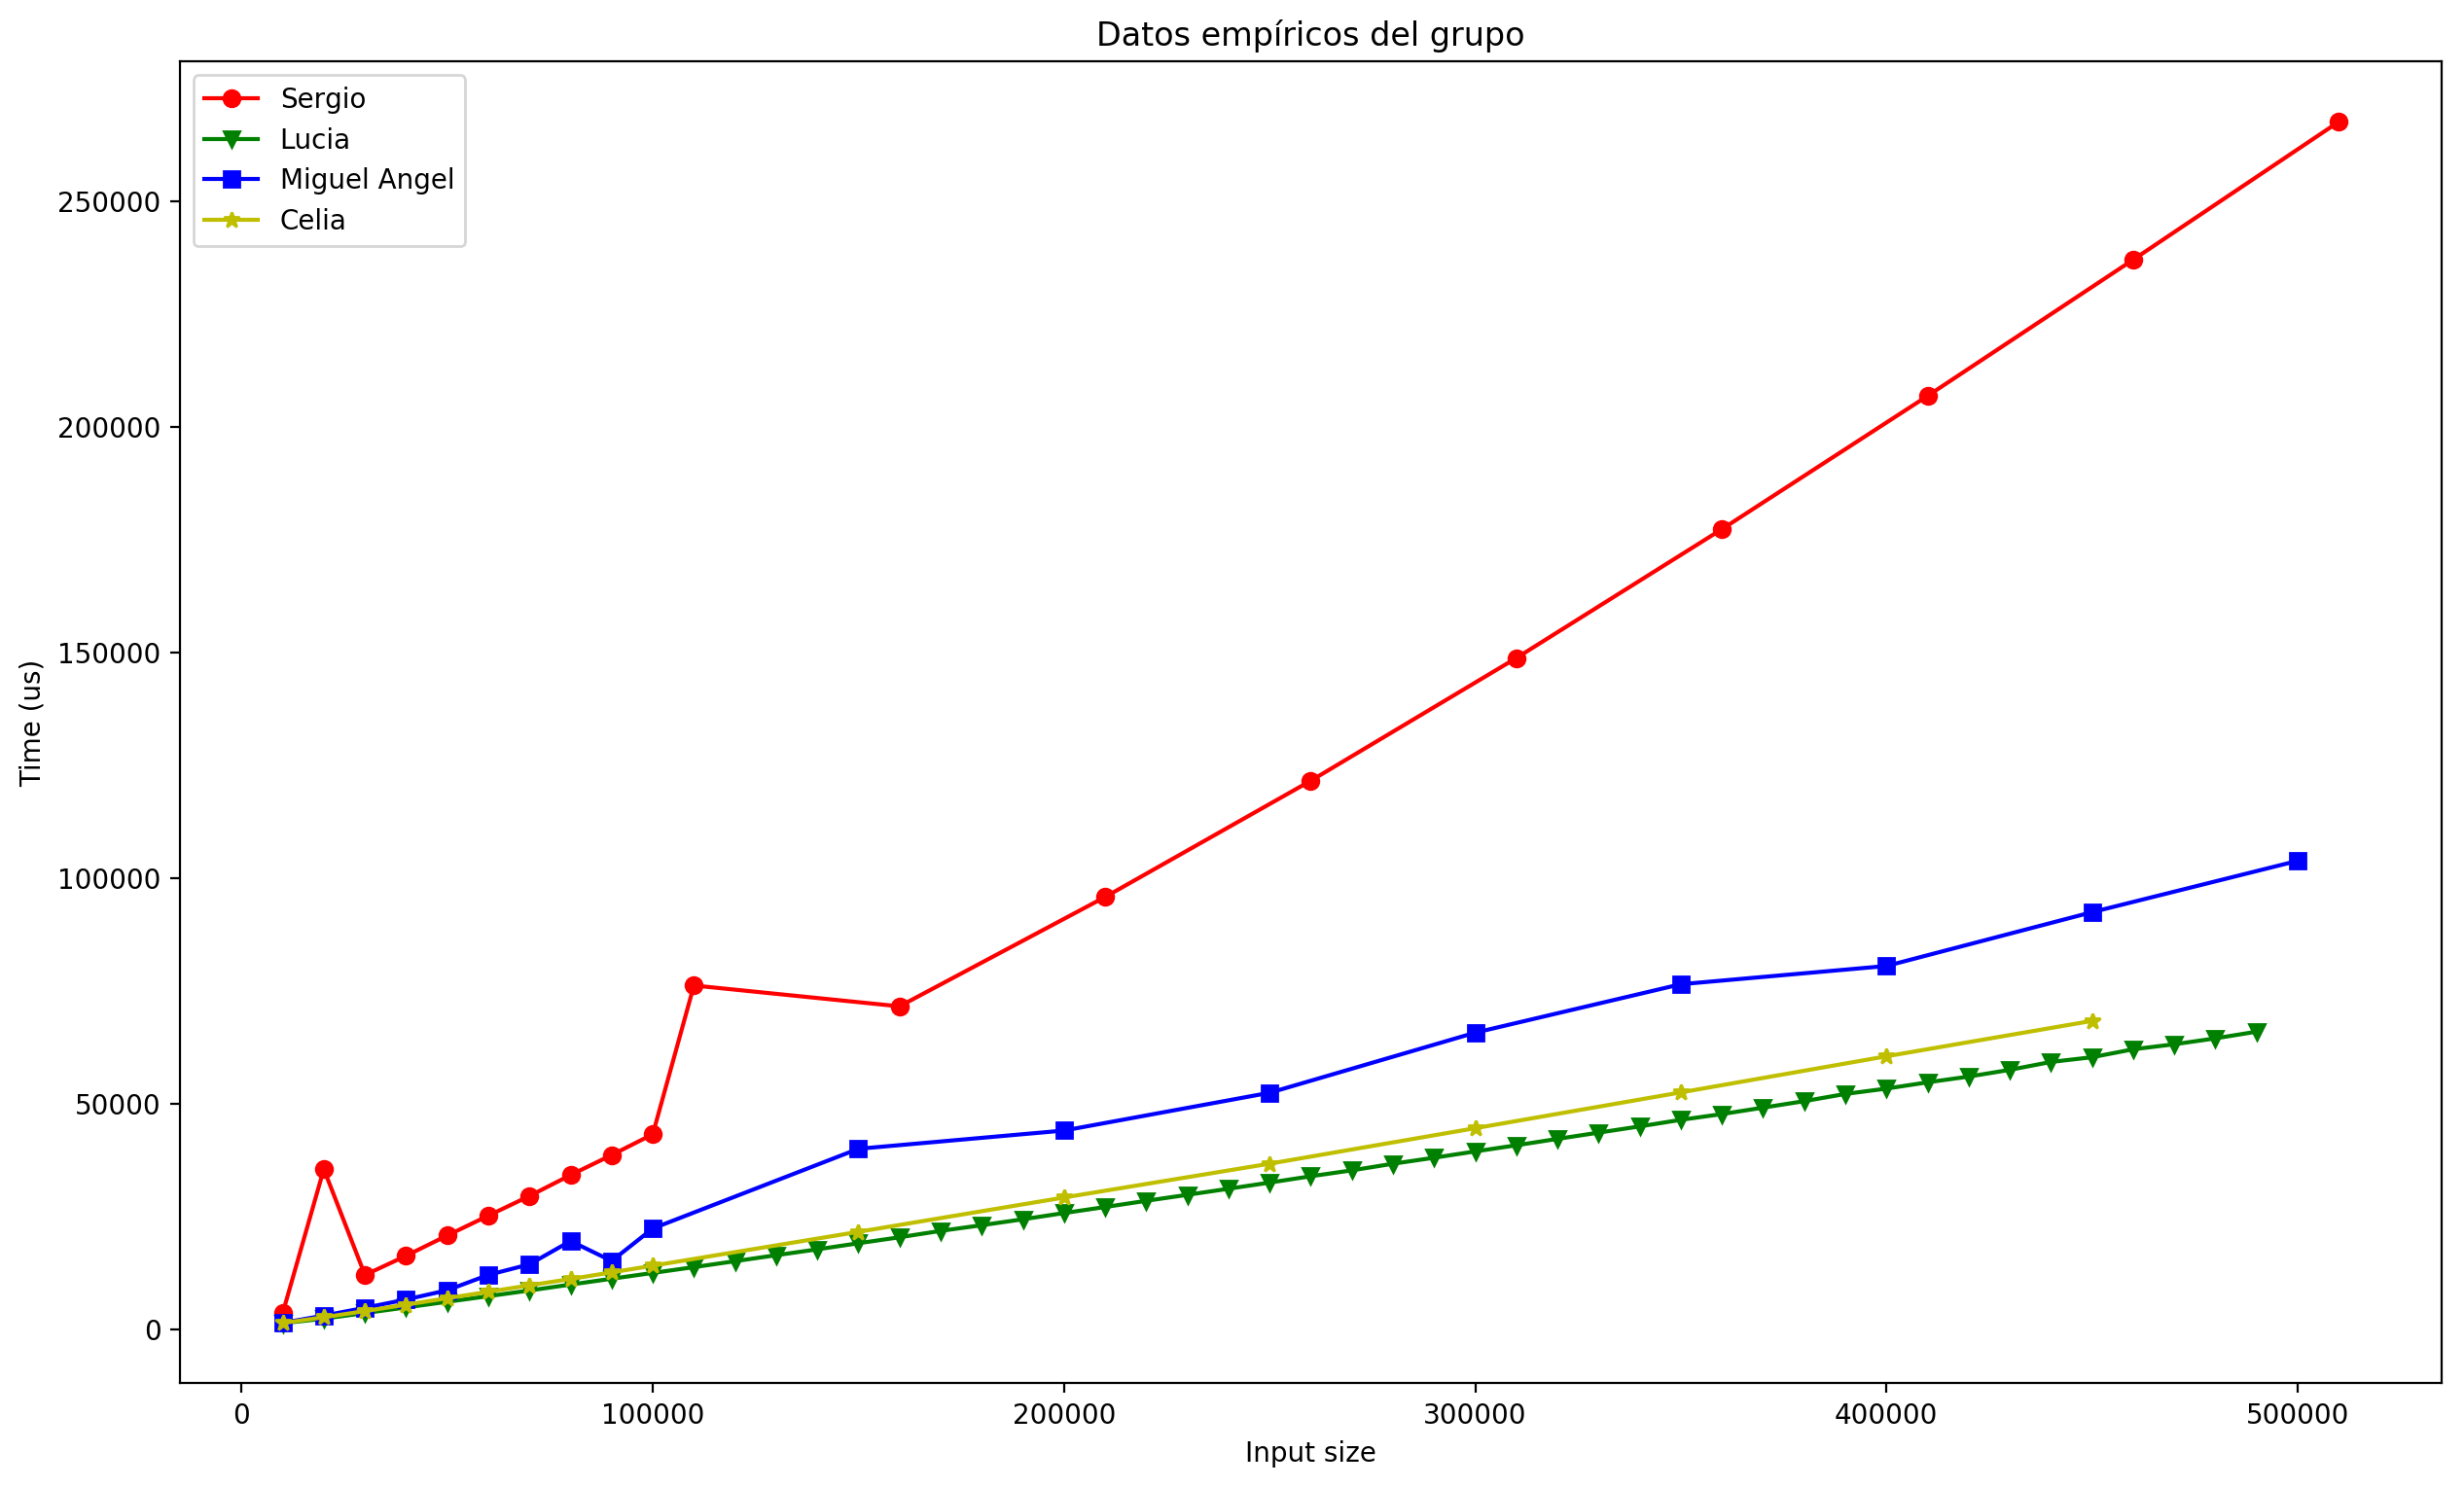
\includegraphics[width=15cm]{./Graficas/heap_todos.png}}

\newcommand{\autor}{Celia Ars Martínez\\Miguel Ángel Fernández Gutiérrez\\Sergio Quijano Rey\\Lucía Salamanca López}

\newcommand{\grado}{segfault}

\newcommand{\universidad}{Universidad de Granada}

\newcommand{\enlaceweb}{github.com/DGIIMUnderground}

% ---------------------------------------------------------------------------
% CONFIGURACIÓN PERSONALIZADA
% ---------------------------------------------------------------------------

%%%%%%%%%%%%%%%%%%%%%%%%%%%%%%%%%%%%%%%%%%%%%%%%%%%%%%%%%%%%%%%%%%%%%%%%%%%%%
% ---------------------------------------------------------------------------
% COMIENZO DEL DOCUMENTO
% ---------------------------------------------------------------------------
%%%%%%%%%%%%%%%%%%%%%%%%%%%%%%%%%%%%%%%%%%%%%%%%%%%%%%%%%%%%%%%%%%%%%%%%%%%%%

\begin{document}

% ---------------------------------------------------------------------------
% PORTADA EXTERIOR
% ---------------------------------------------------------------------------

\newpagecolor{500}\afterpage{\restorepagecolor} % Color de la página
\begin{titlepage}

  % Título del documento
	\parbox[t]{\textwidth}{
			\raggedright % Texto alineado a la izquierda
			\fontsize{40pt}{40pt}\selectfont\sffamily\color{white}{
				\textbf{\Huge{Práctica 1}}\\\textbf{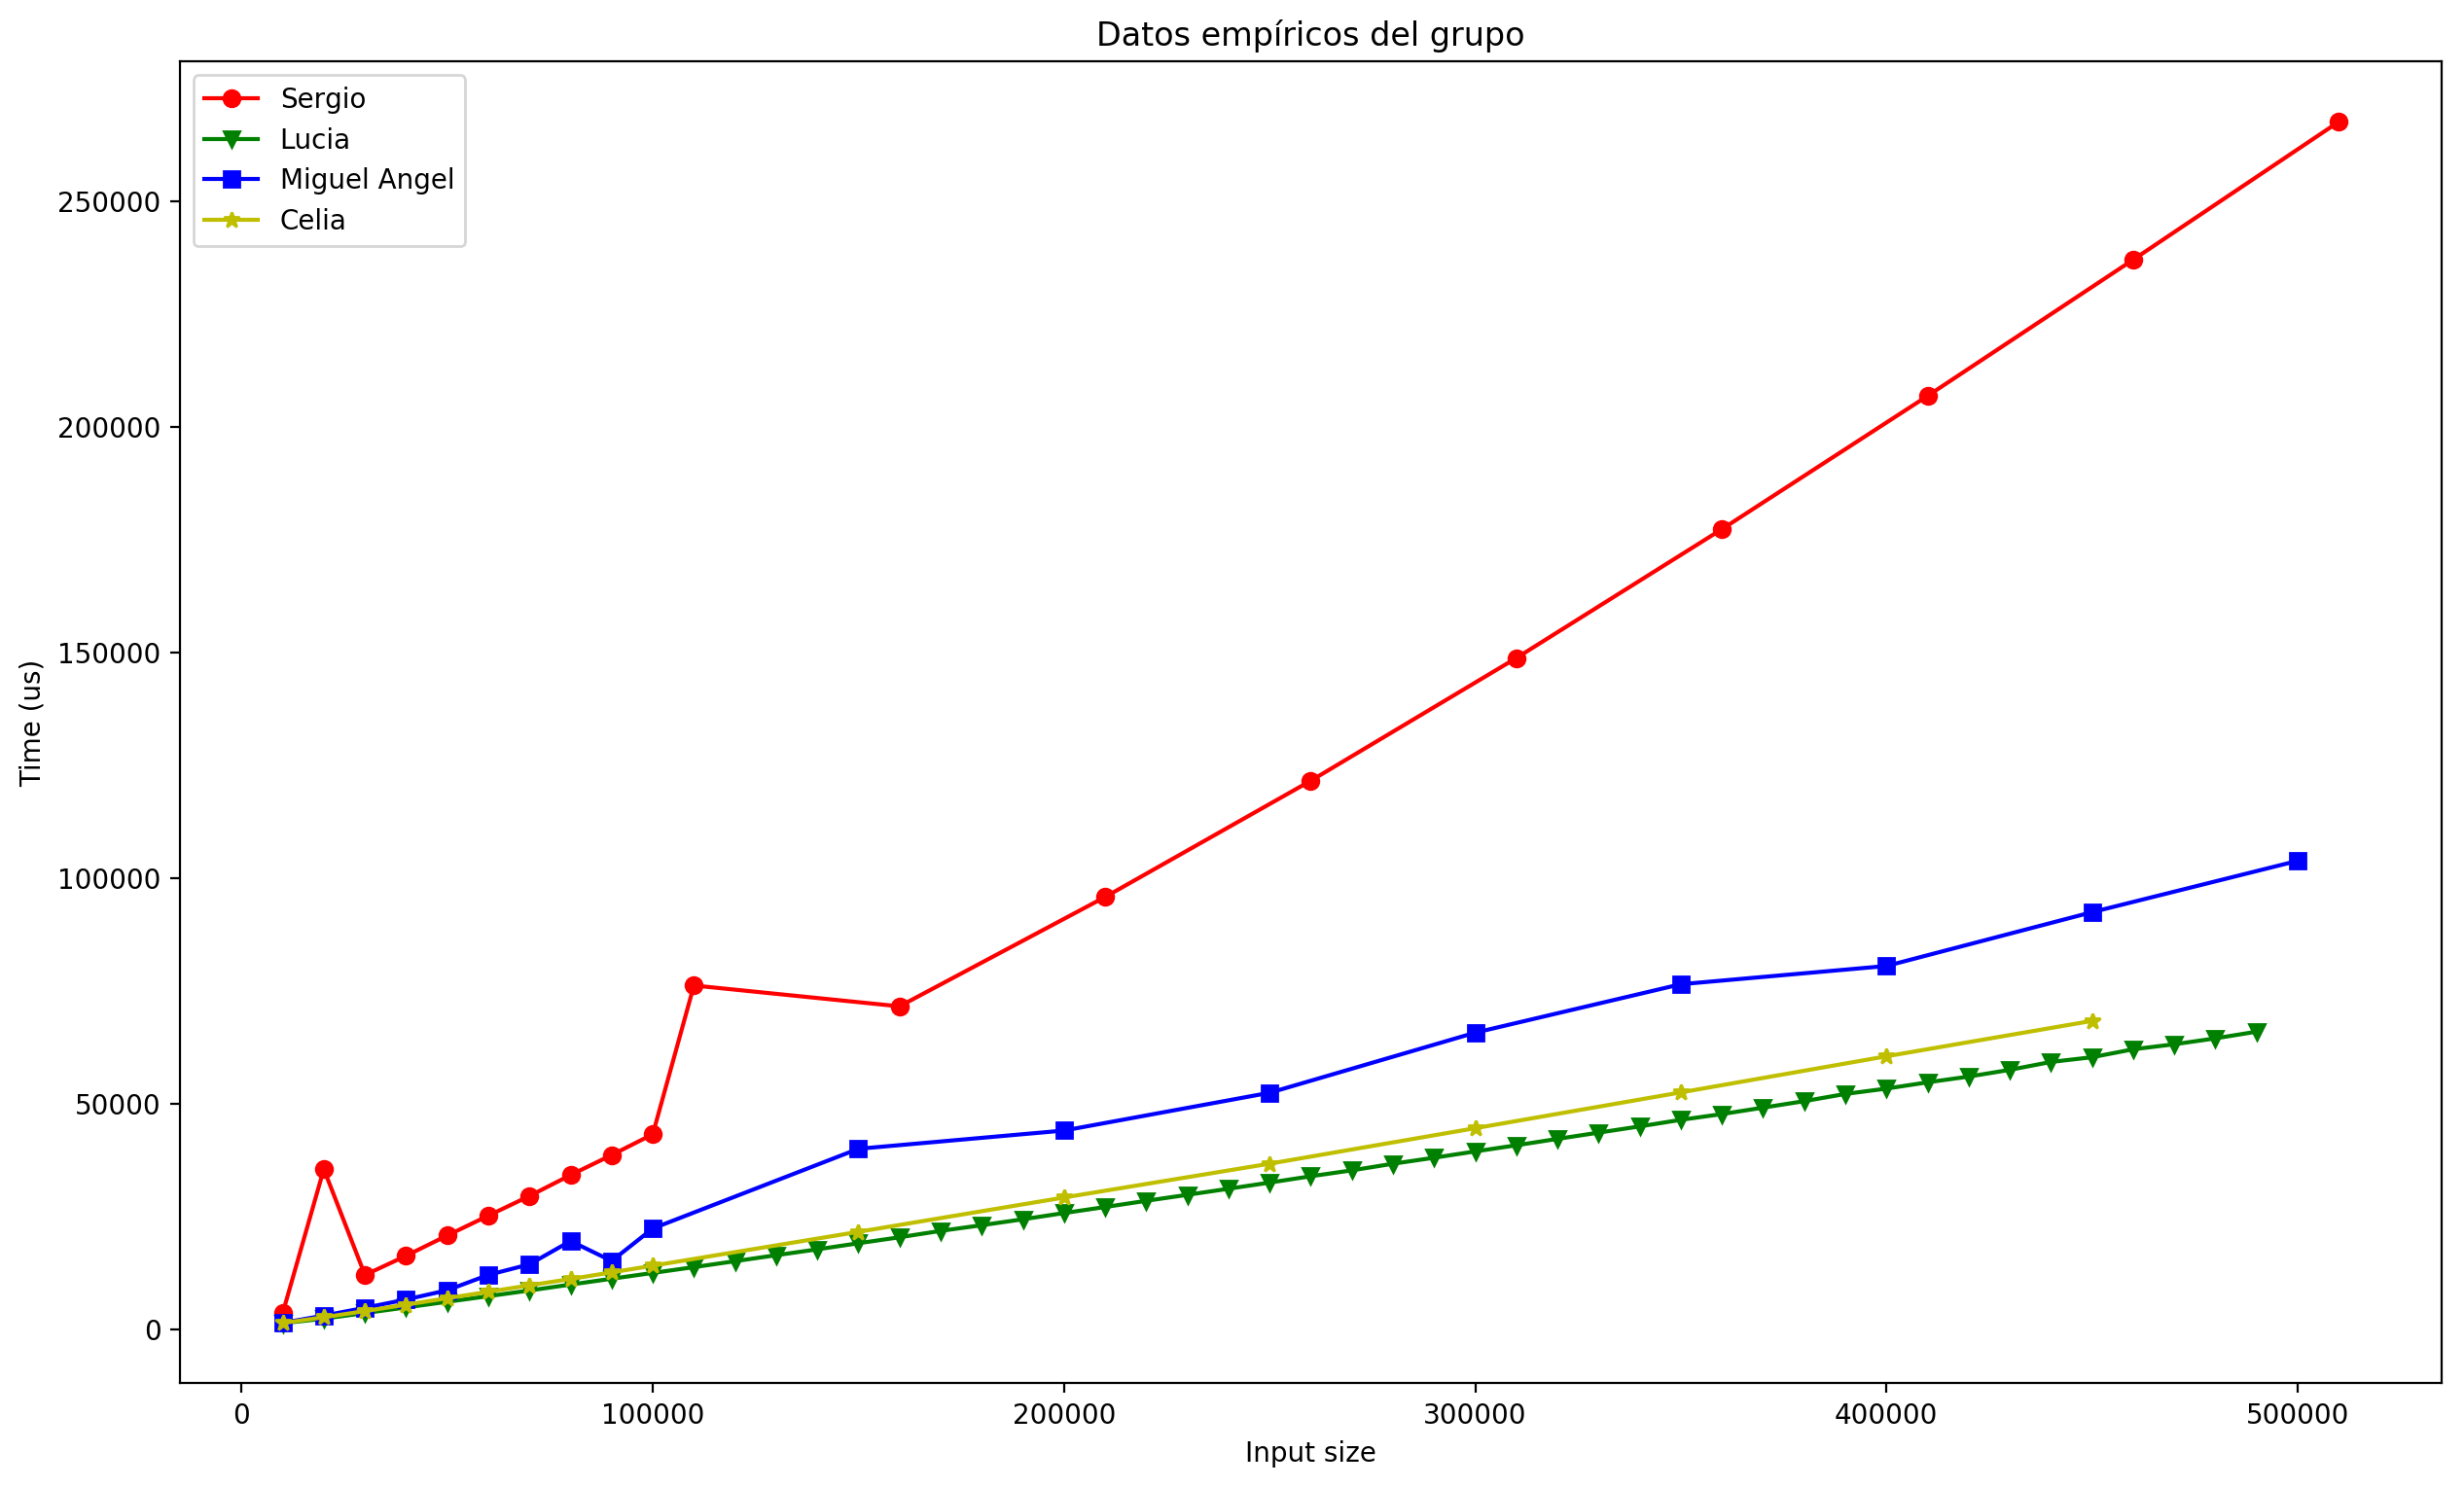
\includegraphics[width=15cm]{./Graficas/heap_todos.png}}\\\huge{Algorítmica}
      }
	}

	\vfill

	%% Autor e información del documento
	\parbox[t]{\textwidth}{
		\raggedright % Texto alineado a la izquierda
		\sffamily\large\color{white}
		\grado\\
		{\Large \autor }\\[15pt]
		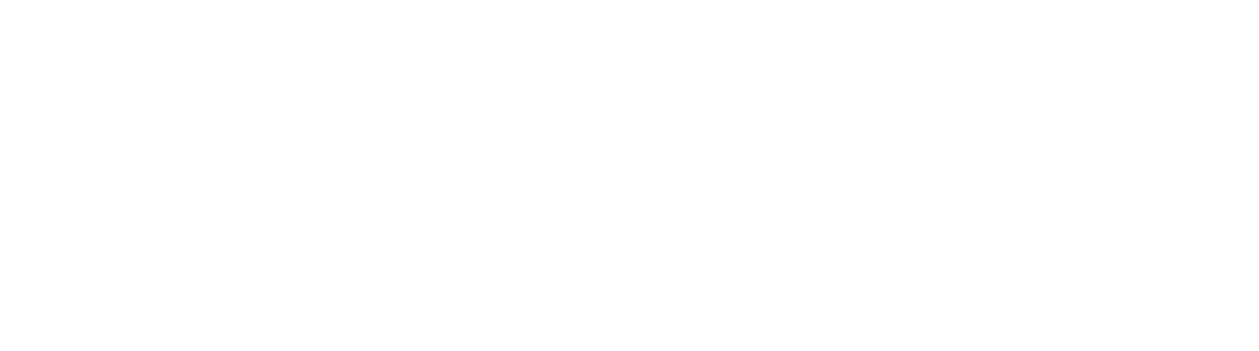
\includegraphics[width=130pt]{ugrlogo.pdf}
	}

\end{titlepage}

% ---------------------------------------------------------------------------
% PÁGINA DE LICENCIA
% ---------------------------------------------------------------------------

\thispagestyle{empty}
\null
\vfill

%% Información sobre la licencia
\parbox[t]{\textwidth}{
  
\includegraphics{by-nc-sa.pdf}\\[4pt]
  \raggedright % Texto alineado a la izquierda
  \sffamily\large
  {\Large Este trabajo se distribuye bajo una licencia CC BY-NC-SA 4.0.}\\[4pt]
  Eres libre de distribuir y adaptar el material siempre que reconozcas a los\\
  autores originales del documento, no lo utilices para fines comerciales\\
  y lo distribuyas bajo la misma licencia.\\[4pt]
  \texttt{creativecommons.org/licenses/by-nc-sa/4.0/}
}

% ---------------------------------------------------------------------------
% PORTADA INTERIOR
% ---------------------------------------------------------------------------

\begin{titlepage}

  % Título del documento
  \parbox[t]{\textwidth}{
  	\raggedright % Texto alineado a la izquierda
  	\fontsize{40pt}{40pt}\selectfont\sffamily\color{500}{
  		\textbf{\Huge{Práctica 1}}\\\textbf{Análisis de eficiencia\\de algoritmos}\\\huge{Algorítmica}
  	}
  }

	\vfill
	
	%% Autor e información del documento
	\parbox[t]{\textwidth}{
		\raggedright % Texto alineado a la izquierda
		\sffamily\large
		\grado\\
		{\Large \autor }\\[15pt]
		
\includegraphics[width=130pt]{ugrlogo-dark.pdf}
	}

\end{titlepage}

% ---------------------------------------------------------------------------
% ÍNDICE
% ---------------------------------------------------------------------------

\thispagestyle{empty}
\tableofcontents
\newpage

% ---------------------------------------------------------------------------
% CONTENIDO
% ---------------------------------------------------------------------------

\part{¿Qué es una criptomoneda?}

\textbf{Bitcoin} es una de las criptomonedas más conocidas. Sepamos bien
cómo funciona o no, todos hemos oído hablar de Bitcoin. Sin embargo, hay
muchas otras, que se basan en los mismos principios básicos. Por tanto,
para explicar las criptomonedas, veamos cuáles son estos principios.

Supongamos que queremos crear una criptomoneda, \emph{DGIIMCoin}. La
primera pregunta sería para qué, y la segunda --en caso de que el para
qué nos haya convencido-- es qué necesitamos para ello.

Crear todo esto tendría sentido si queremos crear un sistema anónimo,
descentralizado y seguro para intercambiar dinero o información. Veamos
bien qué quiere decir esto:

\begin{itemize}
\itemsep1pt\parskip0pt\parsep0pt
\item
  \textbf{Anónimo:} los usuarios deben ser identificables para el sistema, pero
  su identidad debe ser custodiada con recelo.
\item
  \textbf{Descentralizado:} los sistemas convencionales depositan la confianza de
  instituciones en terceros --i.e. Amazon en el envío de bienes, un banco, etc.--,
  en el caso de las criptomonedas su estado es mantenido gracias al consenso de
  los usuarios.
\item
  Seguro:
\end{itemize}

Bien, para todo esto nuestro sistema debería tener una serie de
requisitos:

\begin{enumerate}
\def\labelenumi{\arabic{enumi}.}
\itemsep1pt\parskip0pt\parsep0pt
\item[\emph{Req. 1.}]
  El sistema no requiere de una \textbf{autoridad central}: su estado es
  mantenido mediante un \textbf{consenso} distribuido.
\item[\emph{Req. 2.}]
  El sistema mantiene un \textbf{seguimiento} de todas las unidades de
  la criptomoneda y de sus propietarios.
\item[\emph{Req. 3.}]
  El sistema define si se pueden crear \textbf{nuevas unidades} de la
  criptomoneda. Si esto es así, el sistema debe definir las
  circunstancias de su origen y cómo determinar quién será el
  propietario de éstas.
\item[\emph{Req. 4.}]
  La propiedad de las monedas puede probarse de forma exclusivamente
  \textbf{criptográfica}.
\item[\emph{Req. 5.}]
  El sistema permite la realización de \textbf{transacciones} de forma
  controlada.
\end{enumerate}

Nuestro sistema, por tanto, girará en torno a las siguientes ideas clave:

\begin{enumerate}
\itemsep1pt\parskip0pt\parsep0pt
\item
  \textbf{Descentralización.}
\item
  \textbf{Firmas digitales.}
\item
  \textbf{La contabilidad (\emph{ledger}) es la propia moneda.}
\item
  \textbf{Mecanismo de consenso.}
\item
  \textbf{Blockchain.}
\end{enumerate}

Explicaremos cada una de ellas con más detalle.

\section{Descentralización: redes
P2P}\label{compartiendo-informaciuxf3n-de-forma-descentralizada-redes-p2p}

Para poder cumplir los dos primeros requisitos de nuestra lista,
eliminando así autoridades centralizadas, temos ya una solución
disponible: las \textbf{redes \emph{peer-to-peer}}, o \textbf{redes
P2P}.

La idea principal de estas redes es que la información se comparta de
igual a igual, al contrario a las redes cliente-servidor. En este caso,
todos los ordenadores tienen el mismo peso.

{[}Más de P2P{]}

En definitiva, podemos usar los protocolos P2P existentes para
implementar \emph{DGIIMCoin}. Genial, continuemos.

\section{Firmas digitales, criptografía y
\emph{hashing}}\label{firmas-digitales-criptografuxeda-y-hashing}

Para que nuestro sistema funcione son esenciales las \textbf{identidades
digitales}, es decir, formas de verificar que una transacción se ha
hecho realmente (alguien de verdad ha enviado dinero a otra persona).
Para eso, usamos la \textbf{criptografía}.

{[}Más de criptografía y hashing{]}

\section{Enviando transacciones a la
red}\label{enviando-transacciones-a-la-red}

Ya casi estamos. Hemos implementado comunicación P2P, mecanismos para
crear identidades digitales y formas para que los usuarios puedan firmar
y garantizar que la información es correcta. Ahora sólo nos queda enviar
información al sistema.

Como ya sabemos, no tenemos una autoridad central que valide cuánto
dinero tenemos, pero tampoco hace falta: aquí reside una de las ideas,
que la \textbf{contabilidad es la propia moneda}. Esto se debe a que
para saber cuánto dinero tenemos, simplemente nos basta con tener una
lista de todas las transacciones que hemos efectuado. Supongamos que tu
historial de transacciones contiene la información:

\begin{enumerate}
\def\labelenumi{\arabic{enumi}.}
\itemsep1pt\parskip0pt\parsep0pt
\item
  Tengo 500 \dout{D}.
\item
  Envío 20 \dout{D} a alguien para unos apuntes de Modelos de
  Computación (incluiremos su clave pública).
\item
  Quiero enviar 1 \dout{D} como impuesto de transacción al sistema (lo
  veremos más adelante).
\item
  Quiero quedarme con las \emph{DGIIMCoins} restantes.
\end{enumerate}

Lo único que queda es usar la red P2P para enviar estas transacciones al
resto de usuarios del sistema, sin olvidar de firmarlas usando nuestra
clave privada. Tras esto, todo el mundo sabrá que has pagado 20 \dout{D}
a tu compañero por apuntes.

Listo. Sin embargo, no tendrás los apuntes hasta que la red coincida en
que inicialmente tenías 500 \dout{D}, y por tanto dicha transacción
puede efectuarse. Una vez que la transacción se valide, tu compañero te
dará los apuntes.

\section{Mecanismos de verificación de
transacciones}\label{mecanismos-de-verificaciuxf3n-de-transacciones}

\subsection{Mining: proof-of-work}\label{mining-proof-of-work}

\subsection{Otros mecanismos}\label{otros-mecanismos}

\subsubsection{Proof-of-burn}\label{proof-of-burn}

\subsubsection{Proof-of-stake}\label{proof-of-stake}

\subsubsection{Proof-of-capacity}\label{proof-of-capacity}

\subsubsection{Proof-of-elapsed time}\label{proof-of-elapsed-time}

\subsubsection{Proof-of-importance}\label{proof-of-importance}

\section{El blockchain}\label{el-blockchain}

\section{Controlando la fuente de
dinero}\label{controlando-la-fuente-de-dinero}

\part{Aplicaciones de las
criptomonedas}\label{aplicaciones-de-las-criptomonedas}

\part{Nuevas criptomonedas}\label{nuevas-criptomonedas}

Criptomonedas de segunda y tercera generación. Conceptos.

\part{Demo: Wireshark}\label{demo-wireshark}



\part{Introducción}

Esta \textbf{práctica 1}, de análisis de eficiencia de algoritmos, consiste en tres partes:

\begin{itemize}
	\item \textbf{Análisis de la eficiencia teórica:} predicción de clase de eficiencia.
	\item \textbf{Análisis de la eficiencia empírica:} ejecución y medición de tiempos.
	\item \textbf{Análisis de la eficiencia híbrida:} obtención de la constante oculta.
\end{itemize}

A continuación, se explican en más profundidad dichas partes.

\subsection*{Análisis de la eficiencia teórica}

El análisis de la eficiencia \textbf{teórica} consiste en analizar el tiempo de ejecución en peor caso de los algoritmos, para decidir en qué clase de funciones en notación $O$ grande se encuentra. Para ello, hemos utilizado las técnicas de análisis y de resolución de recurrencias que han sido explicadas en clase.

\subsection*{Análisis de la eficiencia empírica}

Para el análisis de la eficiencia empírica, hemos ejecutado todos los algoritmos en cada uno de nuestros ordenadores, y los hemos medido con la biblioteca \texttt{<chrono>}, haciendo uso del siguiente esquema de código:

\begin{lstlisting}[language=C]
chrono::time_point<std::chrono::high_resolution_clock> t_ini, t_fin;

...

t_ini = chrono::high_resolution_clock::now();

// se ejecuta el algoritmo cuyo tiempo se quiere medir
ejecutarAlgoritmo();

t_fin = chrono::high_resolution_clock::now();
\end{lstlisting}

Hemos ejecutado cada algoritmo 100 veces en cada uno de los tamaños que han sido probados (y los cuales se especifican en el apartado de \emph{eficienicia empírica} de cada uno de éstos), y hemos hecho la media de ellos para reducir las perturbaciones que puedan ocurrir azarosamente y que nos lleven al mejor o peor caso, obteniendo de esta forma casos promedio.

Nótese que, en los algoritmos de búsqueda, hemos elegido los mismos intervalos de datos para poder comparar los tiempos y ver la diferencia entre un orden de eficiencia y otro. Esta comparación se realizará en el apartado \emph{Conclusiones}).

Evidentemente, los resultados han variado de acuerdo a cada uno de nuestros ordenadores.

\subsection*{Análisis de la eficiencia híbrida}

Para el análisis de la eficiencia híbrida, hemos tomado los datos de uno de los alumnos del grupo y hemos hallado la $K$ (constante oculta). Para ello, hemos procedido de dos maneras:

\begin{itemize}
	\item Tal y como está especificado en el guion de prácticas: hemos realizado la división $\frac{T(n)}{f(n)}$ para cada una de las muestras medias.
	\item Por otro lado, hemos calculado la constante oculta $K$ mediante la búsqueda de la mejor función de la clase de equivalencia de las funciones $O(T(n))$, y tomando su coeficiente, con la ayuda de \emph{Jupyter}.
\end{itemize}

\pagebreak
\part{Desarrollo}

A continuación, realizaremos el estudio individual de cada algoritmo, como se ha descrito anteriormente.

\section{Algoritmo de pivote}

\begin{lstlisting}[language=C]
int pivotar(double *v, const int ini, const int fin) {
	double pivote = v[ini];
	double aux;
	
	int i = ini + 1;
	int j = fin;
	
	while ( i <= j ) {
		while ( v[i] < pivote && i <= j ) {
			i++;
		}
	
		while ( v[j] == pivote && j >= i ) {
			j--;
		}
		
		if ( i < j ) {
			aux = v[i];
			v[i] = v[j];
			v[j] = aux;
		}
		
		if ( j < ini ) {
			v[ini] = v[j];
			v[j] = pivote;
		}
		
		return j;
	}
}
\end{lstlisting}

\subsection{Eficiencia teórica}

Las operaciones en las \emph{líneas 5-9} son $O(1)$. Nos interesa estudiar el bucle externo y los dos bucles internos. Los \texttt{if} internos son $O(1)$, por tanto, de éstos solo nos interesa como afectan a los tres bucles que estudiamos. Estos \texttt{if} determinan si hay un cambio en el vector o no; esto no nos interesa, no afectan a los contadores y son $O(1)$.

El bucle \texttt{while} externo se ejecuta, si notamos $n=\texttt{j}-\texttt{i}$, $n$ veces. Nos interesa por tanto el número de veces que ejecutamos el bucle y el tiempo de ejecución del cuerpo del bucle.

Los dos bucles \texttt{while} internos hacen que se incremente el contador \texttt{i} y se decremente el contador \texttt{j}. En el peor caso, la variación de contadores será de uno en uno, para que la convergencia a la condición de salida ($\texttt{i} > \texttt{j}$) sea lo más lenta posible. Así, los dos bucles \texttt{while} internos son $O(1)$.

Con todo lo dicho, el cuerpo del \texttt{while} tiene una eficiencia $O(1)$, y al ejecutar el bucle $n$ veces, tenemos que:
$$ T(n) \in O(n) $$
Por tanto, nuestro algoritmo es $\boldsymbol{O(n)}$.

\section{Algoritmo de búsqueda binaria (versión iterativa)}

\begin{lstlisting}[language=C]
int Busqueda(int *v, int n, int elem){
	int inicio, fin, centro;

	inicio = 0;
	fin = n - 1;
	centro = ( inicio + fin ) / 2;

	while ( ( inicio <= fin ) && ( v[centro] != elem ) ) {
		if ( elem < v[centro] ) {
			fin = centro - 1;
		} else {
			inicio = centro + 1;
			centro = (inicio + fin) / 2;
		}
	}

	if ( inicio > fin ) {
		return -1;
	}
	
	return centro;
}
\end{lstlisting}

\subsection{Eficiencia teórica}

Nos encontramos ante un algoritmo de búsqueda binaria en su versión iterativa. La versión recursiva también se estudia más adelante en este documento. Para aplicar este algoritmo, lo lógico es que el vector sobre el que operamos esté ordenado, si no no tiene mucho sentido hacer la búsqueda binaria. A pesar de esto, a la hora de hacer el estudio de eficiencia teórica nos es igual. Lo único que pasaría es que el algoritmo casi nunca encontraría los valores, pero al estudiar el peor caso, el resultado será el mismo esté o no esté ordenado el vector sobre el que trabajamos.

Tanto las \emph{líneas 2-6} como las \emph{líneas 17-22} tienen una complejidad $O(1)$, por lo tanto nos interesa únicamente lo que ocurre en el cuerpo del \texttt{while}.

Al estar empleando la notación $O$ grande, nos situamos en el peor de los casos, como ya hemos razonado anteriormente. Por tanto, podemos suponer que no se va a encontrar el elemento buscado. Además, las \emph{líneas 9-14} son $O(1)$, de este modo, con lo anterior, solamente nos interesa la cantidad de veces que se ejecute el bucle \texttt{while}, sin tener en cuenta la segunda condición (como ya se ha dicho, suponemos que no se encuentra el elemento buscado).

Podemos suponer sin pérdida de generalidad que movemos el inicio hacia posiciones más avanzadas. En otro caso, podríamos pensar que trabajamos sobre el subvector de la izquierda en vez del subvector de la derecha, esto es indiferente a la hora de calcular el peor caso. 
$$ \texttt{inicio} = \frac{\texttt{inicio} + \texttt{fin}}{2} $$
Podemos tomar como tamaño de nuestro problema $size = \texttt{fin} - \texttt{inicio}$ para realizar el estudio. Con esto nos queda que el bucle \texttt{while} se ejecuta mientras $size \geq 1$ y que, en cada iteración, $size = \frac{size}{2}$.

Por tanto, falta resolver un $n_0$ mínimo tal que dividiendo $n_0$ veces $size$ se tenga 
$$ size \leq 1 $$
Podemos notar $size_i$ como el tamaño con el que trabajamos en la iteración $i$-ésima. Se verifica por tanto:
$$ size_i = \frac{size}{2^i} $$
Aplicando esto último a la condición $size \leq 1$ tenemos:
\begin{align*}
size_{n_0} &\leq 1\\
size_{n_0} = \frac{size}{2^n} &\leq 1
\end{align*}
Esto nos da claramente
$$ n_0 \geq \log_2{size} $$
Teniendo en cuenta que $size$ actúa como nuestro tamaño de caso, podemos reescribir la notación como $size \equiv n$, con lo que nos queda directamente:
$$ T(n) \in O(\log_2{n}) $$
Es decir, que nuestro algoritmo es $\boldsymbol{O(\log n)}$.

\section{Algoritmo de eliminación de repetidos}

\begin{lstlisting}[language=C]
void EliminaRepetidos(double original[], int & nOriginal){
	int i, j, k;
	
	for ( i = 0; i < nOriginal; i++ ) {
		j = i + 1;
		do {
			if ( original[j] == original[i] ){
				for ( k = j+1; k < nOriginal; k++ ) {
					original[k-1] = original[k];
					nOriginal--;
				}
			} else {
				j++;
			}
		} while ( j < nOriginal );
	}
}
\end{lstlisting}

\subsection{Eficiencia teórica}

Podemos estudiar distintas situaciones y ver cuál de ellas tiene una eficiencia peor, quedándonos con esta última. Los casos que podemos estudiar son los dos extremos (todo elemento está repetido una única vez, y no hay elementos repetidos) y el caso medio, algunos elementos repetidos.

\subsubsection*{Caso 1: Ningún elemento repetido}

Como en el resto de casos, el bucle \texttt{for} que empieza en la \emph{línea 4} se ejecuta $n$ veces. El cuerpo de este bucle equivale a tener un \texttt{for ( int j = i+2; j < nOriginal; j++ )}. Esto es debido a que nunca entramos en el \texttt{if} por no tener elementos repetidos. De este modo tenemos que:
$$ T_{\text{caso 1}} \in O(n^2)$$

\subsubsection*{Caso 2: Todos los elementos repetidos}

De nuevo, el bucle \texttt{for} externo se va a ejecutar $n$ veces, con la diferencia de que vamos a ir restando 1 a $n$ en cada iteración. Por tanto, en realidad ejecutamos este bucle $\frac{n}{2}$ veces.

En el \texttt{do-while} vamos a ejecutar el \texttt{for} una vez por iteración, y en cada \texttt{for} hacemos $n-h$ desplazamientos, para conveniente $h$. Por tanto, tenemos:
$$ T(n) \in O\left(\frac{n}{2} \cdot n\right) \equiv O(n^2) \longrightarrow T(n) \in O(n^2) $$

\subsubsection*{Caso 3: Algunos elementos repetidos}

Podríamos tratar de estudiar este caso, que es el más probable que se produzca, el caso promedio, pero sería bastante complicado. Como queremos saber cuál es el peor de los tres casos, podemos ver que este caso es más favorable que el \emph{Caso 2}, con lo que habríamos acabado.

Para ello solo hace falta pensar que podemos ver el vector como dos subvectores sobre los que aplicamos el algoritmo, un vector $v_1$ con ningún elemento repetido y un vector $v_2$ con todos los elementos repetidos al menos una vez. Podemos suponer, sin pérdida de generalidad, que $v_1$ se encuentra detrás de $v_2$, pues esto no afectará a la eficiencia. Sobre $v_1$ tenemos un $T_1(n) \in O(n^2)$. Sobre $v_2$ tenemos $T_{\text{caso 3}}(n) \leq T_{\text{caso 2}}(n)$. Esto es porque cabe la posibilidad de que un elemento esté más de una vez repetido, por lo que reduciríamos el tiempo de todos los desplazamientos posteriores.

Así tenemos que $T_{\text{caso 3}}(n) \leq T_{\text{caso 2}}(n)$, como se quería.

\subsubsection*{Conclusión}

Con todo lo dicho para los tres casos, hemos visto que
$$ T(n) \in O(n^2) $$
Por tanto, el algoritmo es $\boldsymbol{O(n^2)}$.

\section{Algoritmo de búsqueda binaria (versión recursiva)}

\begin{lstlisting}[language=C]
int BuscarBinario(int *v, const int ini, const int fin, const int x){
	int centro;
	
	if ( ini > fin )
		return -1;
	
	centro = ( ini + fin ) / 2;
	
	if ( v[centro] == x )
		return centro;
	
	if ( v[centro] > x )
		return BuscarBinario(v, ini, centro-1, x);
	
	return BuscarBinario(v, centro+1, fin, x);
}
\end{lstlisting}

\subsection{Eficiencia teórica}

Llamando $n$ al tamaño del vector, es decir, $n=\texttt{fin}-\texttt{ini}$. Las \emph{líneas 2-7}, así como las condiciones del \texttt{if} son $O(1)$. Como este algoritmo es recursivo, estudiaremos su comportamiento cada vez que vuelva a llamarse a sí mismo. En la $m$-ésima iteración y, suponiendo $-$en el peor caso$-$ que no encontramos el valor buscado, volvemos a llamar a la función con un subvector de tamaño $\frac{n}{2}$. De este modo, podemos establecer la siguiente relación de recurrencia:
$$T(m) = T\left(\frac{m}{2}\right)+1$$
Resolveremos esta recurrencia realizando la sustitución de $m$ por $2^k$, y despejando:
$$T(2^k)-T(2^{k-1})=1$$
Aplicamos las técnicas de resolución de recurrencias:
\begin{align*}
(x-1)^2 &= 0\\
t_{k} &= c_{1}*1^k + c_{2}*k*1^k\\
t_{k} &= c_{1}+c_{2}*k\\
t_{n} &= c_{1}+c_{2}*\log_{2}(n)
\end{align*}
En definitiva, obtenemos que nuestro algoritmo es $\boldsymbol{O(\log n)}$.

\subsection{Eficiencia empírica}

Tras ejecutar el algoritmo con variando el tamaño del vector \texttt{v} desde $10000$ hasta $100000$ en tramos de $10000$, y de ahí hasta $500000$ en tramos de $50000$; los resultados de ejecución para cada uno de los miembros del grupo fueron los siguientes:

\begin{datos}\hspace{-0.2cm}
	{\bf\sffamily Gráfico 4.1.} {\sffamily Datos de todas las ejecuciones}\\
	\vspace{-0.7cm}
	\begin{center}
		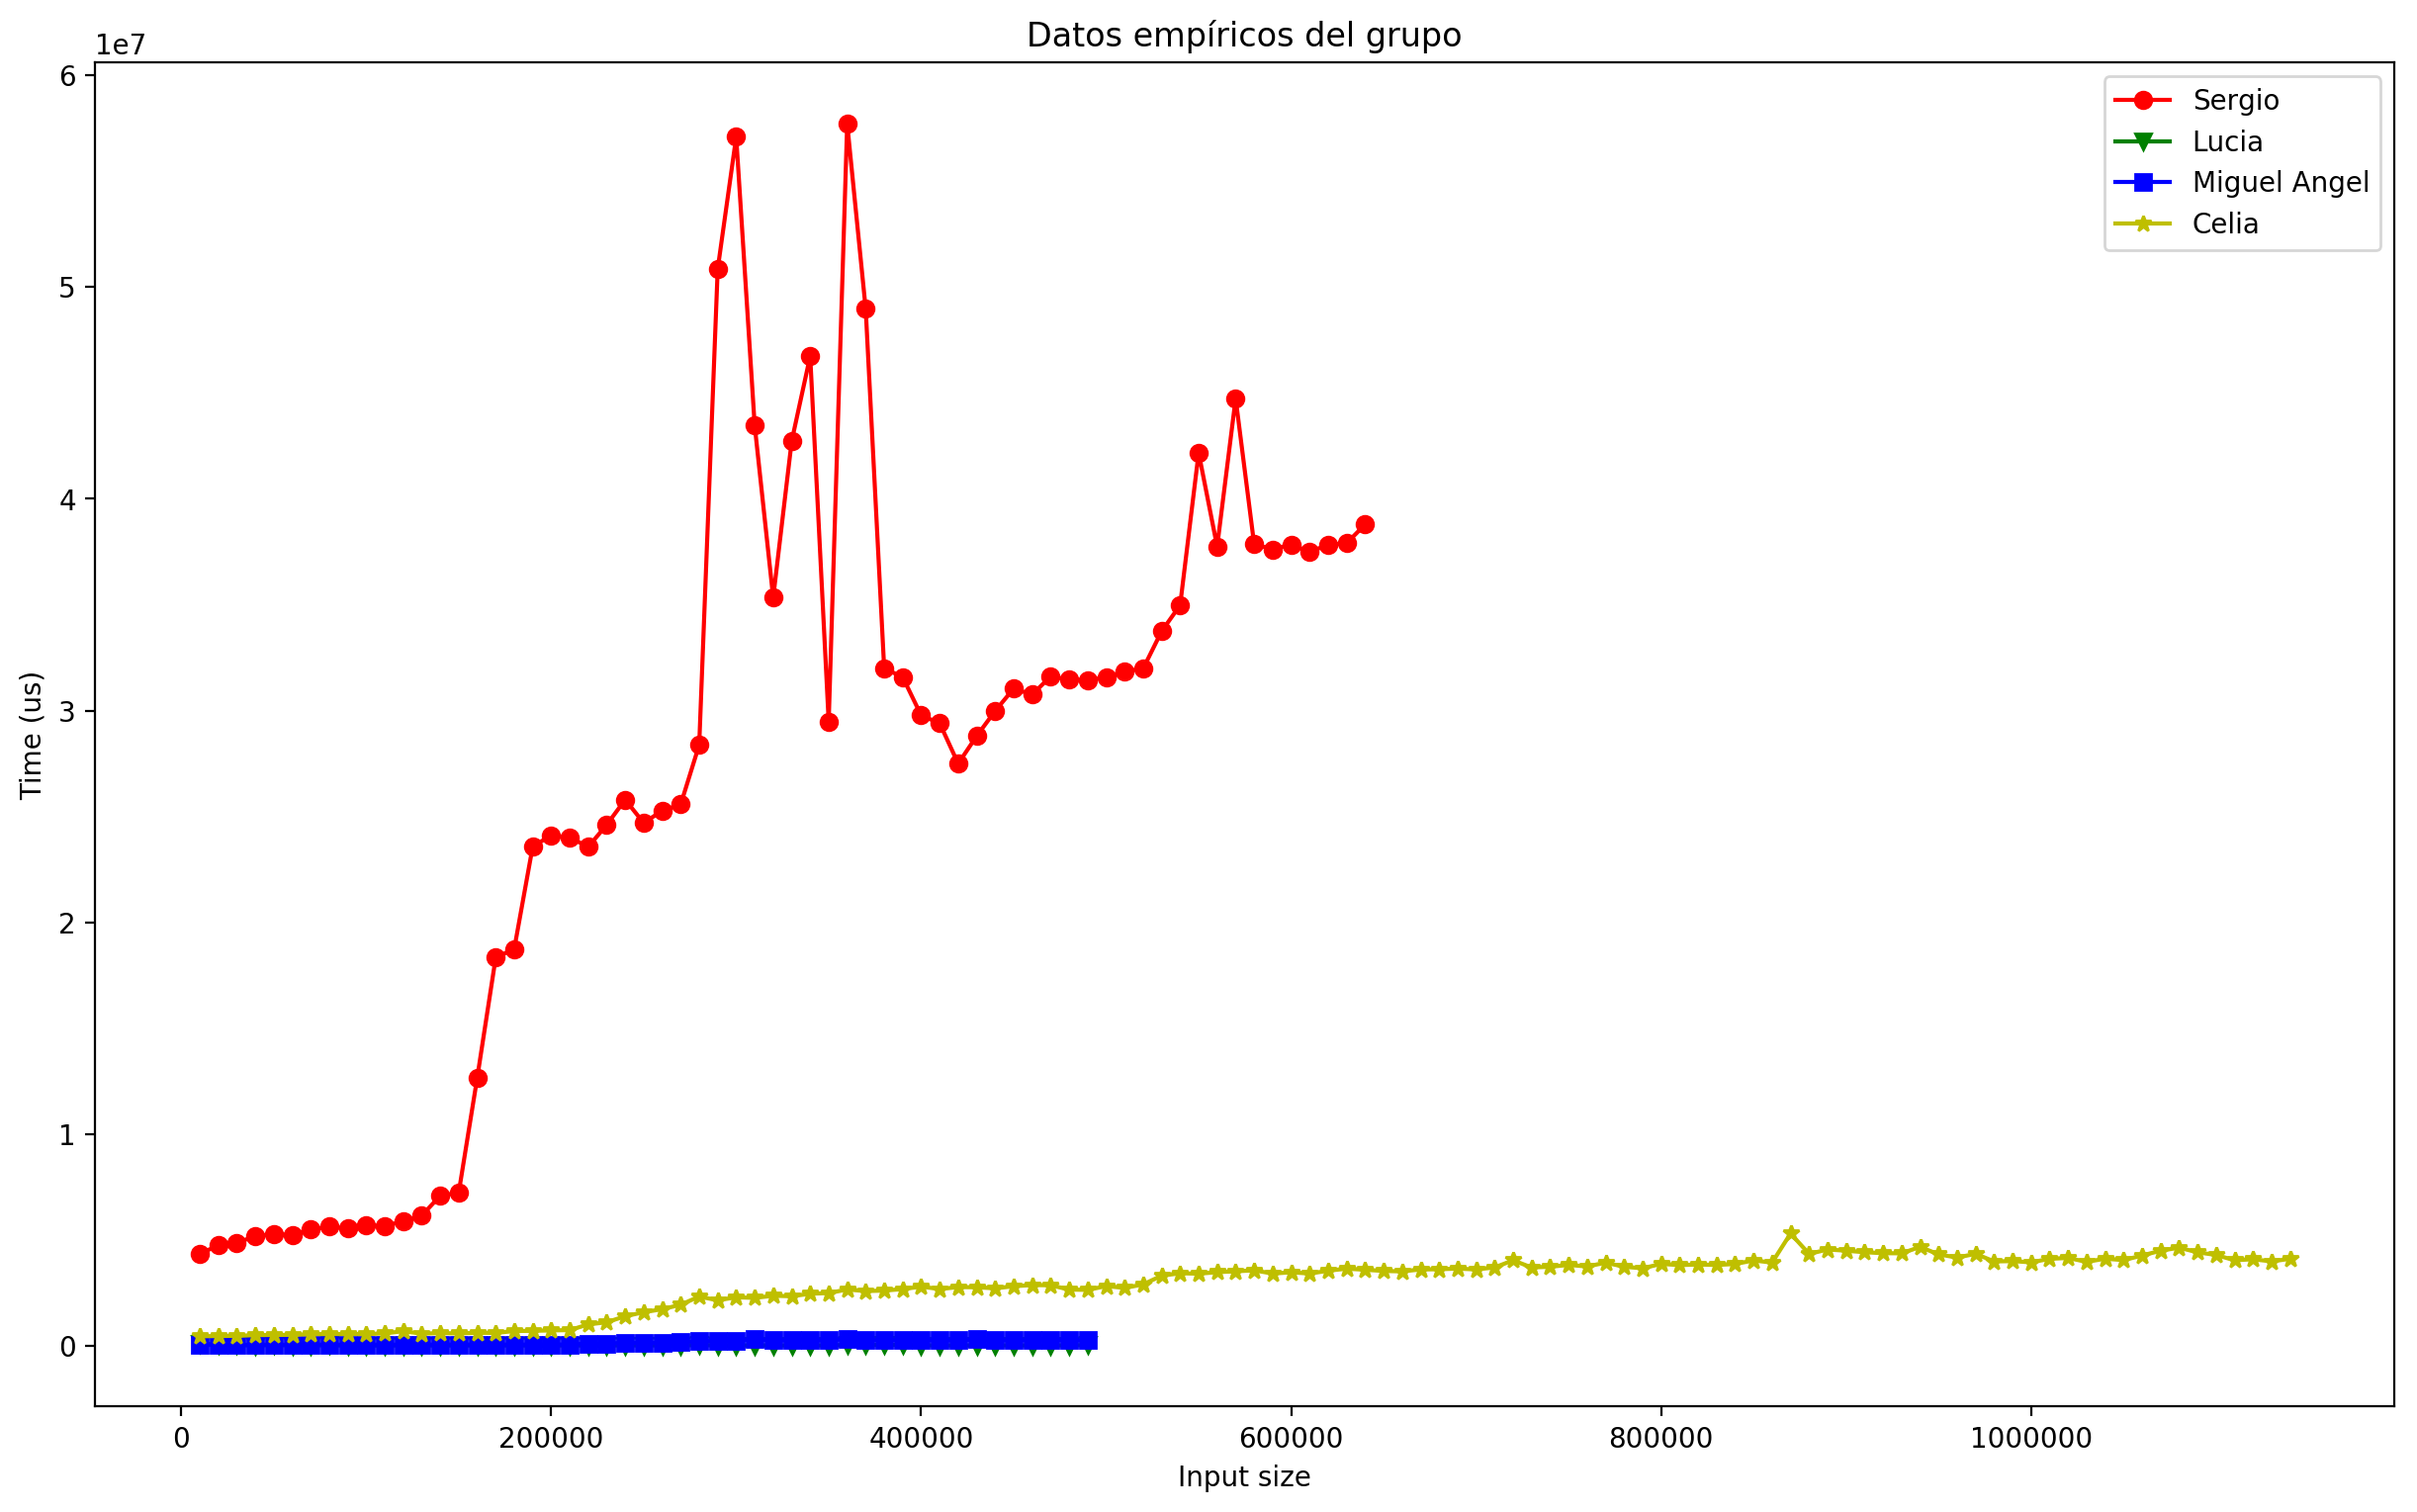
\includegraphics[width=15cm]{./Graficas/busquedabinaria_todos.png}
	\end{center}
\end{datos}

\subsection{Eficiencia híbrida}

A través de la eficiencia híbrida, comprobaremos que el ajuste teórico realizado es correcto.

Para realizar el análisis de la eficiencia híbrida, tomamos las ejecuciones de uno de los integrantes.
\pagebreak
\begin{datos}
	{\bf\sffamily Gráfico 4.2.} {\sffamily Datos que serán usados para el análisis híbrido}\\
	\vspace{-0.7cm}
	\begin{center}
		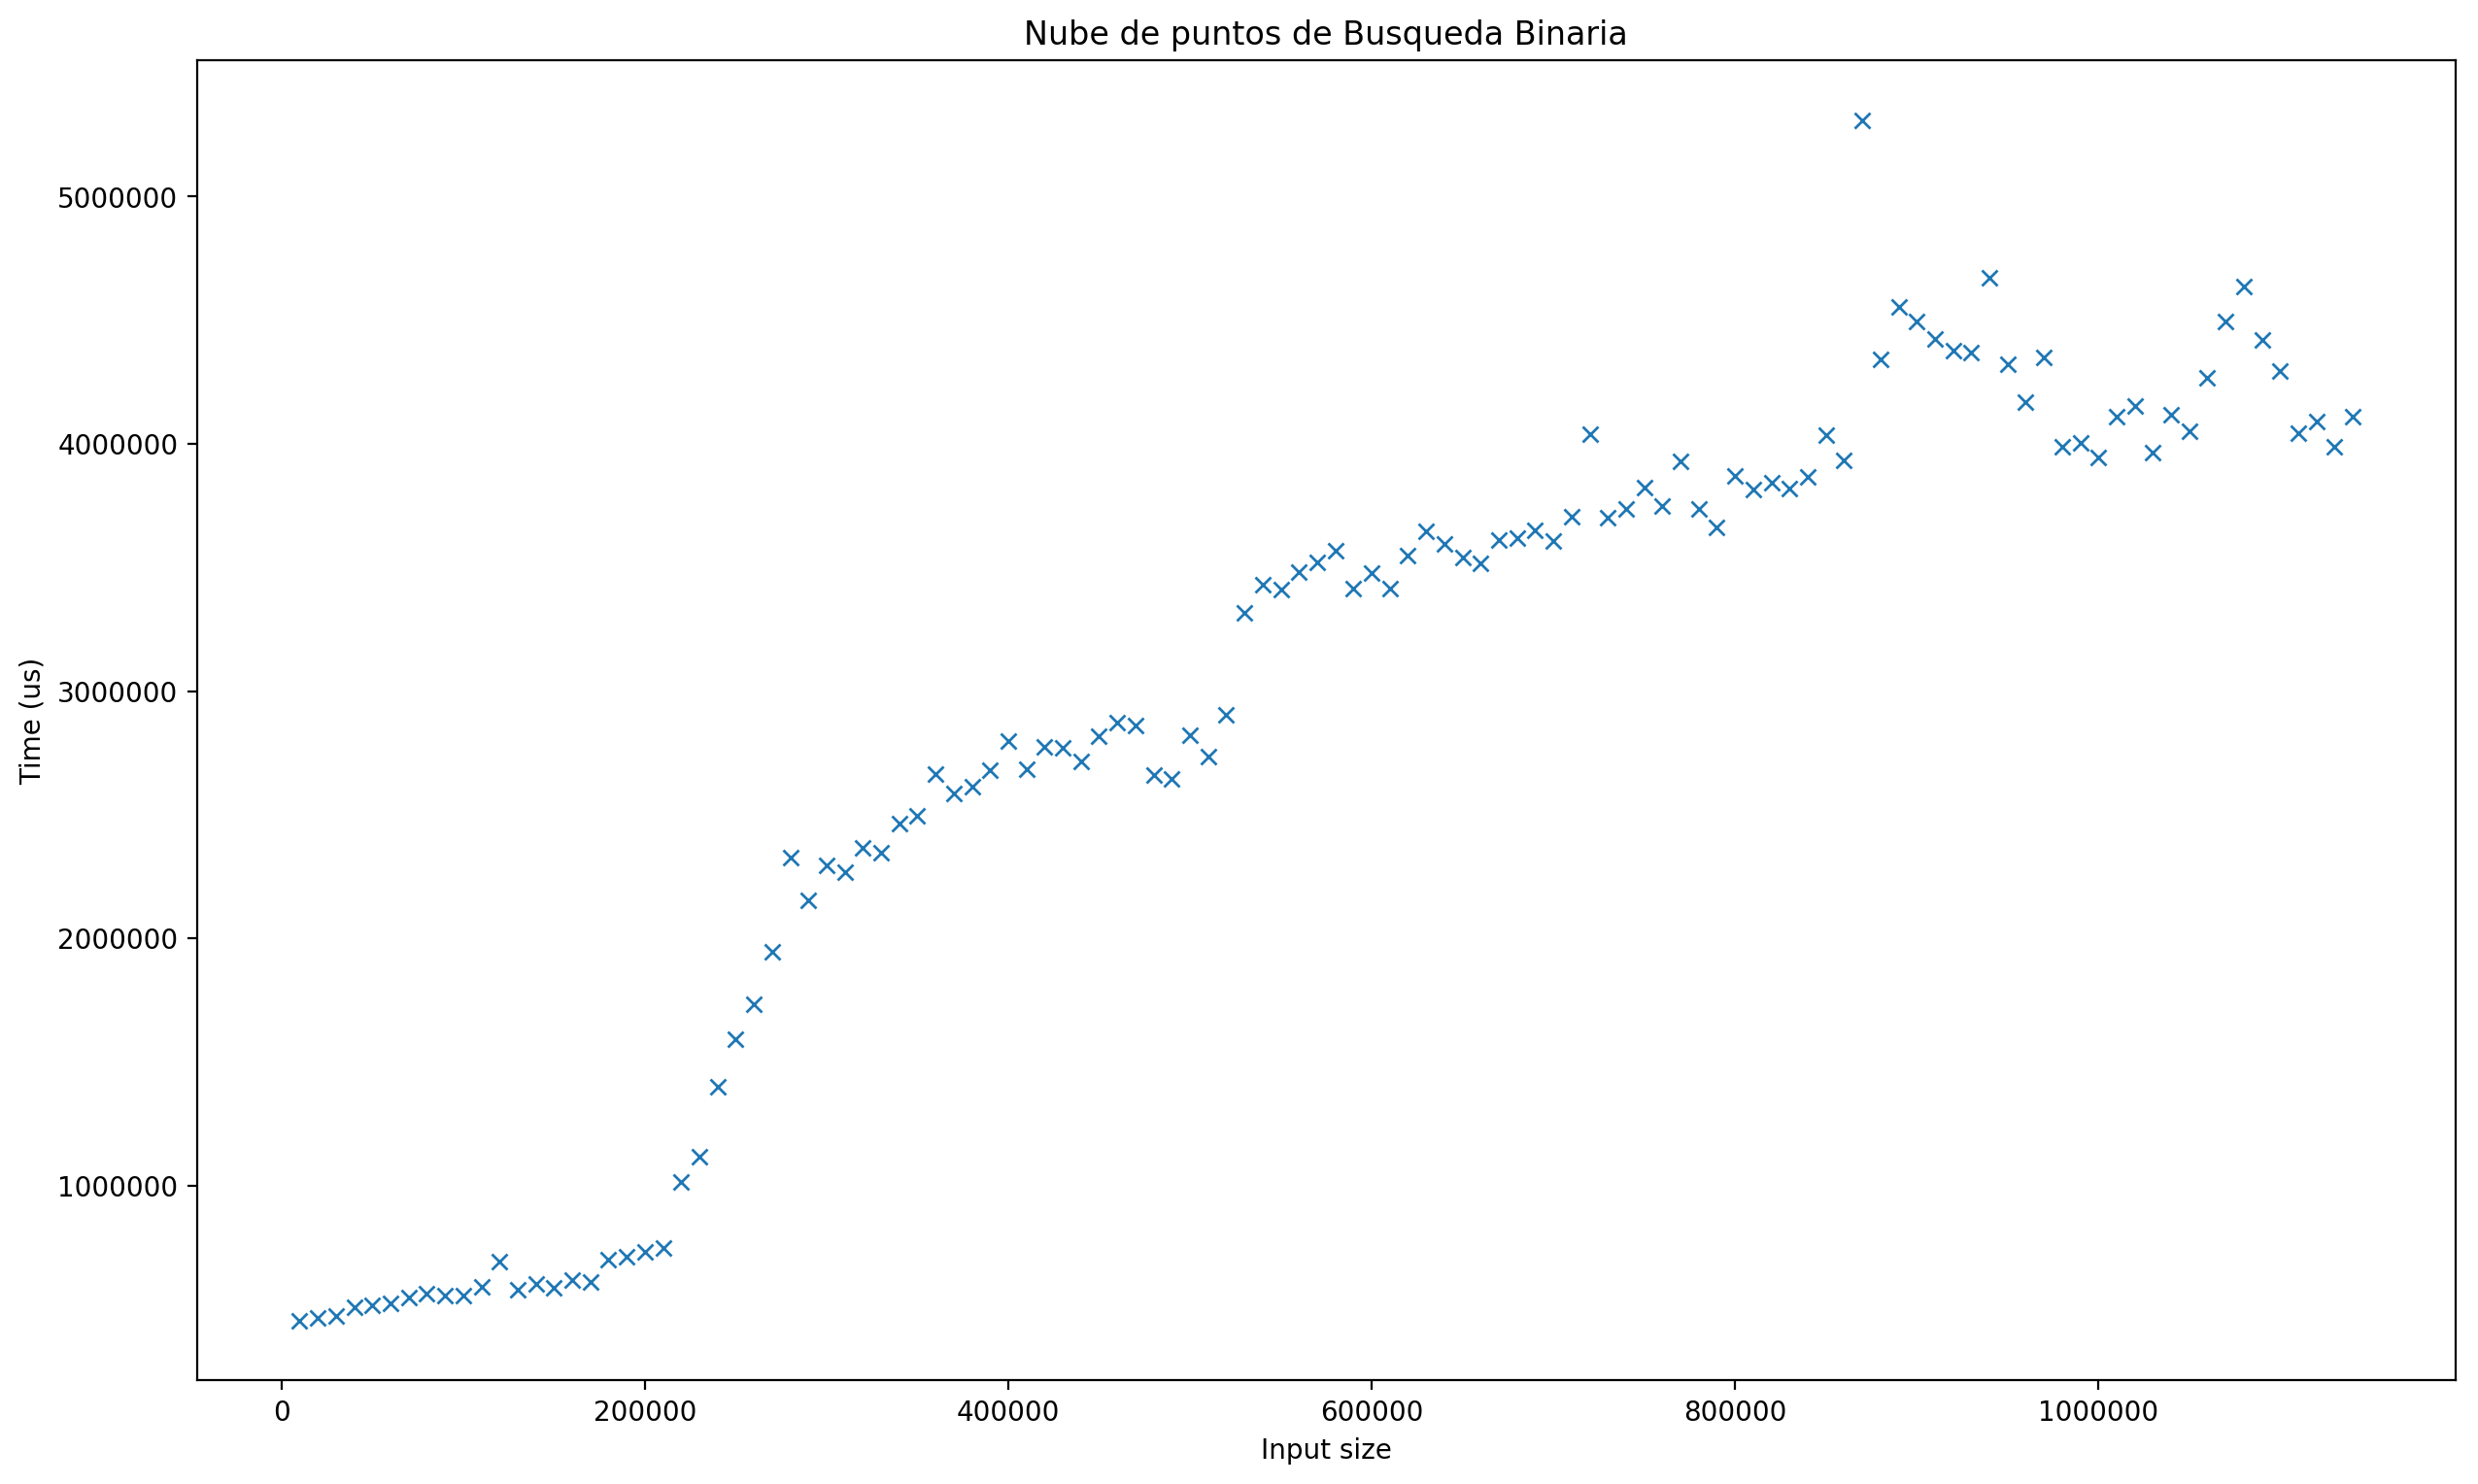
\includegraphics[width=15cm]{./Graficas/busquedabinaria_nube.png}
	\end{center}	
\end{datos}

\subsubsection{Ajuste de constante oculta}

Tras realizar el ajuste de la constante oculta, el valor obtenido es de $K=0.8630419355569797$.

\subsubsection{Ajuste por regresión}

\begin{datos}
	{\bf\sffamily Gráfico 4.3.} {\sffamily Ajuste por regresión}\\
	\vspace{-0.7cm}
	\begin{center}
		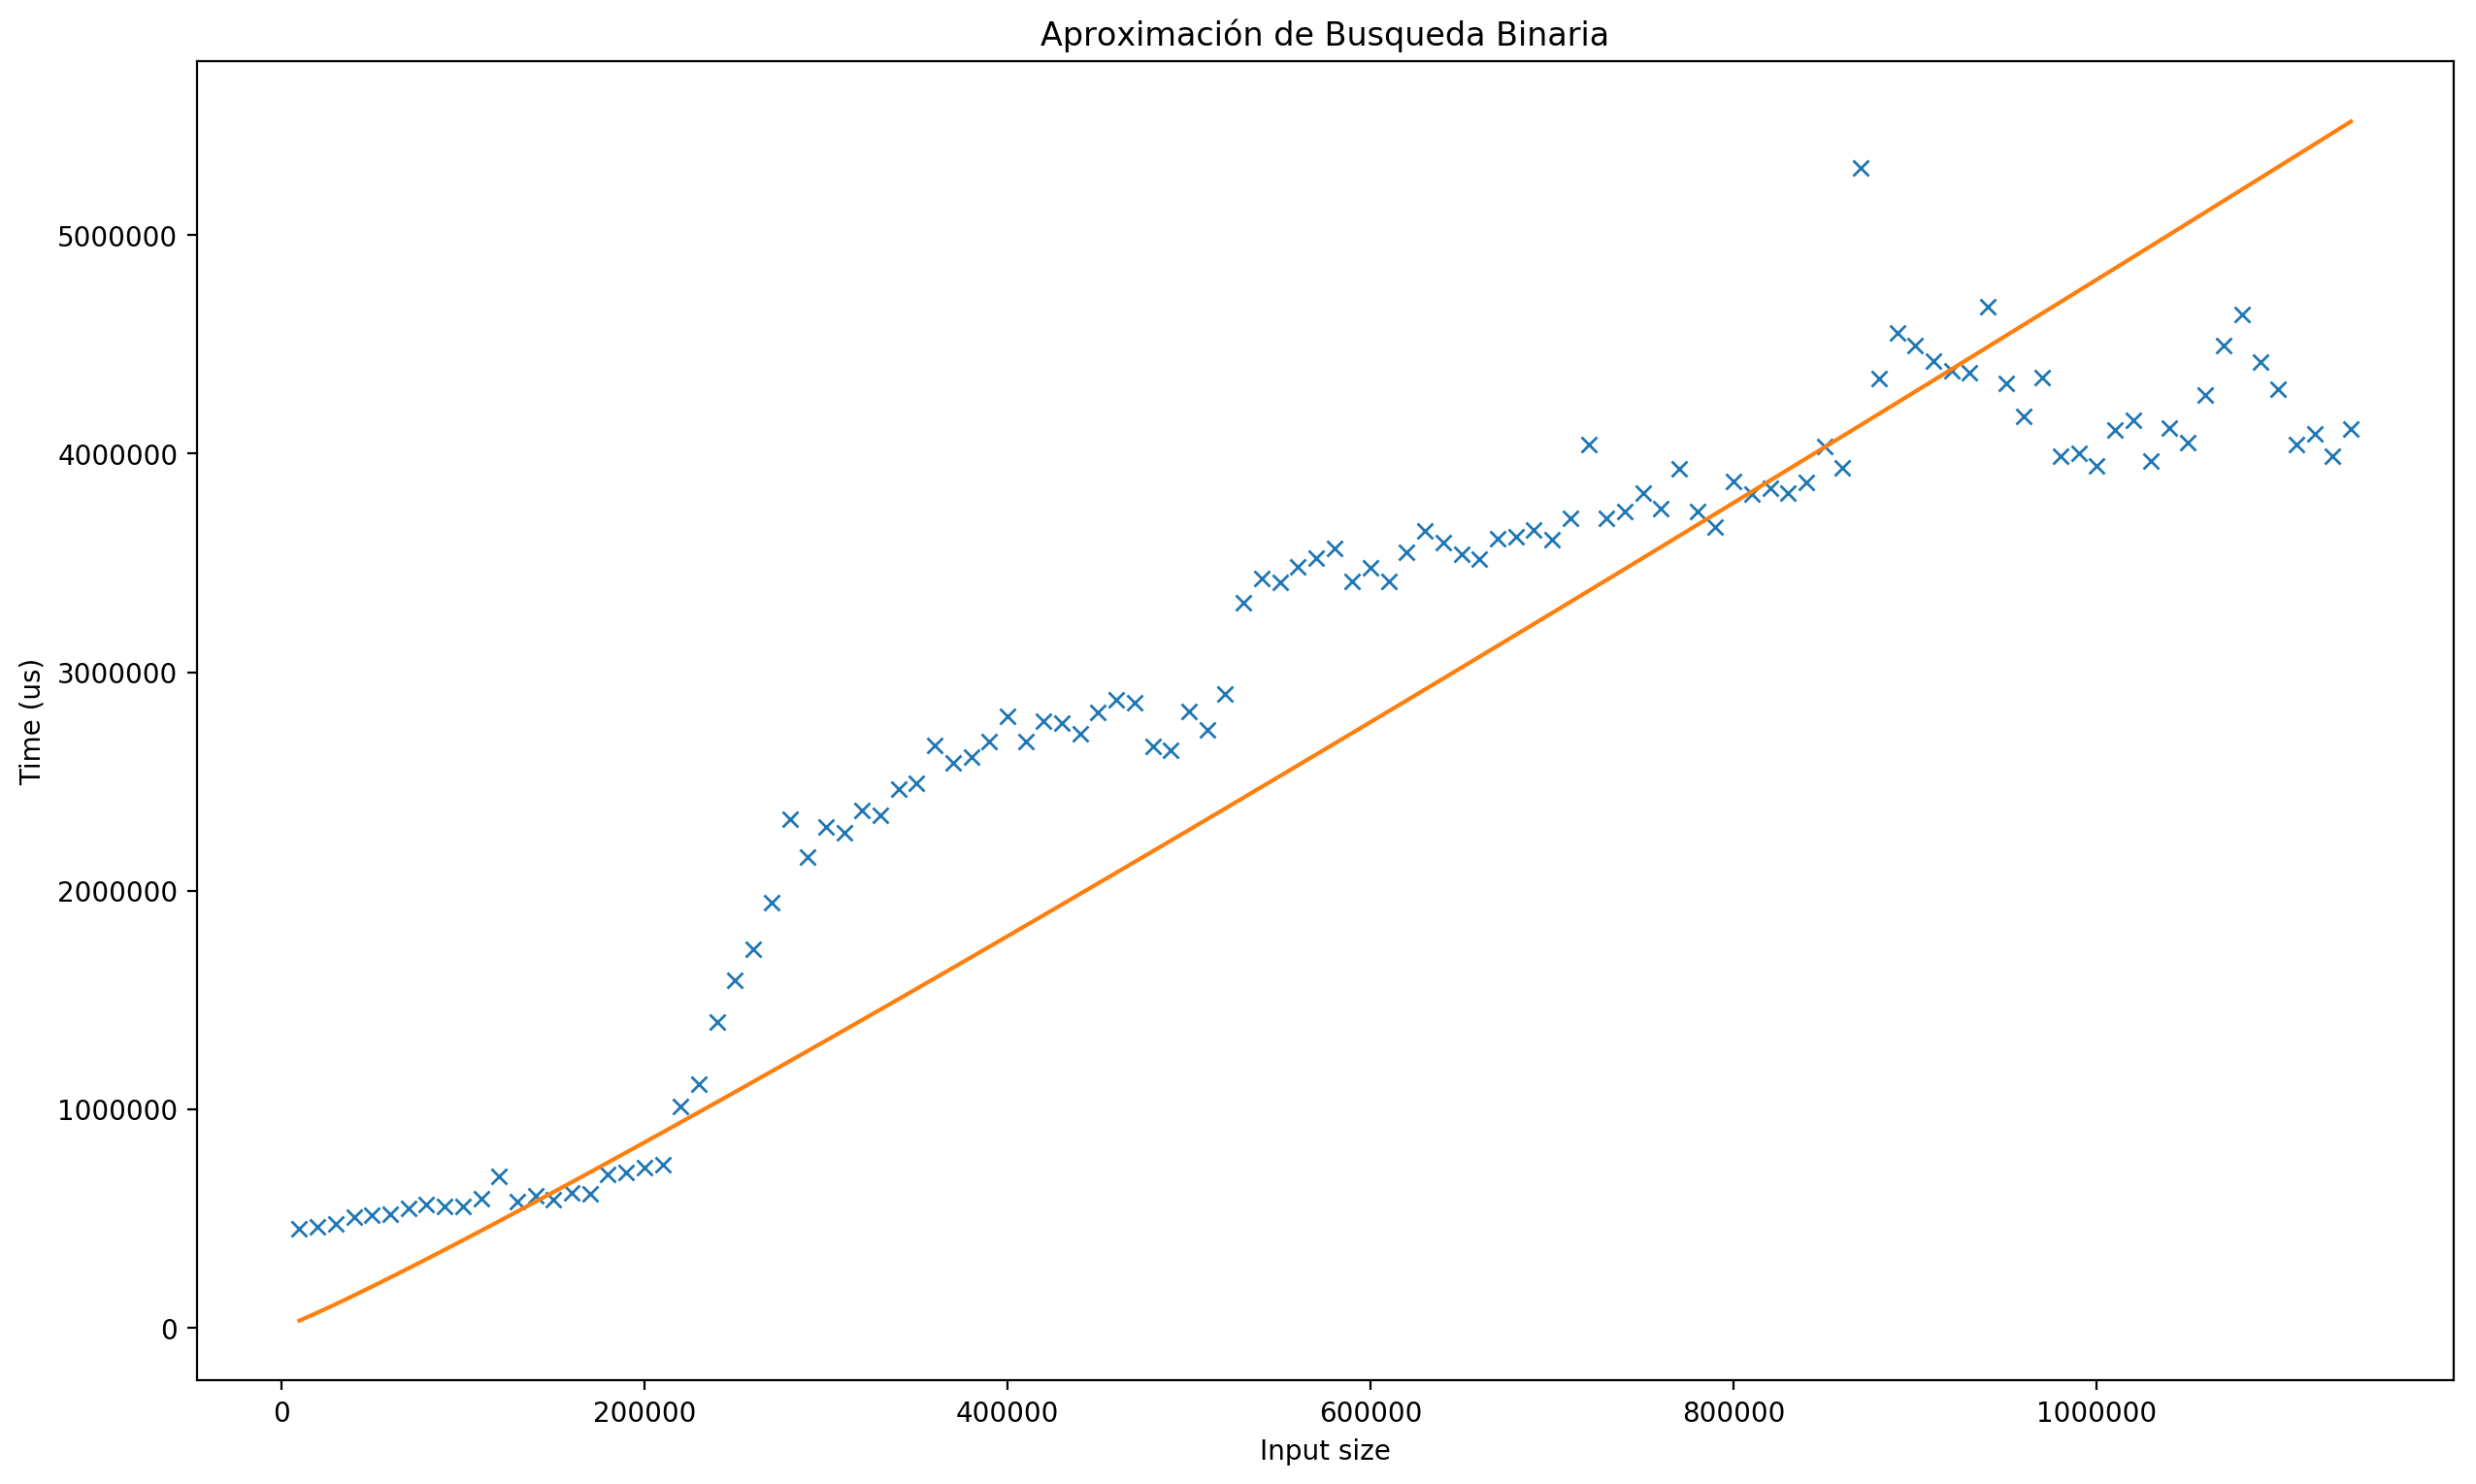
\includegraphics[width=15cm]{./Graficas/busquedabinaria_ajuste.png}
	\end{center}	
\end{datos}

Realizamos con \emph{Jupyter} el ajuste de regresión para obtener la siguiente función:
$$T(n)=0.28166261 \cdot n\log n$$

Es importante notar que, en este algoritmo, los datos han salido más dispersos, gracias a su gran velocidad. Debido a esto, hemos tenido que realizar varias pruebas para obtener datos con cierta validez.

En este caso, el mejor error posible lo tiene la recta, esto puede ser así debido a la perturbación de los datos, o al hecho de que $n\log n$ es muy similar a $n$. A continuación, aparece la relación entre los errores encontrados entre el resto de funciones aproximables (el que tiene mayor error tiene el 100\%, y de ahí los porcentajes restantes son los errores relativos a éste):

\begin{itemize}
	\item \textbf{Error para recta ($kn$): 7.227564149512647\%}
	\item Error para cuadrática ($kn^2$): 56.14209694786215\%
	\item Error para cúbica ($kn^3$): 74.09603399513483\%
	\item Error para logarítmica ($k\log n$): 100.0\%
	\item \textbf{Error para $\boldsymbol{n}$-logarítmica ($\boldsymbol{kn\log n}$): 13.766671701121327\%}
\end{itemize}

\section{Algoritmo Heap Sort}

\begin{lstlisting}[language=C]
void heapsort(int T[], int num_elem) {
	for ( int i = num_elem/2; i >= 0; i-- ) {
		reajustar(T, num_elem, i);
	}
	for ( int i = num_elem-1; i >= 1; i-- ) {
		int aux = T[0];
		T[0] = T[i];
		T[i] = aux;
		reajustar(T, i, 0);
	}
}
\end{lstlisting}

\begin{lstlisting}[language=C]
void reajustar(int T[], int num_elem, int k) {
	int j, v = T[k];
	bool esAPO = false;
	
	while ( ( k < num_elem/2 ) && !esAPO ) {
		j = 2*k + 1;
		if ( ( j < ( num_elem - 1 ) ) && ( T[j] < T[j+1] ) )
			j++;
		if ( v >= T[j] )
			esAPO = true;
			T[k] = T[j];
			k = j;
	}
	
	T[k] = v;
}
\end{lstlisting}

\subsection{Eficiencia teórica}

Podemos observar que en la función principal \texttt{heapsort} se hace una llamada a la función \texttt{reajustar}, por lo que, primeramente, vamos a estudiar la eficiencia de esta función.

\subsubsection*{Estudio de la función \texttt{reajustar}}

En la función \texttt{reajustar} llamaremos $n$ al tamaño del vector, en este caso es la variable \texttt{num\_elem}. Las cuatro primeras operaciones son $O(1)$, lo que nos lleva a estudiar el bucle \texttt{while} para el cálculo de la eficiencia del algoritmo. Como podemos observar en la \emph{línea 2}, la variable \texttt{k} es un índice del vector, lo que implica que $0 \leq \texttt{k} \leq n-1$. El peor caso de ejecución será en el que el bucle haga el mayor número de iteraciones, para ello $\texttt{k} < \frac{n}{2}$ el mayor número de veces posible, para que esto se cumpla \texttt{k} ha de incrementar lo mínimo posible en cada iteración. En el código vemos que al final del bucle \texttt{k} se iguala a \texttt{j}, como hemos dicho anteriormente queremos que \texttt{k} incremente de forma mínima, por lo que suponemos que el primer \texttt{if} (con eficiencia $O(1)$) no se cumple ya que incrementa la \texttt{j} y al final repercute en el aumento de la \texttt{k}. También, para que el número de iteraciones sea máxima, el segundo \texttt{if} no ha de cumplirse porque al cambiar \texttt{esAPO}, saldría del bucle.

A partir de todo esto podemos observar que $k_{i} = 2k_{i-1} + 1$, siendo $i$ el número de la iteración. Obtenemos así una recurrencia que procedemos a resolver:
$$k_i = 2^i \cdot c$$
Con la solución particular:
\begin{align*}
x &= 2x +1 \\
x &= -1
\end{align*}
Obteniendo como solución de la recurrencia:
$$k_i = 2^i \cdot c -1$$
Como queremos que haga el número máximo de iteraciones y $0 \leq \texttt{k} \leq n-1$, necesitamos que \texttt{k} esté ``lo más alejado posible'' de $\frac{n}{2}$ por lo que suponemos que la \texttt{k} inicial vale 0, es decir, $\text{\texttt{k}}_0 = 0$, por lo que
\begin{align*}
k_0 &= 2^0 \cdot c -1\\
0 &= 1 \cdot c -1\\
c &= 1
\end{align*}

Obtenemos así la solución de la recurrencia: $$k_i = 2^i -1$$
Para ver el número máximo de iteraciones tenemos que ver en qué $i$ de la iteración es $k = \frac{n}{2}$.
\begin{align*}
2^i - 1 &= \frac{n}{2}\\
2^i &= \frac{n-2}{2}\\
i &= \log_2{\frac{n-2}{2}}\\
i&=\log_2(n-2) - \log_2{2}\\
i&=\log_2(n-2) -1
\end{align*}
Con todo lo dicho, el cuerpo del \texttt{while} tiene una eficiencia $O(log_2{n})$, y al ejecutar el bucle $n$ veces, tenemos que: $$T(n) \in O(\log n)$$


Habiendo estudiado la eficiencia de reajustar pasamos a estudiar la eficiencia del \texttt{heapsort}. Lo más relevante del código son los dos \texttt{for} , en el interior de ambos la eficiencia es la de la función \texttt{reajustar}, ya que el resto de operaciones son $O(1)$, el primer \texttt{for} se ejecuta $\frac{n}{2}$ veces, siendo n el tamaño del vector, y el segundo \texttt{for} se ejecuta $n-1$ veces, por lo que la eficiencia del algoritmo es $O((n-1)\log_2{n}) \equiv \boldsymbol{O(n\log{n})}$.

\subsection{Eficiencia empírica}

Tras ejecutar el algoritmo con \texttt{num\_elem} desde $10000$ hasta $100000$ en tramos de $10000$, y de ahí hasta $500000$ en tramos de $50000$; los resultados de ejecución para cada uno de los miembros del grupo fueron los siguientes:

\begin{datos}\hspace{-0.2cm}
	{\bf\sffamily Gráfico 5.1.} {\sffamily Datos de todas las ejecuciones}\\
	\vspace{-0.7cm}
	\begin{center}
		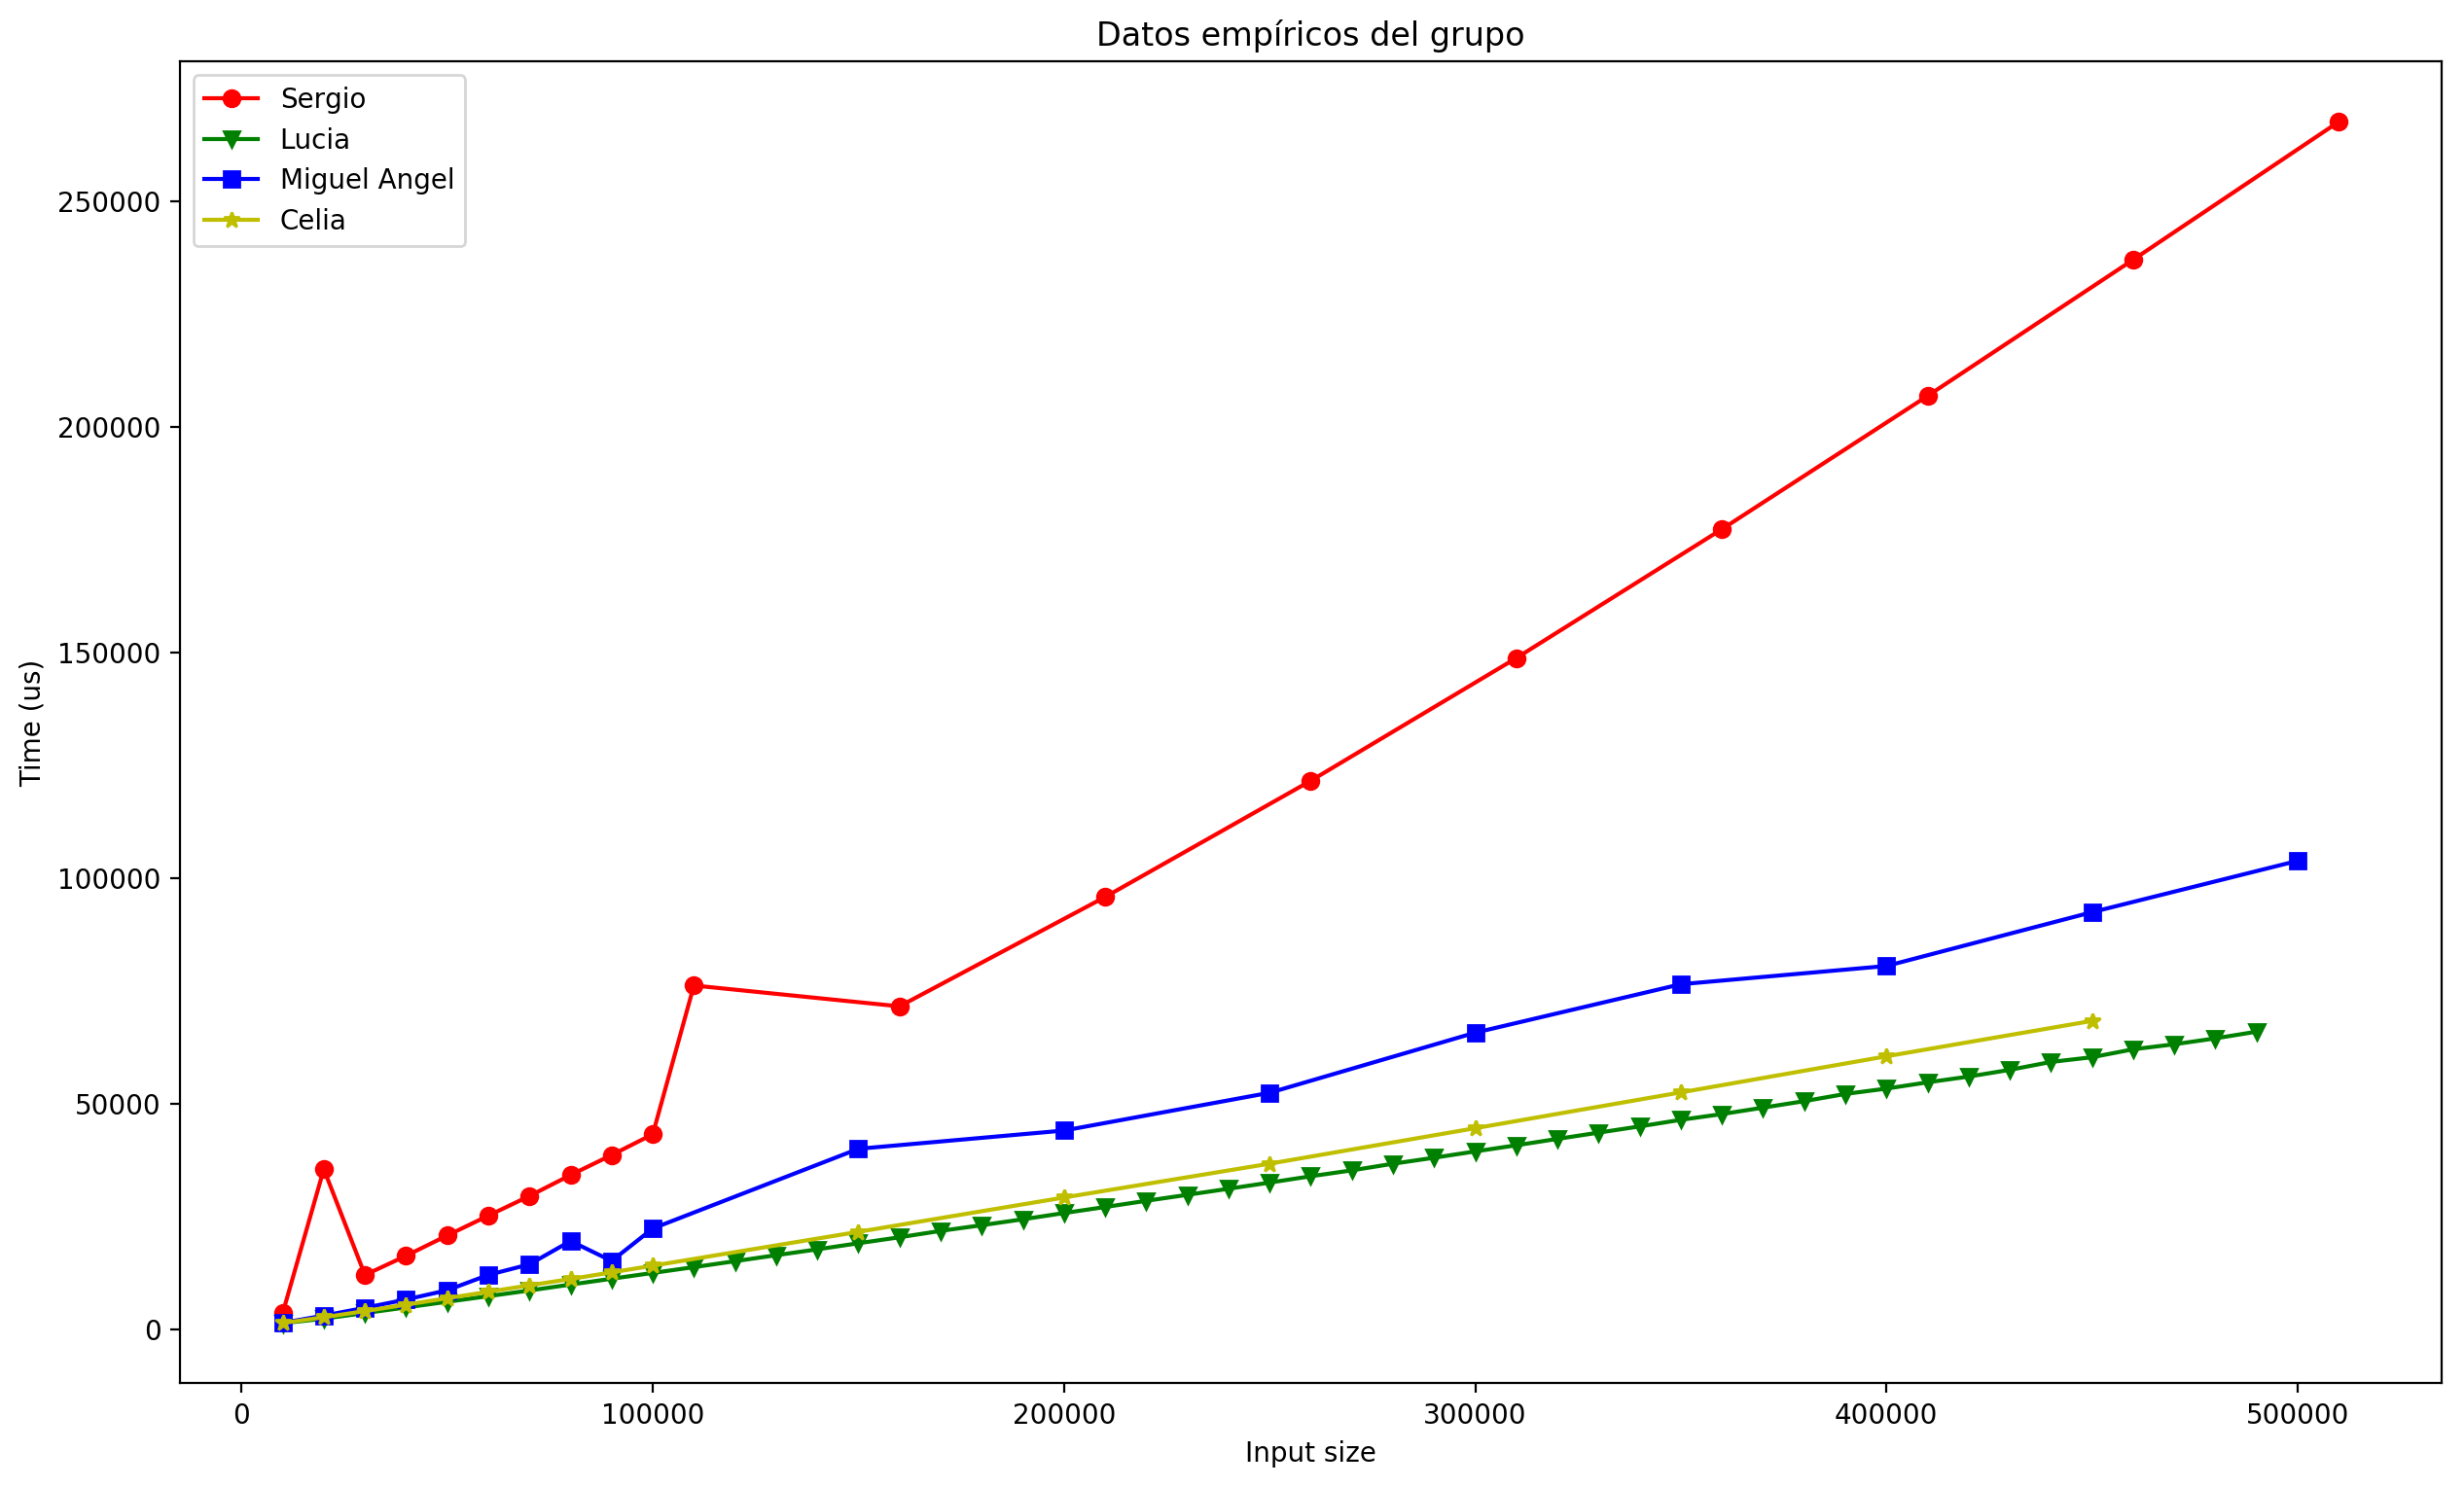
\includegraphics[width=15cm]{./Graficas/heap_todos.png}
	\end{center}
\end{datos}

\subsection{Eficiencia híbrida}

A través de la eficiencia híbrida, comprobaremos que el ajuste teórico realizado es correcto.

Para realizar el análisis de la eficiencia híbrida, tomamos las ejecuciones de uno de los integrantes.

\begin{datos}
	{\bf\sffamily Gráfico 5.2.} {\sffamily Datos que serán usados para el análisis híbrido}\\
	\vspace{-0.7cm}
	\begin{center}
		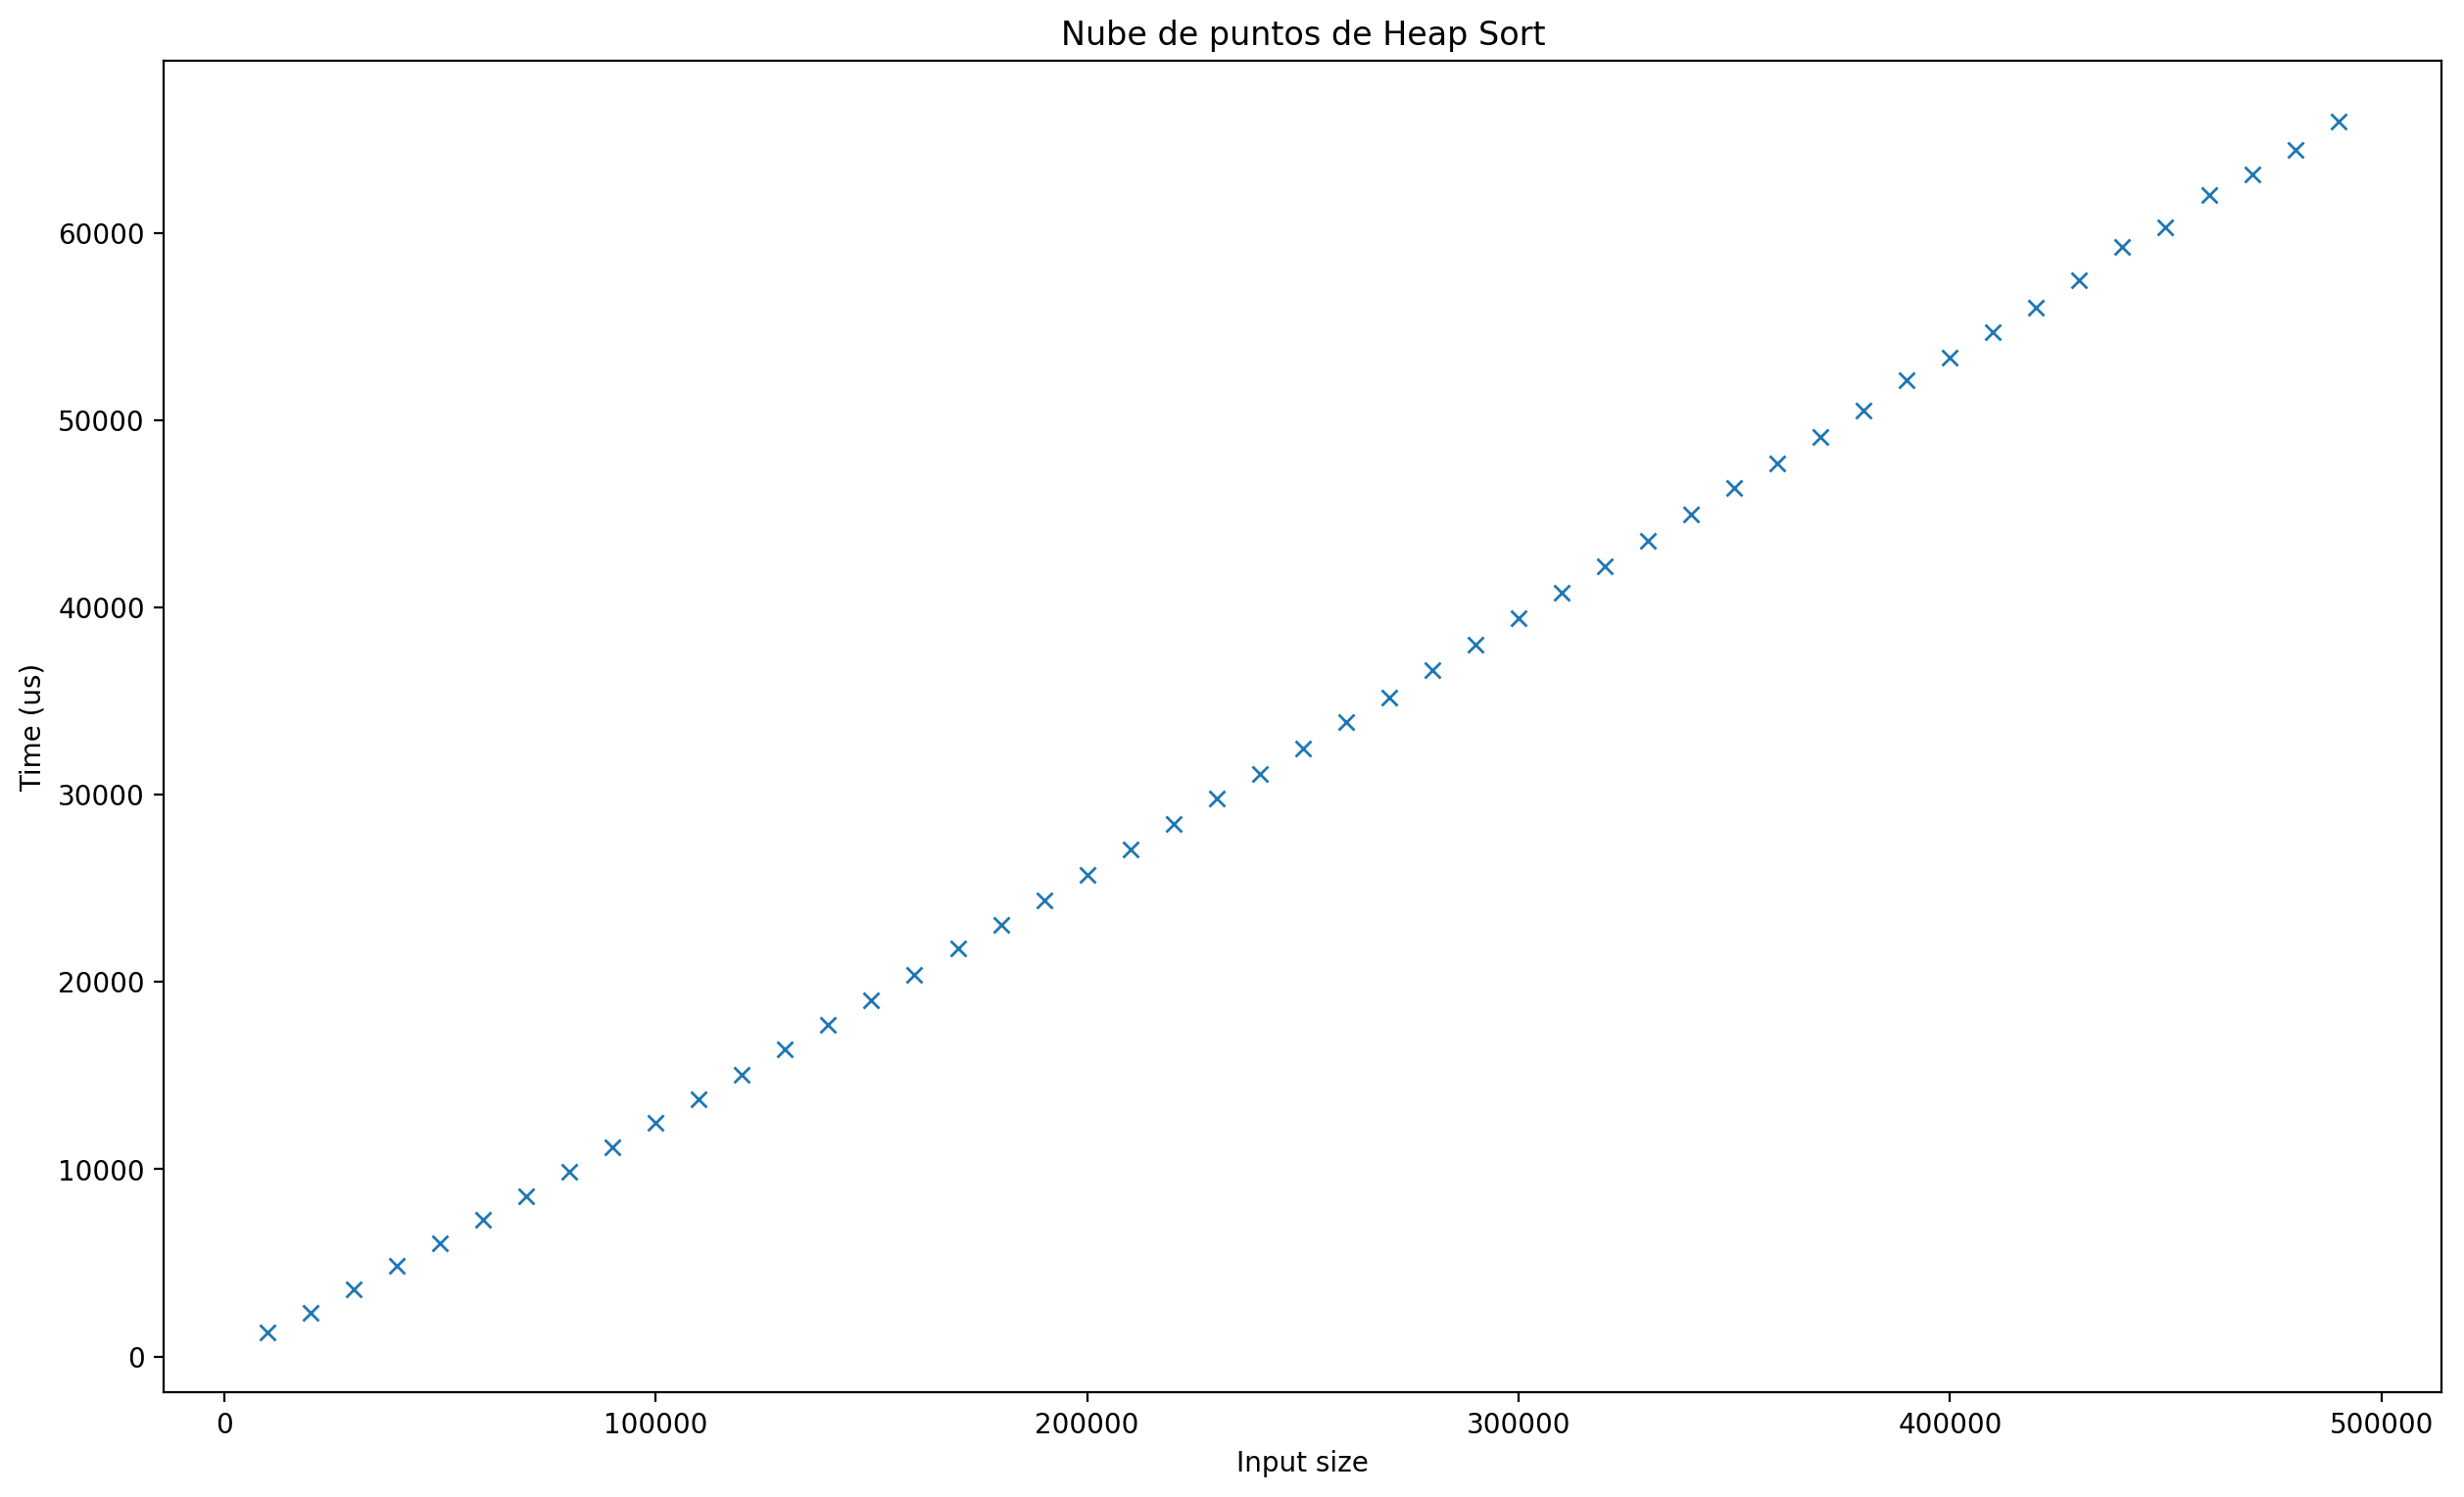
\includegraphics[width=15cm]{./Graficas/heap_nube.png}
	\end{center}	
\end{datos}

\subsubsection{Ajuste de constante oculta}

Tras realizar el ajuste de la constante oculta, el valor obtenido es de $K=0.9753044058661043$.
\pagebreak
\subsubsection{Ajuste por regresión}

\begin{datos}
	{\bf\sffamily Gráfico 5.3.} {\sffamily Ajuste por regresión}\\
	\vspace{-0.7cm}
	\begin{center}
		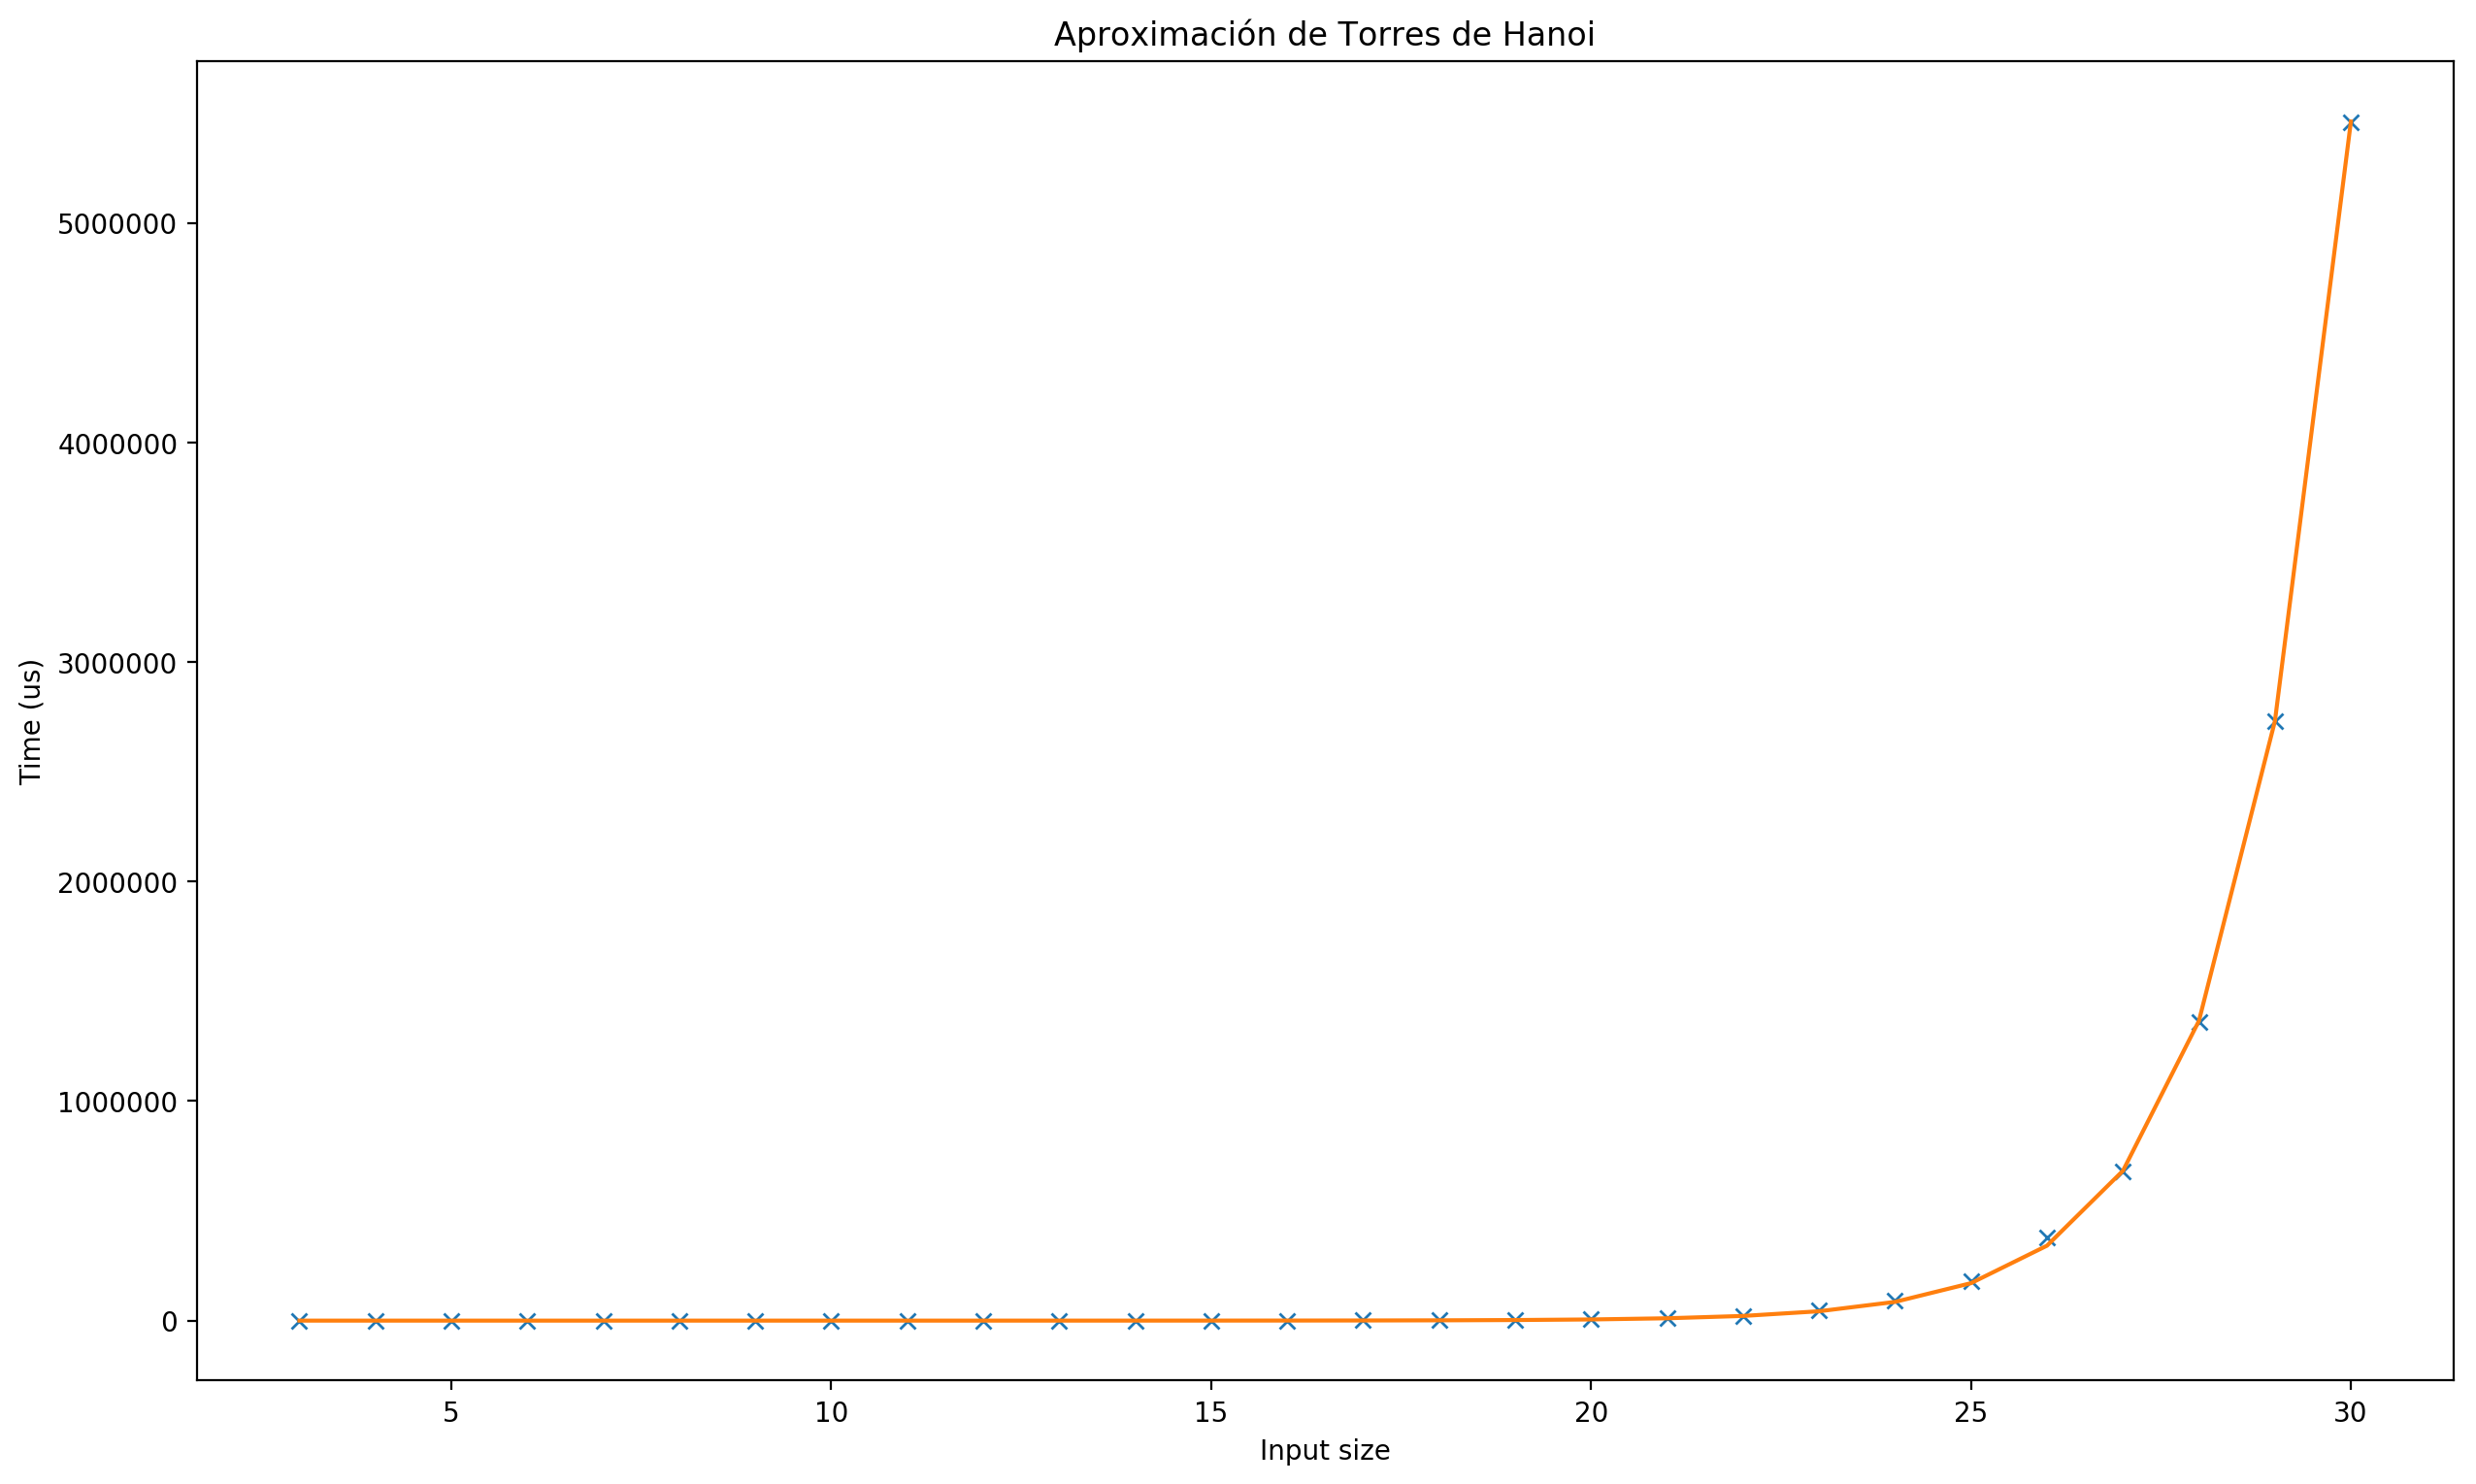
\includegraphics[width=15cm]{./Graficas/hanoi_ajuste.png}
	\end{center}	
\end{datos}

Realizamos con \emph{Jupyter} el ajuste de regresión para obtener la siguiente función:
$$T(n)=0.00718669\cdot n \log n$$

En este caso, el mejor error posible lo tiene la recta, esto puede ser así debido a la perturbación de los datos, o al hecho de que $n\log n$ es muy similar a $n$. A continuación, aparece la relación entre los errores encontrados entre el resto de funciones aproximables (el que tiene mayor error tiene el 100\%, y de ahí los porcentajes restantes son los errores relativos a éste):

\begin{itemize}
	\item \textbf{Error para recta ($kn$): 0.04033354197487824\%}
	\item Error para cuadrática ($kn^2$): 27.33530020306984\%
	\item Error para cúbica ($kn^3$): 74.09603399513483\%
	\item Error para logarítmica ($k\log n$): 100.0\%
	\item \textbf{Error para $\boldsymbol{n}$-logarítmica ($\boldsymbol{kn\log n}$): 0.04894682223025979\%}
\end{itemize}

\pagebreak
\section{Algoritmo Bubble Sort}

\begin{lstlisting}[language=C]
void burbuja(int v[], int n) {
	int aux;
	
	for ( int i = inicial, i < final-1; i++ ) {
		for ( j = final-1; j > i; j-- ) {
			if ( v[j] < v[j-1] ) {
				aux = v[j];
				v[j] = v[j-1];
				v[j-1] = aux;
			}
		}
	}
}
\end{lstlisting}

\subsection{Eficiencia teórica}


Este algoritmo es iterativo, por lo que nos centraremos en el estudio de los bucles \texttt{while} y \texttt{for} anidados que se encuentran en el código.

En las \emph{líneas 6-10}, vemos que las operaciones del bloque condicional son $O(1)$. Comenzaremos estudiando los bucles de dentro hacia afuera, para ello, llamaremos $n$ al tamaño del vector.

Estudiaremos el bucle \texttt{for} de la \emph{línea 5}. Este bucle se ejecuta de acuerdo a un $\texttt{i}$ fijado por el bucle \texttt{for} más externo \emph{línea 4}: desde $\texttt{fin}-1$ hasta $\texttt{i}$, en decrementos de $1$. Esto se ejecutará tantas veces como dicta el \texttt{for} más externo: desde $0$ hasta $\texttt{final}-2$. En definitiva, tenemos que:

$$ T(n) = \sum_{i=0}^{n-1}\left(n-i-1\right) = n^2 - \frac{(n-2)(n-1)}{2} - 5 \in O(n^2) $$

Por tanto, este algoritmo es $\boldsymbol{O(n^2)}$.

\subsection{Eficiencia empírica}

Tras ejecutar el algoritmo con \texttt{n} desde $10000$ hasta $100000$ en tramos de $10000$, y de ahí hasta $500000$ en tramos de $50000$; los resultados de ejecución para cada uno de los miembros del grupo fueron los siguientes:
\pagebreak
\begin{datos}\hspace{-0.2cm}
	{\bf\sffamily Gráfico 6.1.} {\sffamily Datos de todas las ejecuciones}\\
	\vspace{-0.7cm}
	\begin{center}
		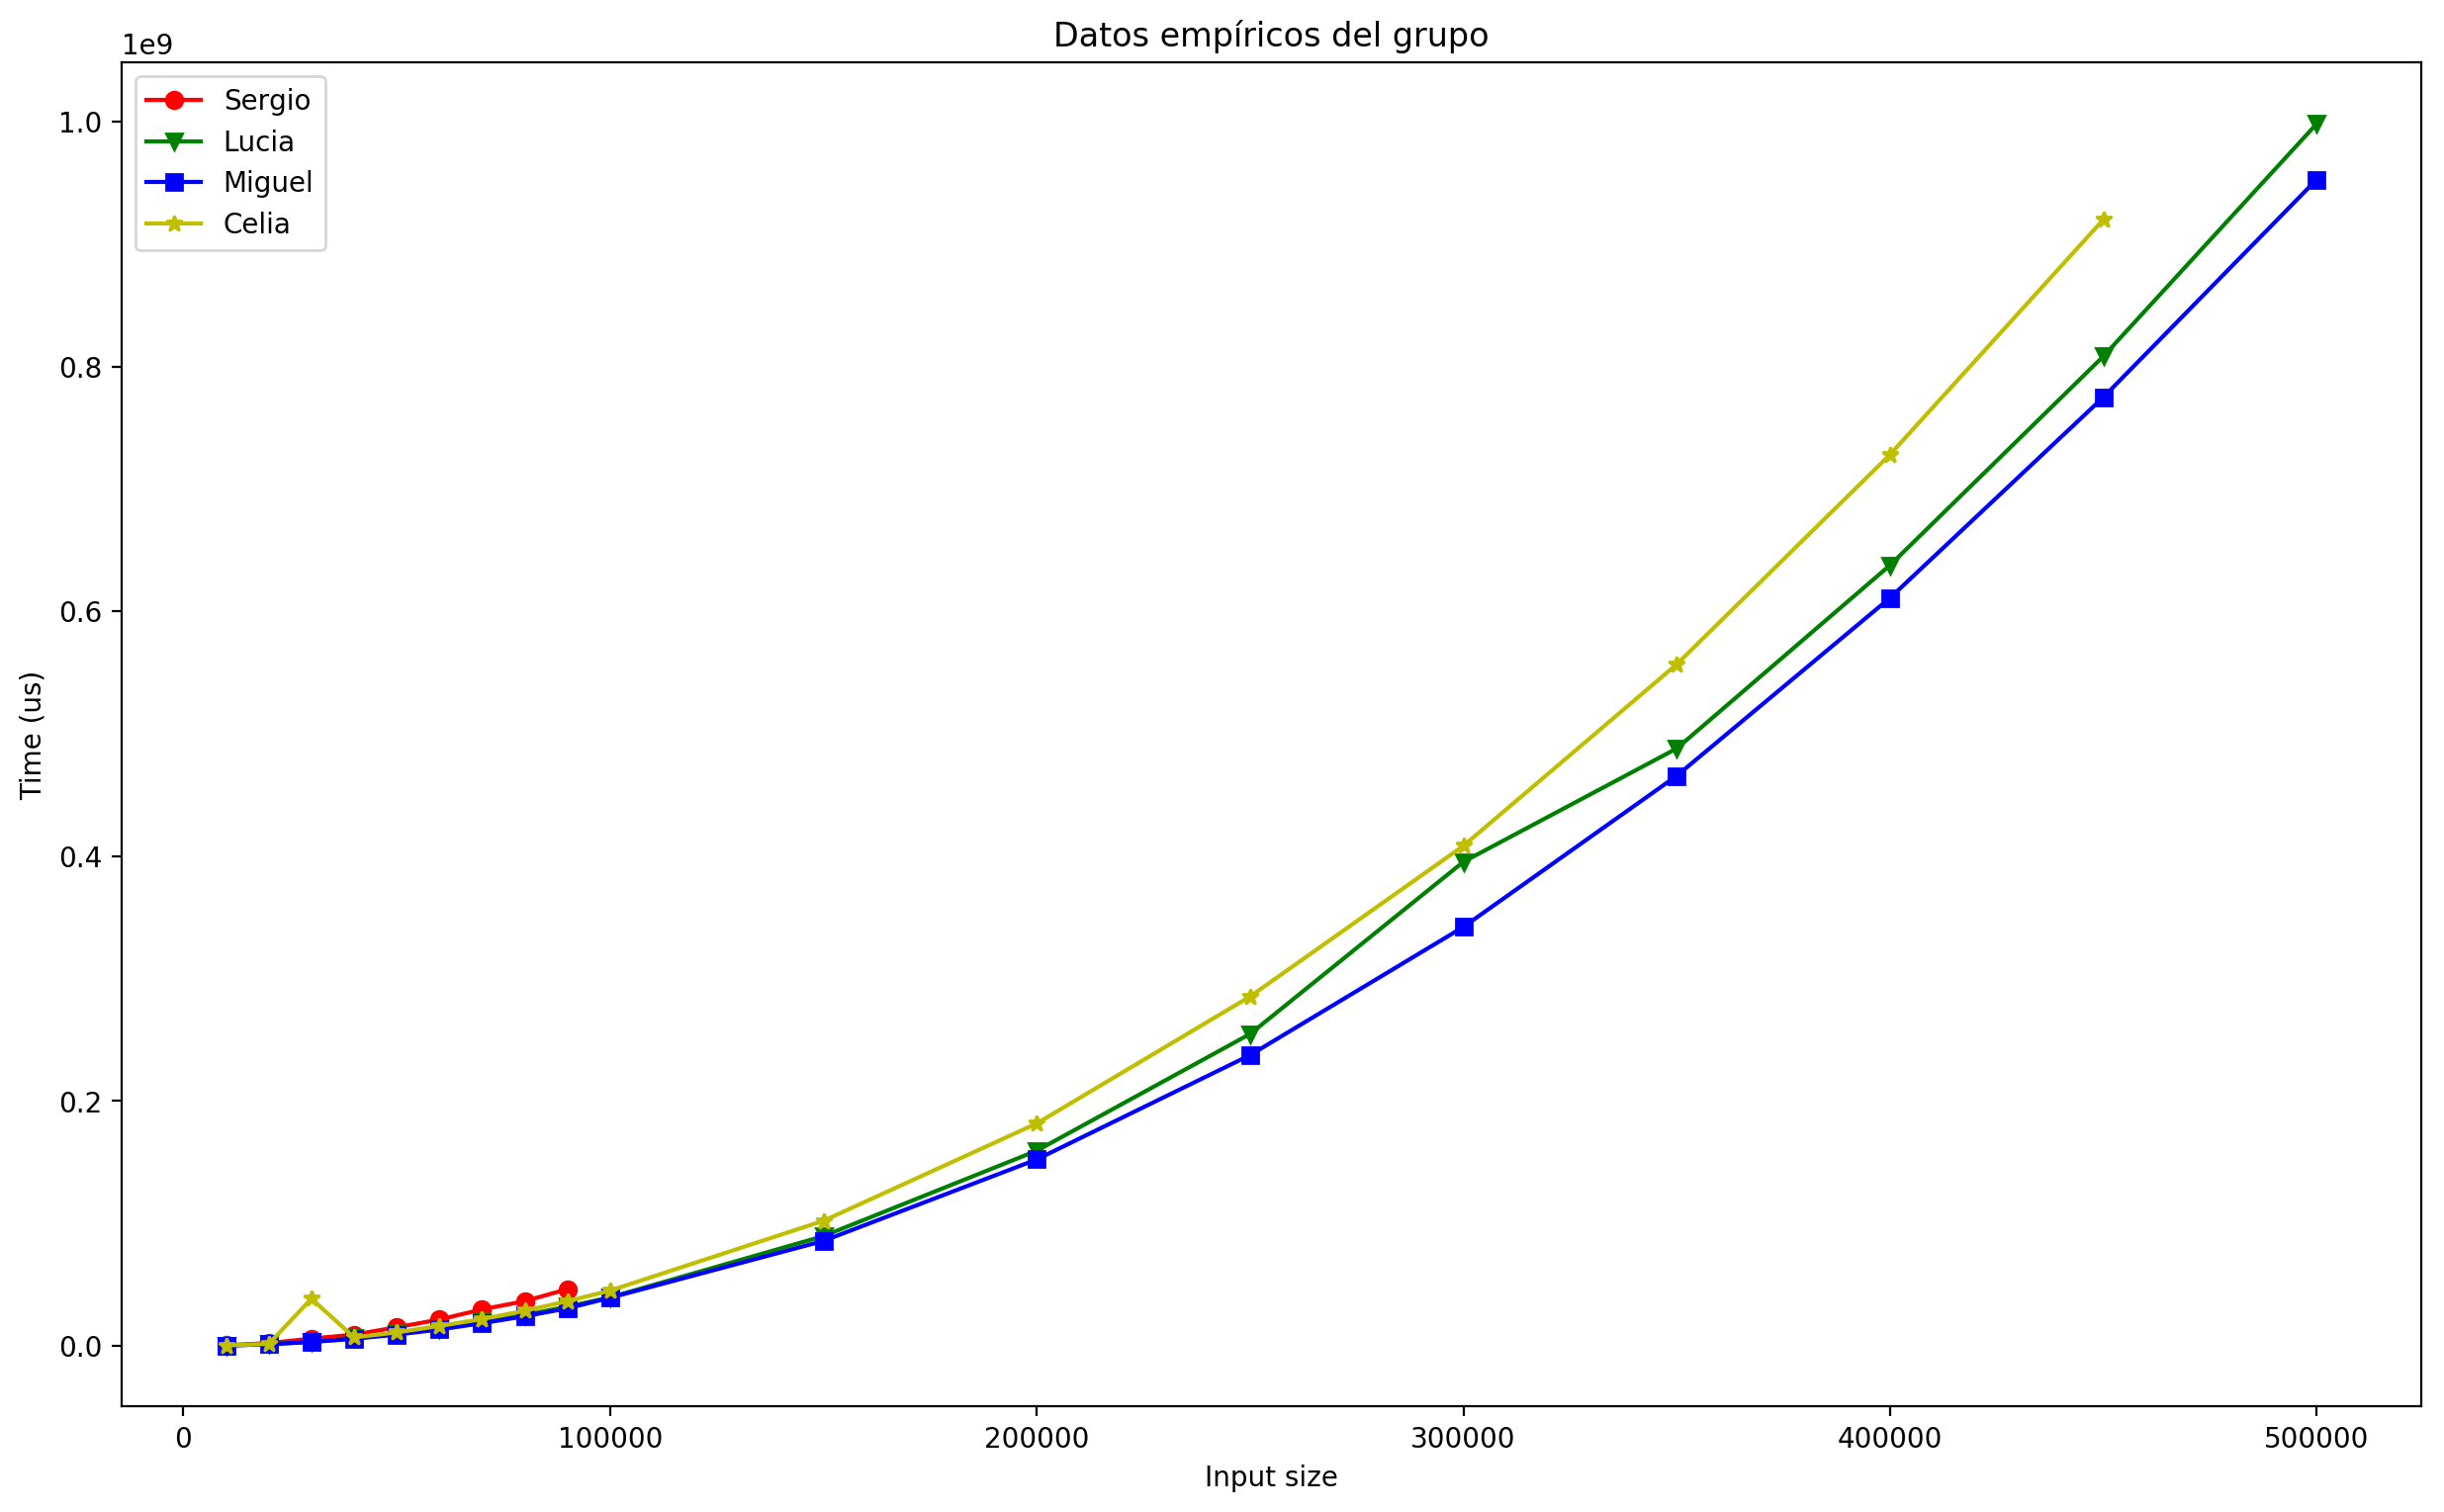
\includegraphics[width=15cm]{./Graficas/bubble_todos.png}
	\end{center}
\end{datos}

\subsection{Eficiencia híbrida}

A través de la eficiencia híbrida, comprobaremos que el ajuste teórico realizado es correcto.

Para realizar el análisis de la eficiencia híbrida, tomamos las ejecuciones de uno de los integrantes.

\pagebreak

\begin{datos}
	{\bf\sffamily Gráfico 6.2.} {\sffamily Datos que serán usados para el análisis híbrido}\\
	\vspace{-0.7cm}
	\begin{center}
		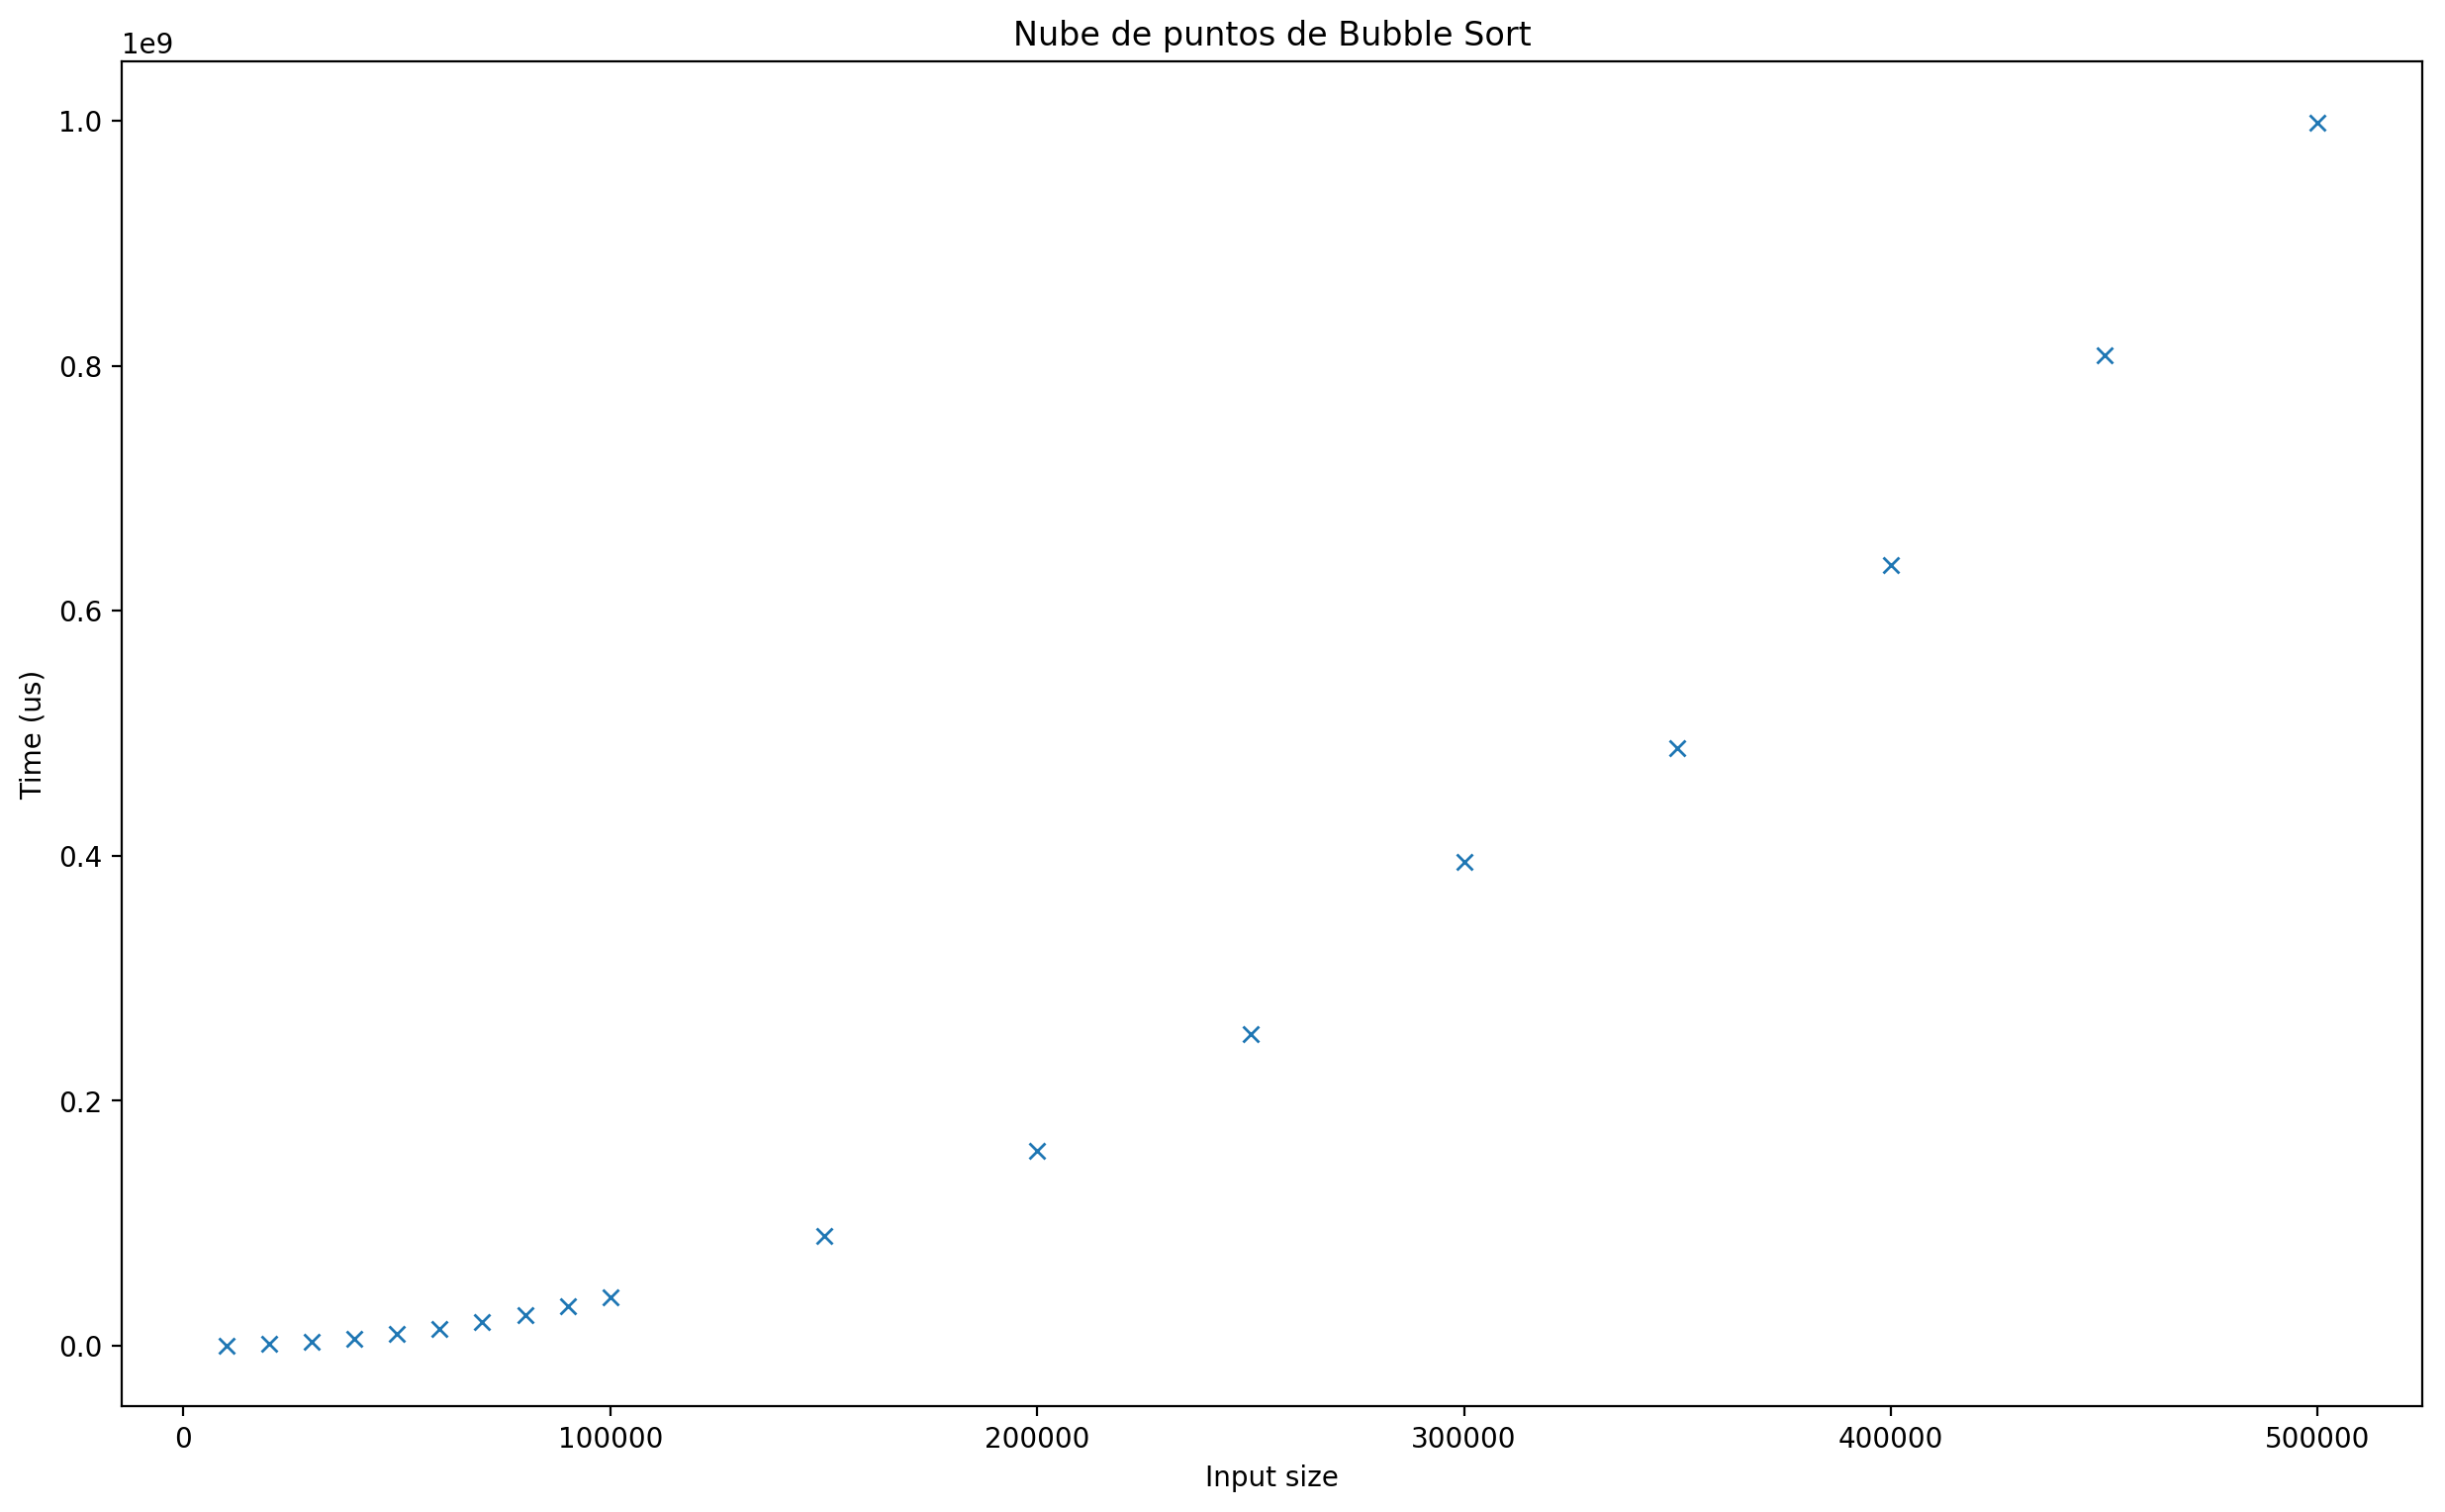
\includegraphics[width=15cm]{./Graficas/bubble_nube.png}
	\end{center}	
\end{datos}

\subsubsection{Ajuste de constante oculta}

Tras realizar el ajuste de la constante oculta, el valor obtenido es de $K=1.019659179330859$.
\pagebreak
\subsubsection{Ajuste por regresión}

\begin{datos}
	{\bf\sffamily Gráfico 6.3.} {\sffamily Ajuste por regresión}\\
	\vspace{-0.7cm}
	\begin{center}
		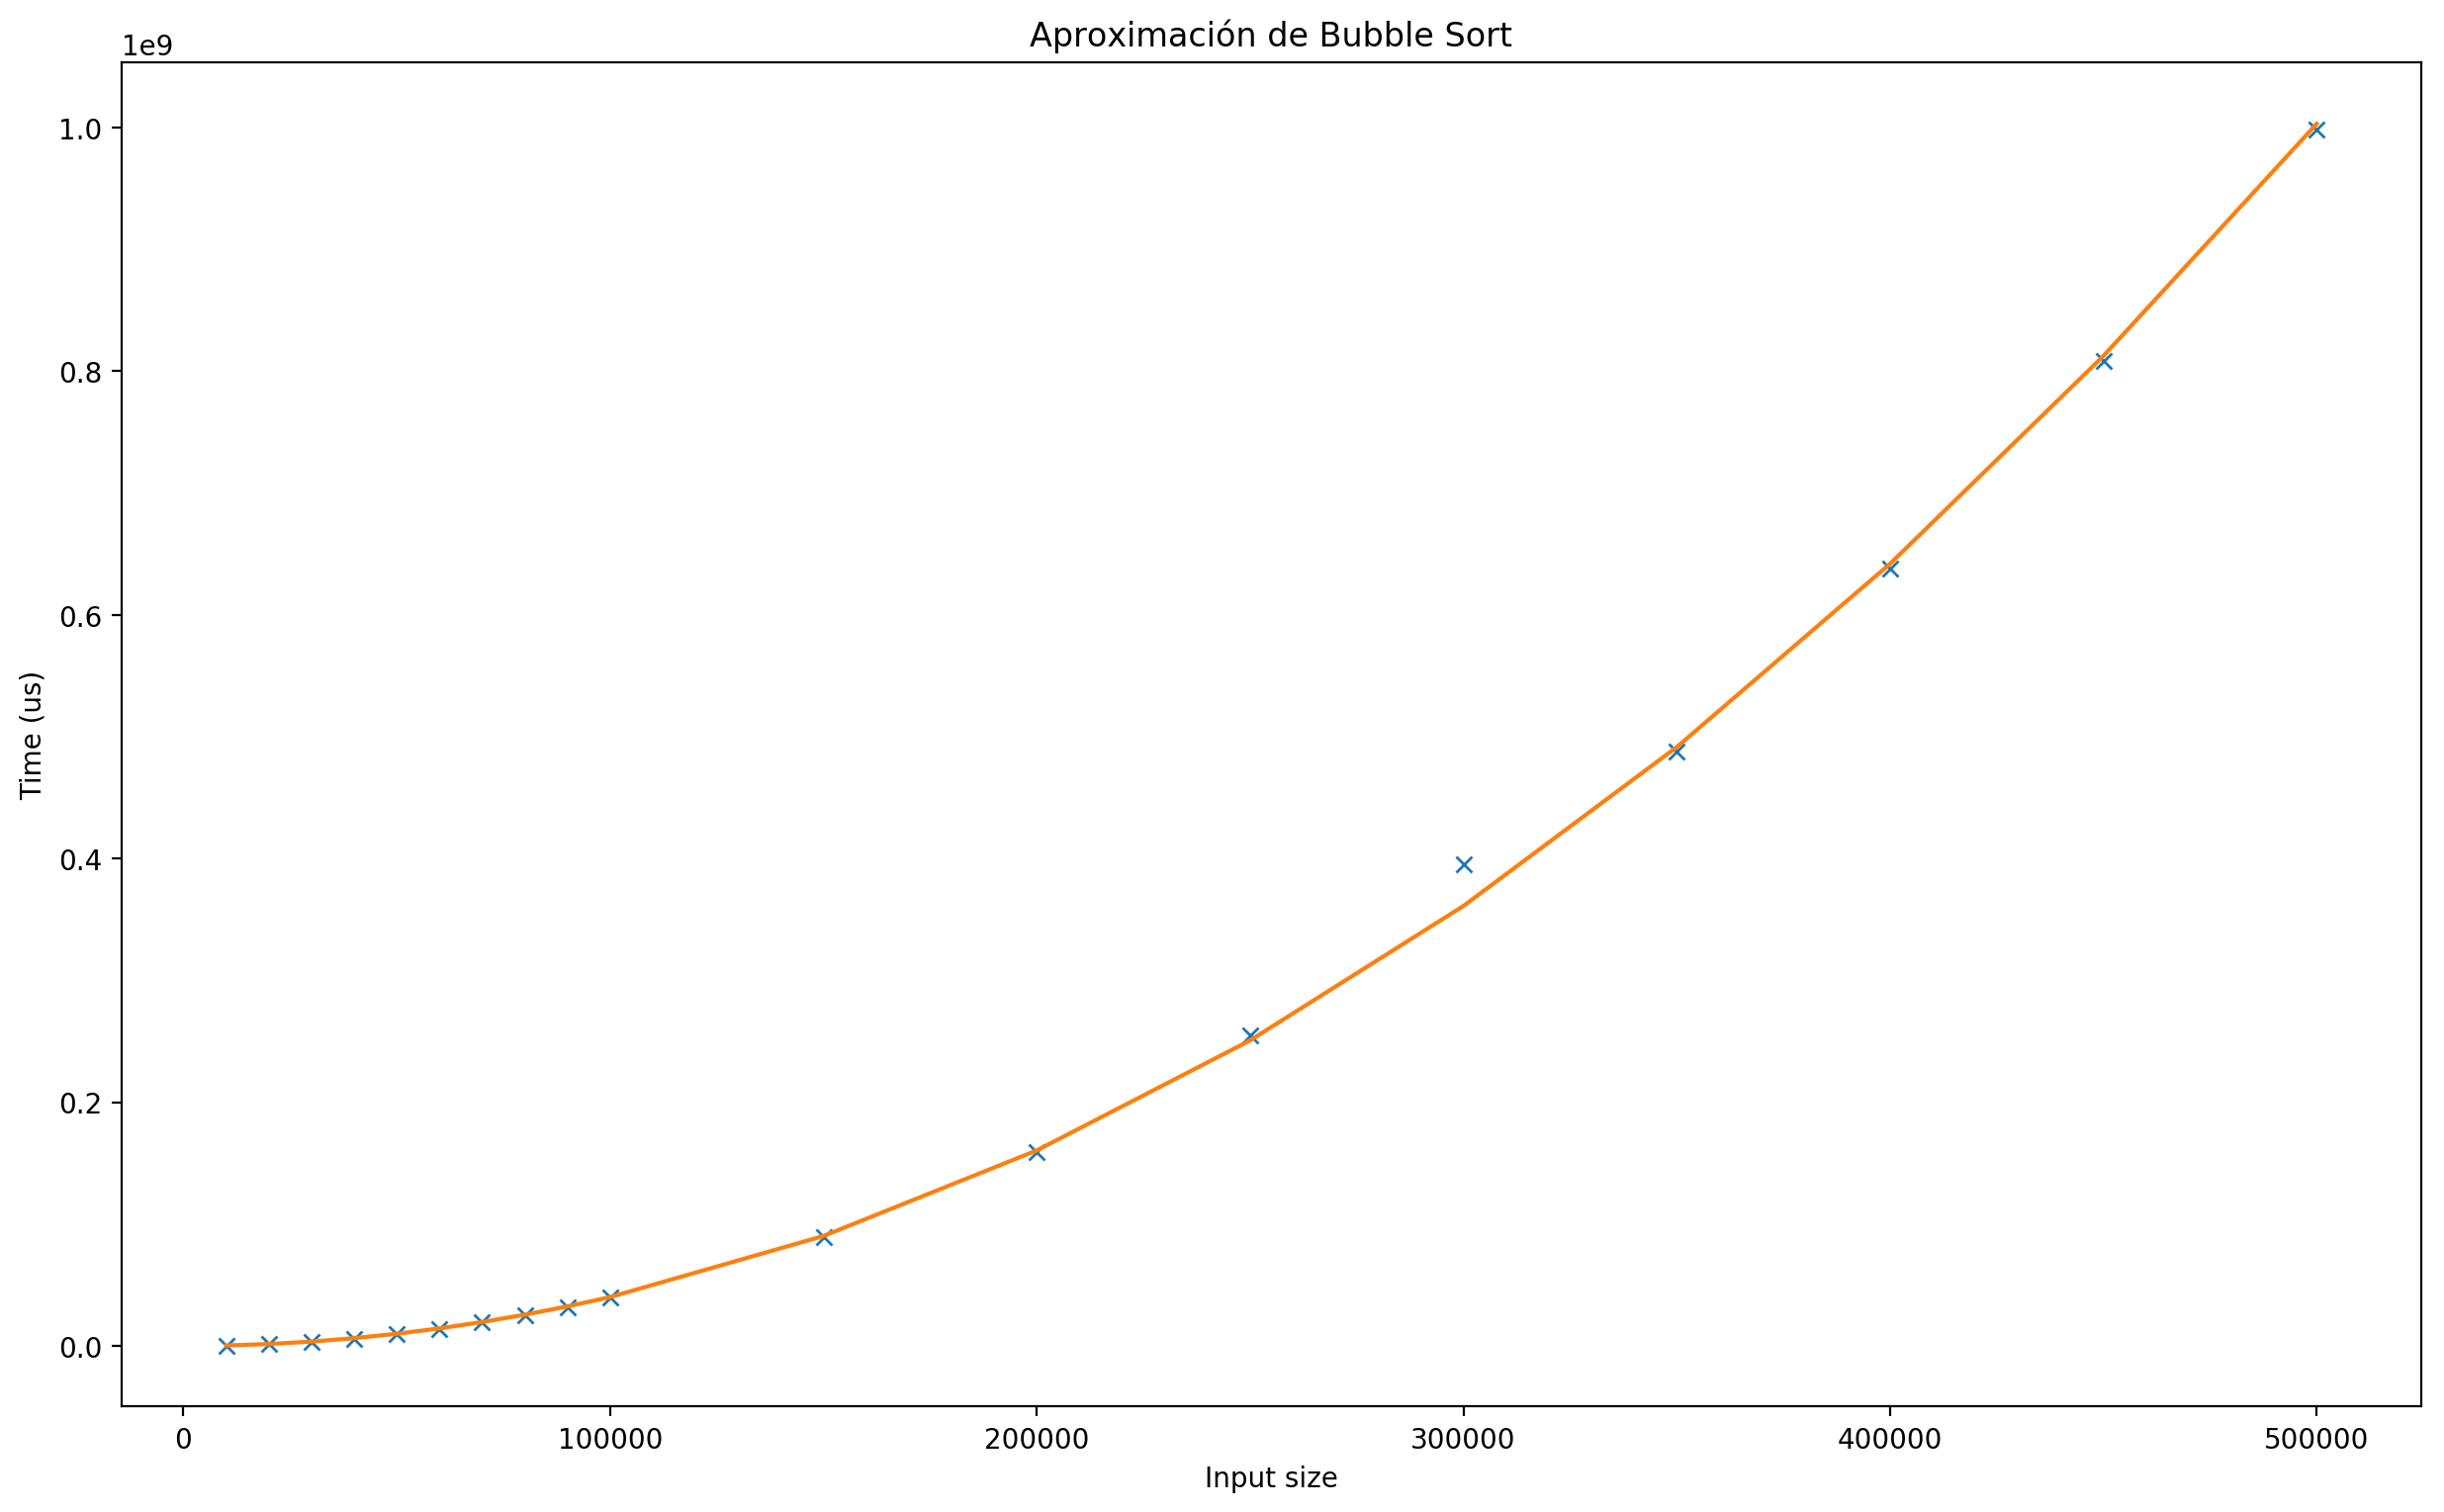
\includegraphics[width=15cm]{./Graficas/bubble_ajuste.png}
	\end{center}	
\end{datos}

Realizamos con \emph{Jupyter} el ajuste de regresión para obtener la siguiente función:
$$T(n)=0.00401246\cdot n^2$$

Que es la que mejor aproxima a nuestros datos. Nótese que es quien tiene el mejor error posible de entre el resto de funciones aproximables (el que tiene mayor error tiene el 100\%, y de ahí los porcentajes restantes son los errores relativos a éste):

\begin{itemize}
	\item Error para recta ($kn$): 6.15853318137504\%
	\item \textbf{Error para cuadrática ($kn^2$): 0.08527050249560174\%}
	\item Error para cúbica ($kn^3$): 5.41027219494451\%
	\item Error para logarítmica ($k\log n$): 100.0\%
	\item Error para $n$-logarítmica ($kn\log n$): 10.096552530276018\%
\end{itemize}
\pagebreak
\section{Algoritmo Merge Sort}

\begin{lstlisting}[language=C++] 
static void mergesort_lims(int T[], int inicial, int final) {
	if ( final-inicial < UMBRAL_MS ) {
		insercion_lims(T, inicial, final);
	} else {
		int k = (final - inicial)/2;

		int * U = new int [k - inicial + 1];
		assert(U);
		int l, l2;
		for (l = 0, l2 = inicial; l < k; l++, l2++)
			U[l] = T[l2];
		U[l] = INT_MAX;

		int * V = new int [final - k + 1];
		assert(V);
		for (l = 0, l2 = k; l < final - k; l++, l2++)
			V[l] = T[l2];
		V[l] = INT_MAX;

		mergesort_lims(U, 0, k);
		mergesort_lims(V, 0, final - k);
		fusion(T, inicial, final, U, V);
		delete [] U;
		delete [] V;
	}
}
\end{lstlisting}
\begin{lstlisting}[language=C]
static void fusion(int T[], int inicial, int final, int U[], int V[]) {
	int j = 0, k = 0;
	for ( int i = inicial; i < final; i++ ) {
		if (U[j] < V[k]) {
			T[i] = U[j];
			j++;
		} else {
			T[i] = V[k];
			k++;
		}
	}
}
\end{lstlisting}

\subsection{Eficiencia teórica}

Sabemos que el algoritmo de inserción es $O(n^2)$, pero solo se ejecutará si el tamaño del vector es suficientemente pequeño. Estudiaremos el caso contrario.

Lo primero que hace es dividir el vector en dos partes iguales. Las instrucciones de las \emph{líneas 5-9, 12-15 y 18} son $O(1)$ y los dos bucles \texttt{for} se repiten cada uno $\frac{\texttt{k}}{2}$, por tanto llegado a este punto tenemos eficiencia $O(n)$. En las \emph{líneas 20 y 21} hacemos dos llamadas recursivas a \texttt{mergesort\_lims} y en la \emph{línea 22} llamamos a \texttt{fusion}. Estudiaremos estos dos hechos por separado.

\subsubsection*{Estudio de la función \texttt{fusion}}
La función \texttt{fusion}, por un lado, tiene un bucle \texttt{for} que se ejecuta $n$ veces. Las demás instrucciones son $O(1)$, por tanto, podemos decir que su eficiencia es $O(n)$.

\subsubsection*{Estudio de la función \texttt{mergesort\_lims}}

Las dos llamadas recursivas a \texttt{mergesort\_lims} se hacen sobre vectores que constituyen cada uno la mitad del vector original. Construimos la ecuación de recurrencia teniendo en cuenta todo lo anteriormente especificado, y sólo el caso $n \geq \texttt{UMBRALMS}$.
$$ T(m) = 2T(\frac{m}{2}) +n $$
Sustituyendo $m$ por $2^k$  y despejando obtenemos:
$$ T(2^k) - 2T(2^{k-1} ) = 2^k $$
Resolvemos la recurrencia:
\begin{align*}
(x-2) * (x-2) &= 0\\
(x-2)^2 &= 0
\end{align*}
\begin{align*}
t_{k} &= c_{1}*2^k + c_{2}*k*2^k \\
t_{n} &= c_{1}*n+c_{2}*\log_{2}(n)*n
\end{align*}

Tenemos que este algoritmo es $O(\log n)$.

\subsubsection*{Conclusión}

Por tanto deducimos que el algoritmo es $\boldsymbol{O(n\log_{2}(n))}$.

Hay que señalar que, si el tamaño del vector es suficientemente pequeño, el algoritmo sería $O(n^2)$ $-$al usar el algoritmo de inserción en ese caso$-$ pero no significará un retraso en los tiempos de ejecución ya que este algoritmo funciona bien para casos no demasiado grandes.

\subsection{Eficiencia empírica}

Tras ejecutar el algoritmo con un tamaño del vector variando desde $10000$ hasta $100000$ en tramos de $10000$, y de ahí hasta $500000$ en tramos de $50000$; los resultados de ejecución para cada uno de los miembros del grupo fueron los siguientes:
\pagebreak
\begin{datos}\hspace{-0.2cm}
	{\bf\sffamily Gráfico 7.1.} {\sffamily Datos de todas las ejecuciones}\\
	\vspace{-0.7cm}
	\begin{center}
		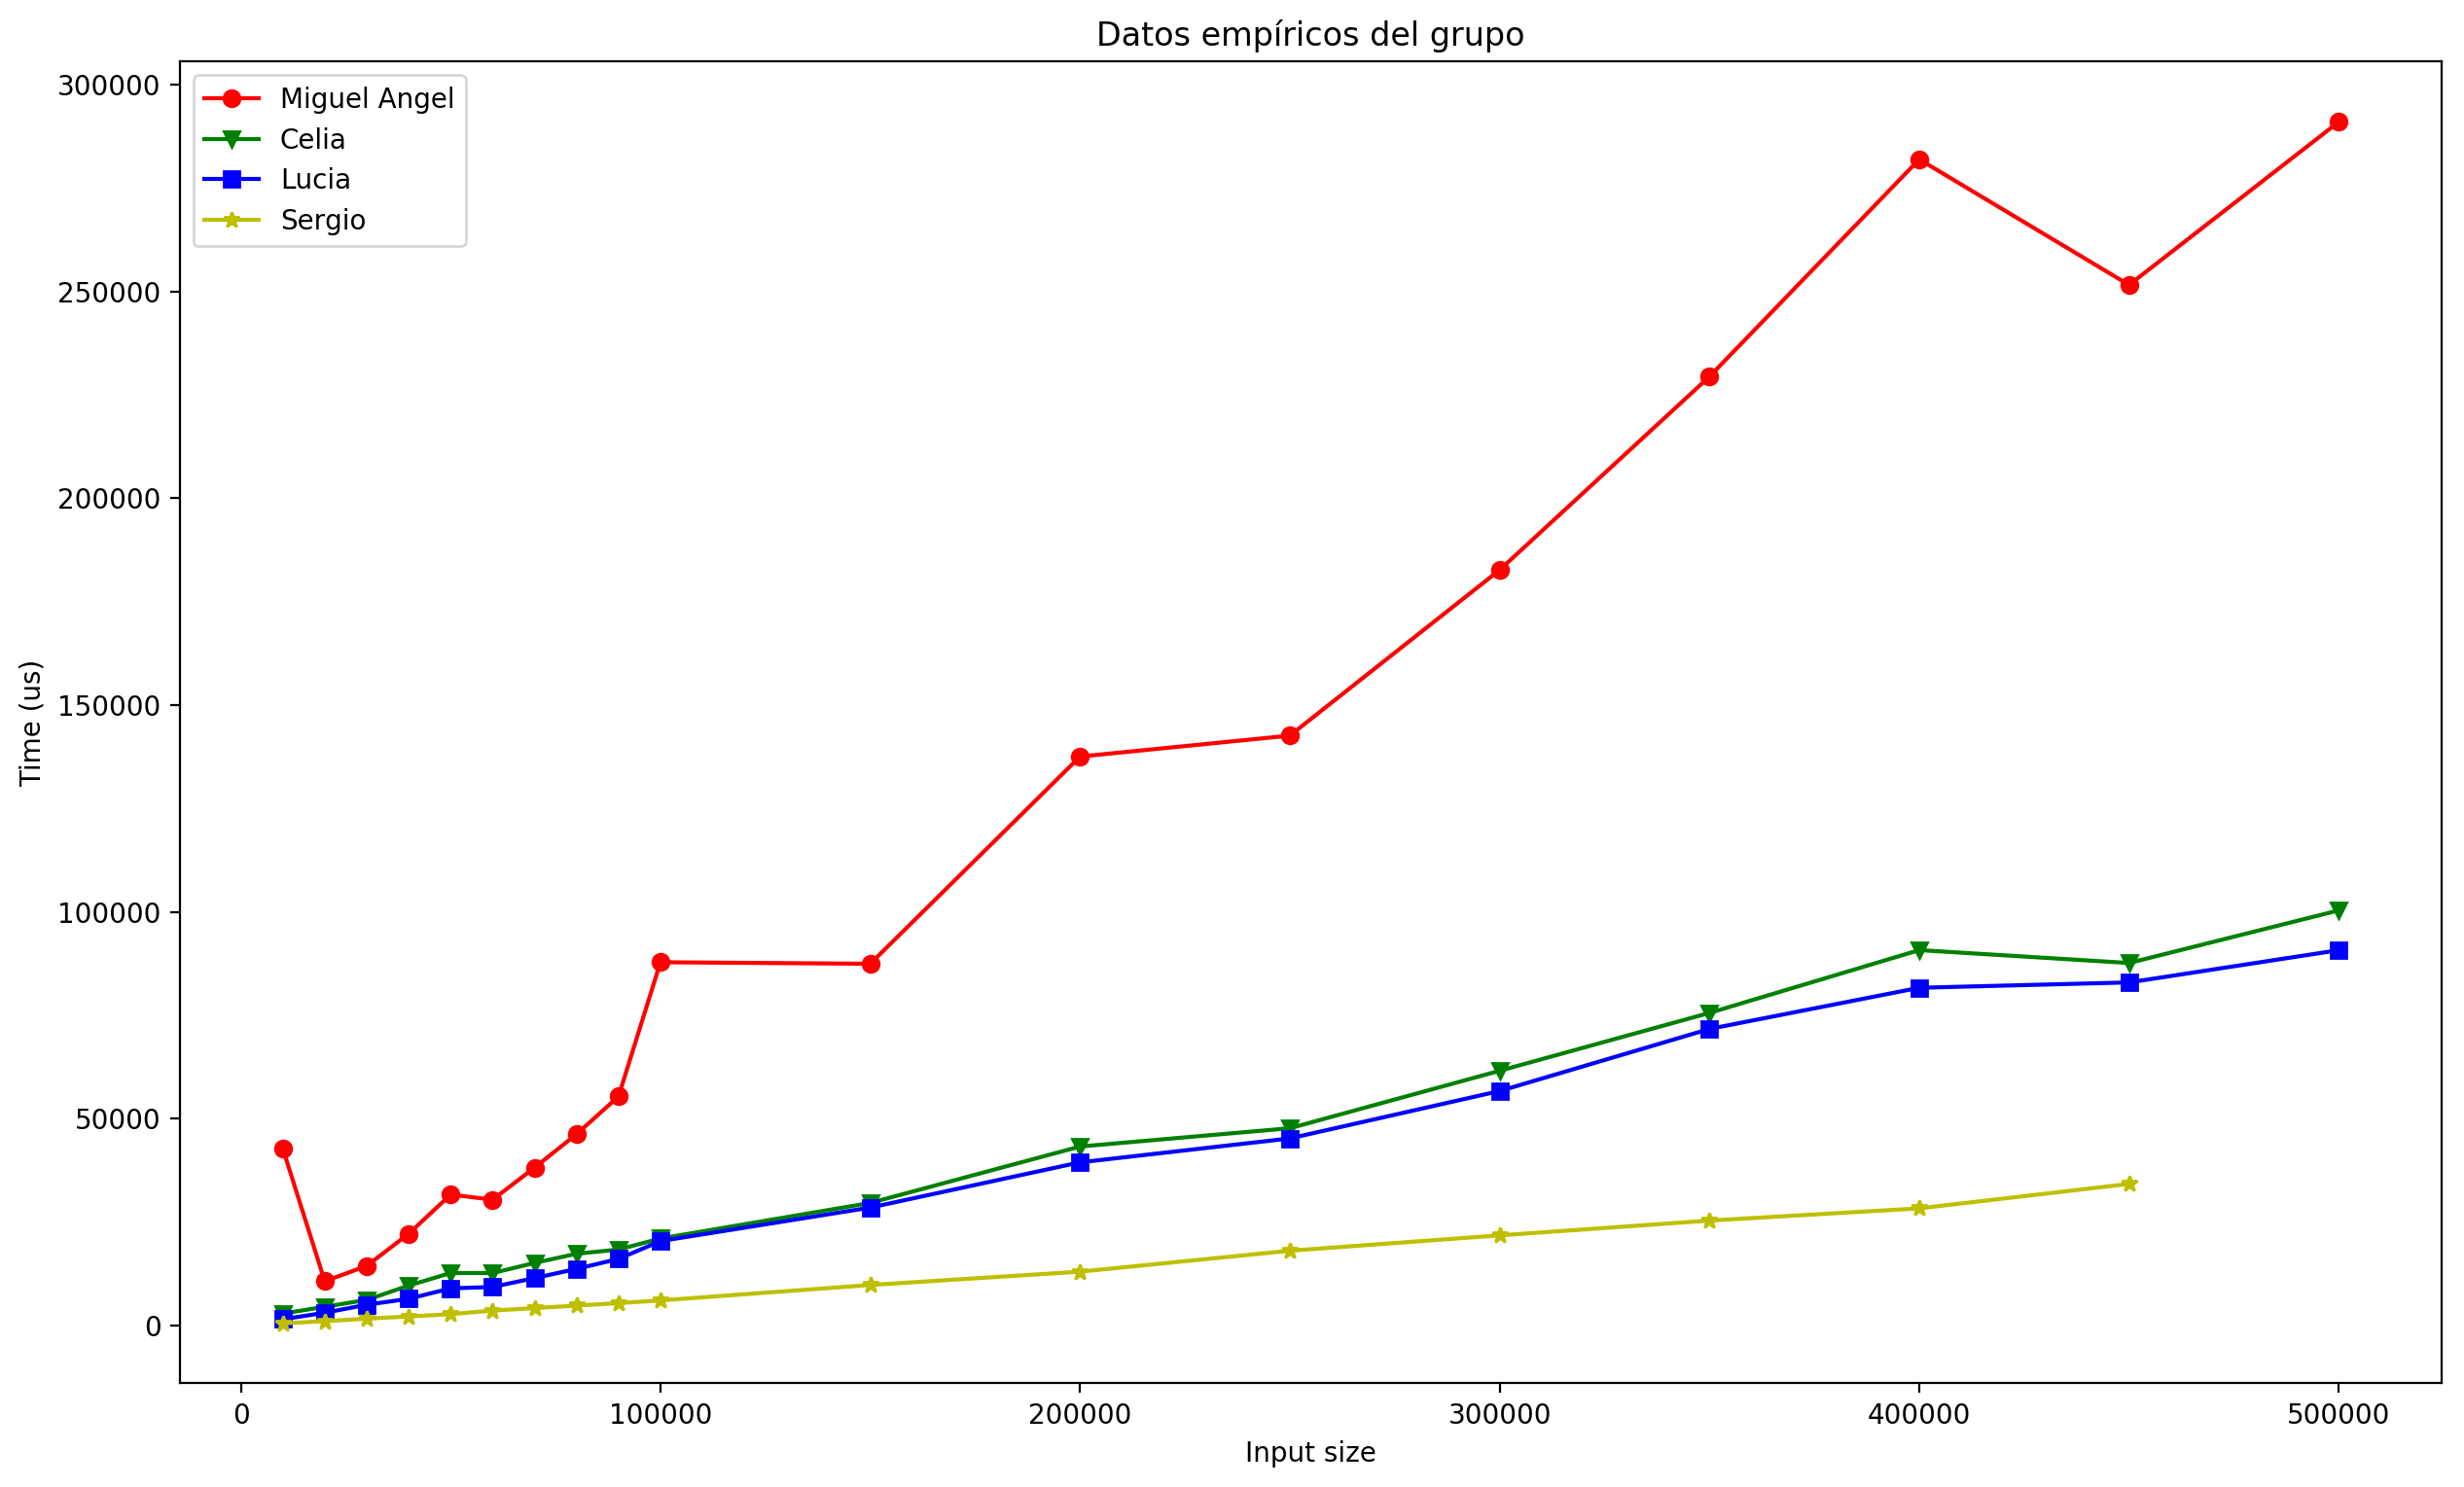
\includegraphics[width=15cm]{./Graficas/merge_todos.png}
	\end{center}
\end{datos}

\subsection{Eficiencia híbrida}

A través de la eficiencia híbrida, comprobaremos que el ajuste teórico realizado es correcto.

Para realizar el análisis de la eficiencia híbrida, tomamos las ejecuciones de uno de los integrantes.
\pagebreak
\begin{datos}
	{\bf\sffamily Gráfico 7.2.} {\sffamily Datos que serán usados para el análisis híbrido}\\
	\vspace{-0.7cm}
	\begin{center}
		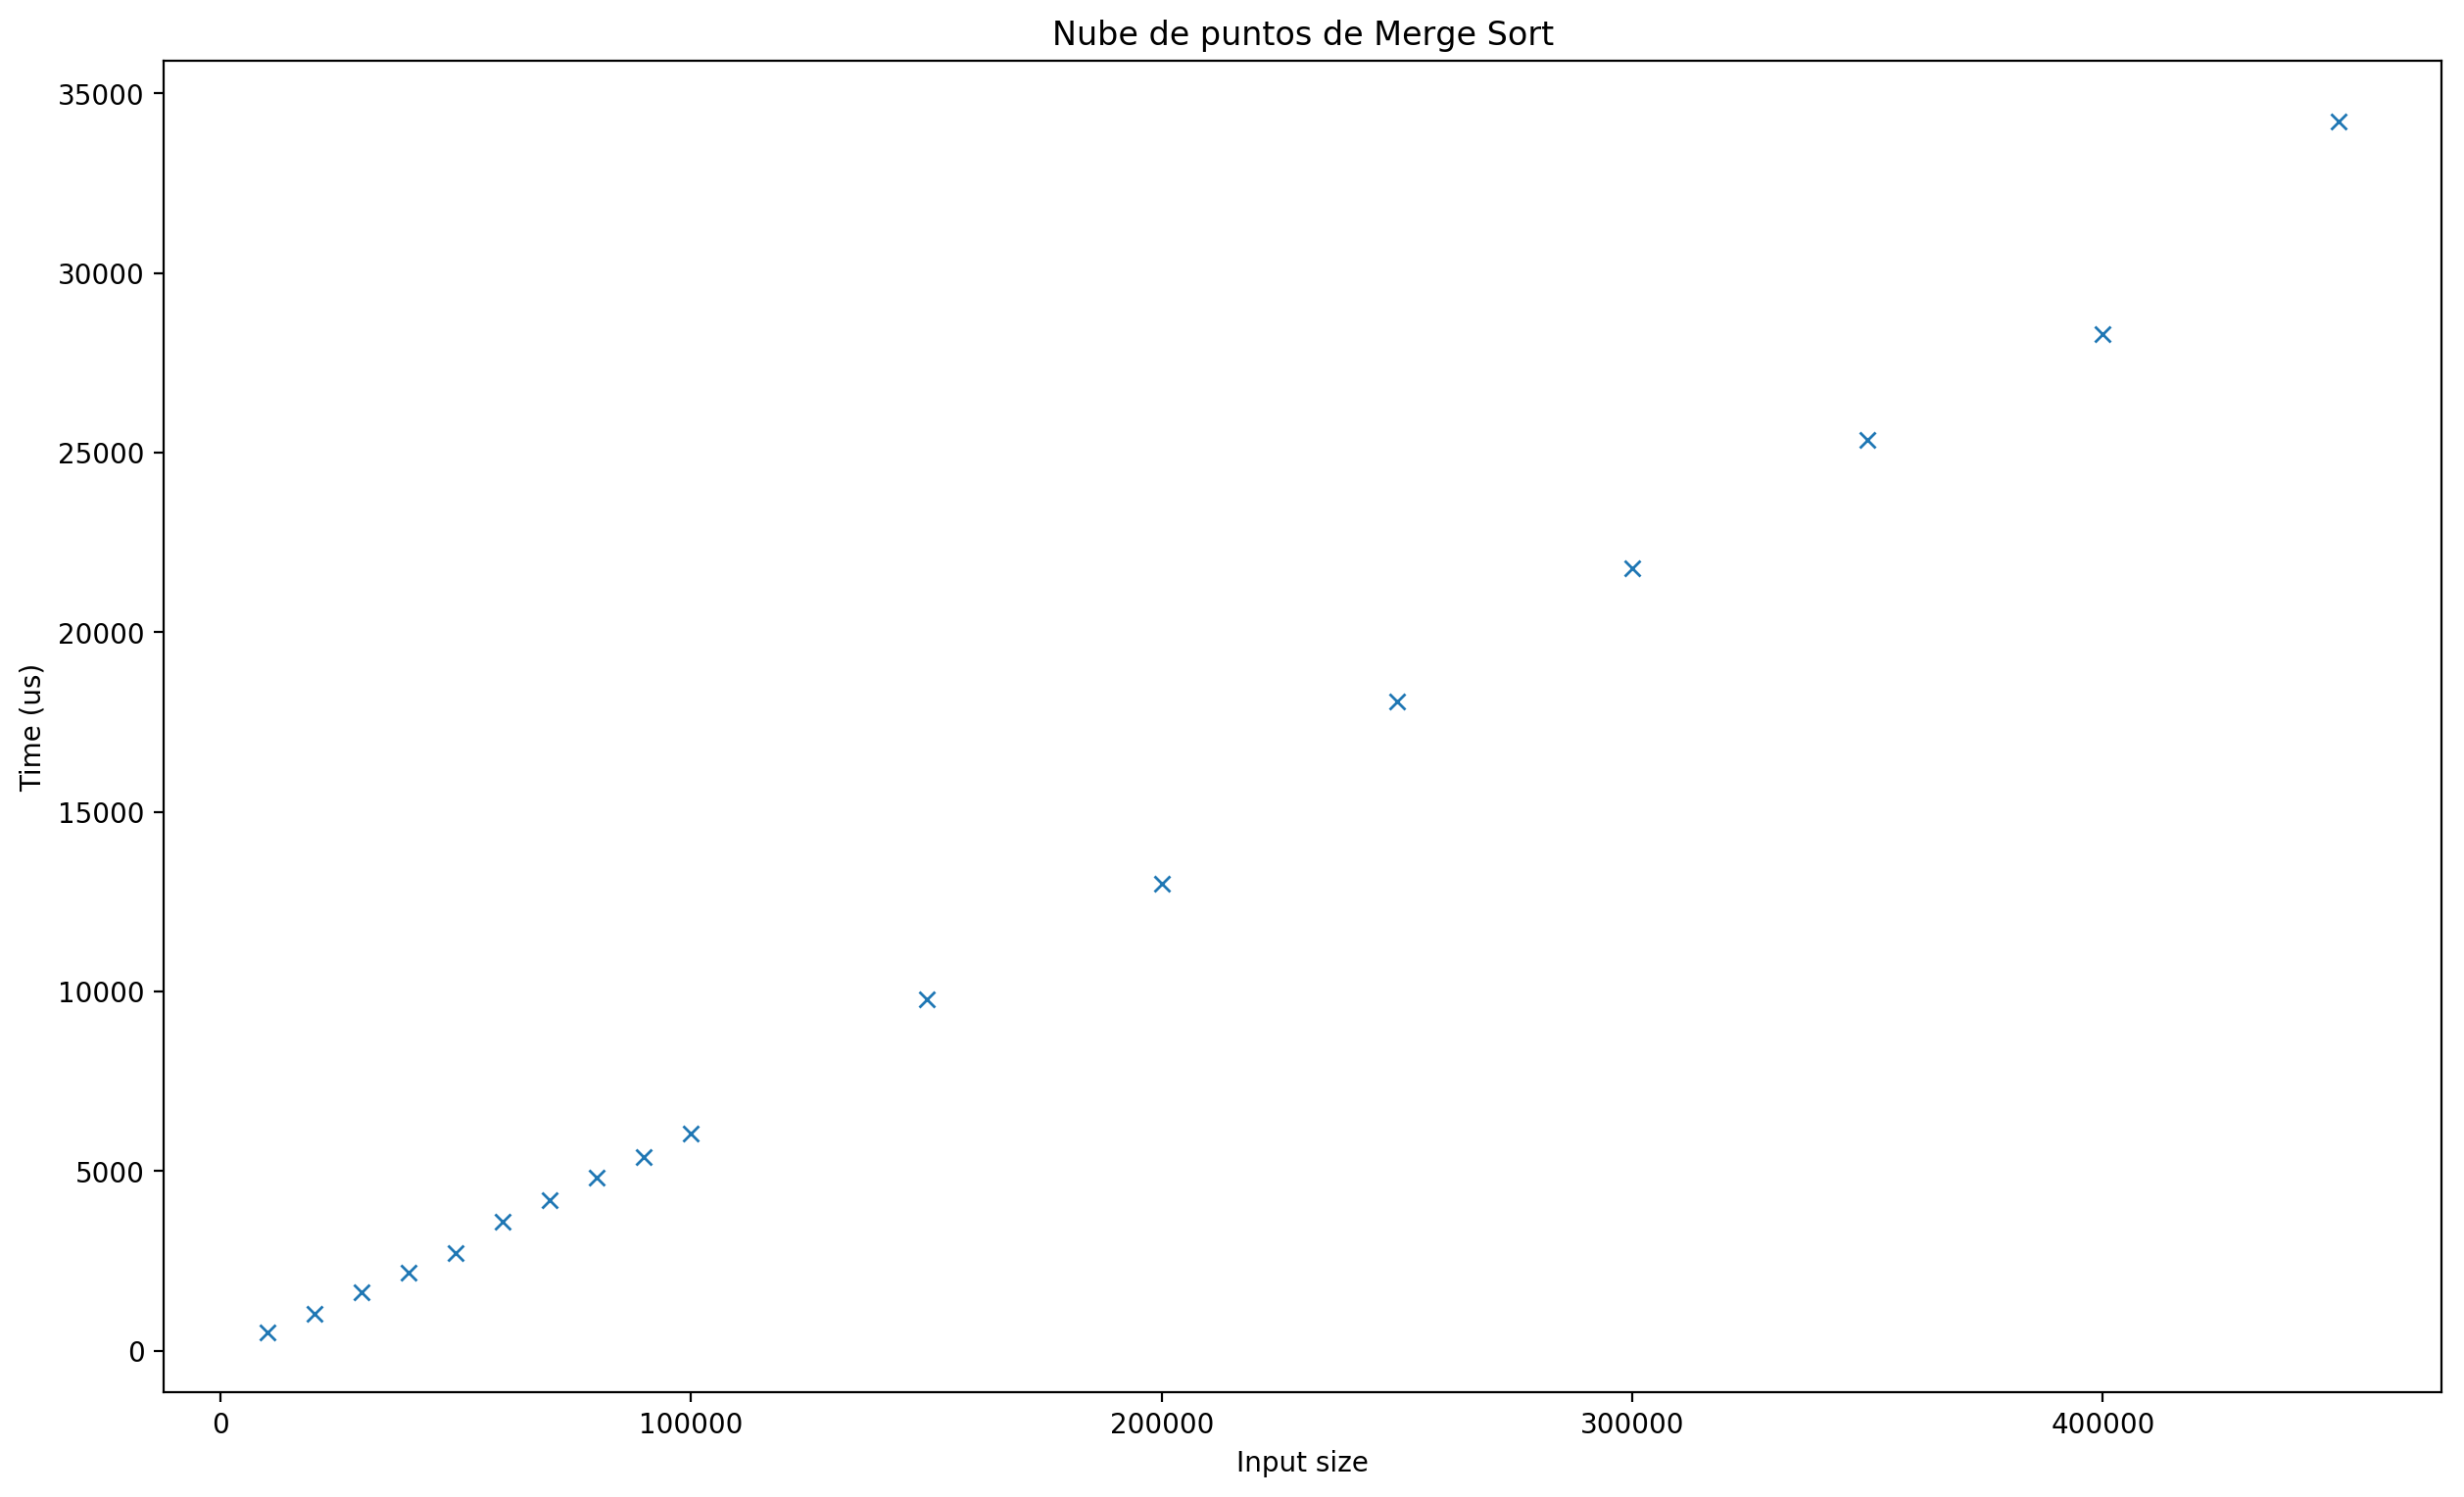
\includegraphics[width=15cm]{./Graficas/merge_nube.png}
	\end{center}	
\end{datos}

\subsubsection{Ajuste de constante oculta}

Tras realizar el ajuste de la constante oculta, el valor obtenido es de $K=1.1670955046281213$.
\pagebreak
\subsubsection{Ajuste por regresión}

\begin{datos}
	{\bf\sffamily Gráfico 7.3.} {\sffamily Ajuste por regresión}\\
	\vspace{-0.7cm}
	\begin{center}
		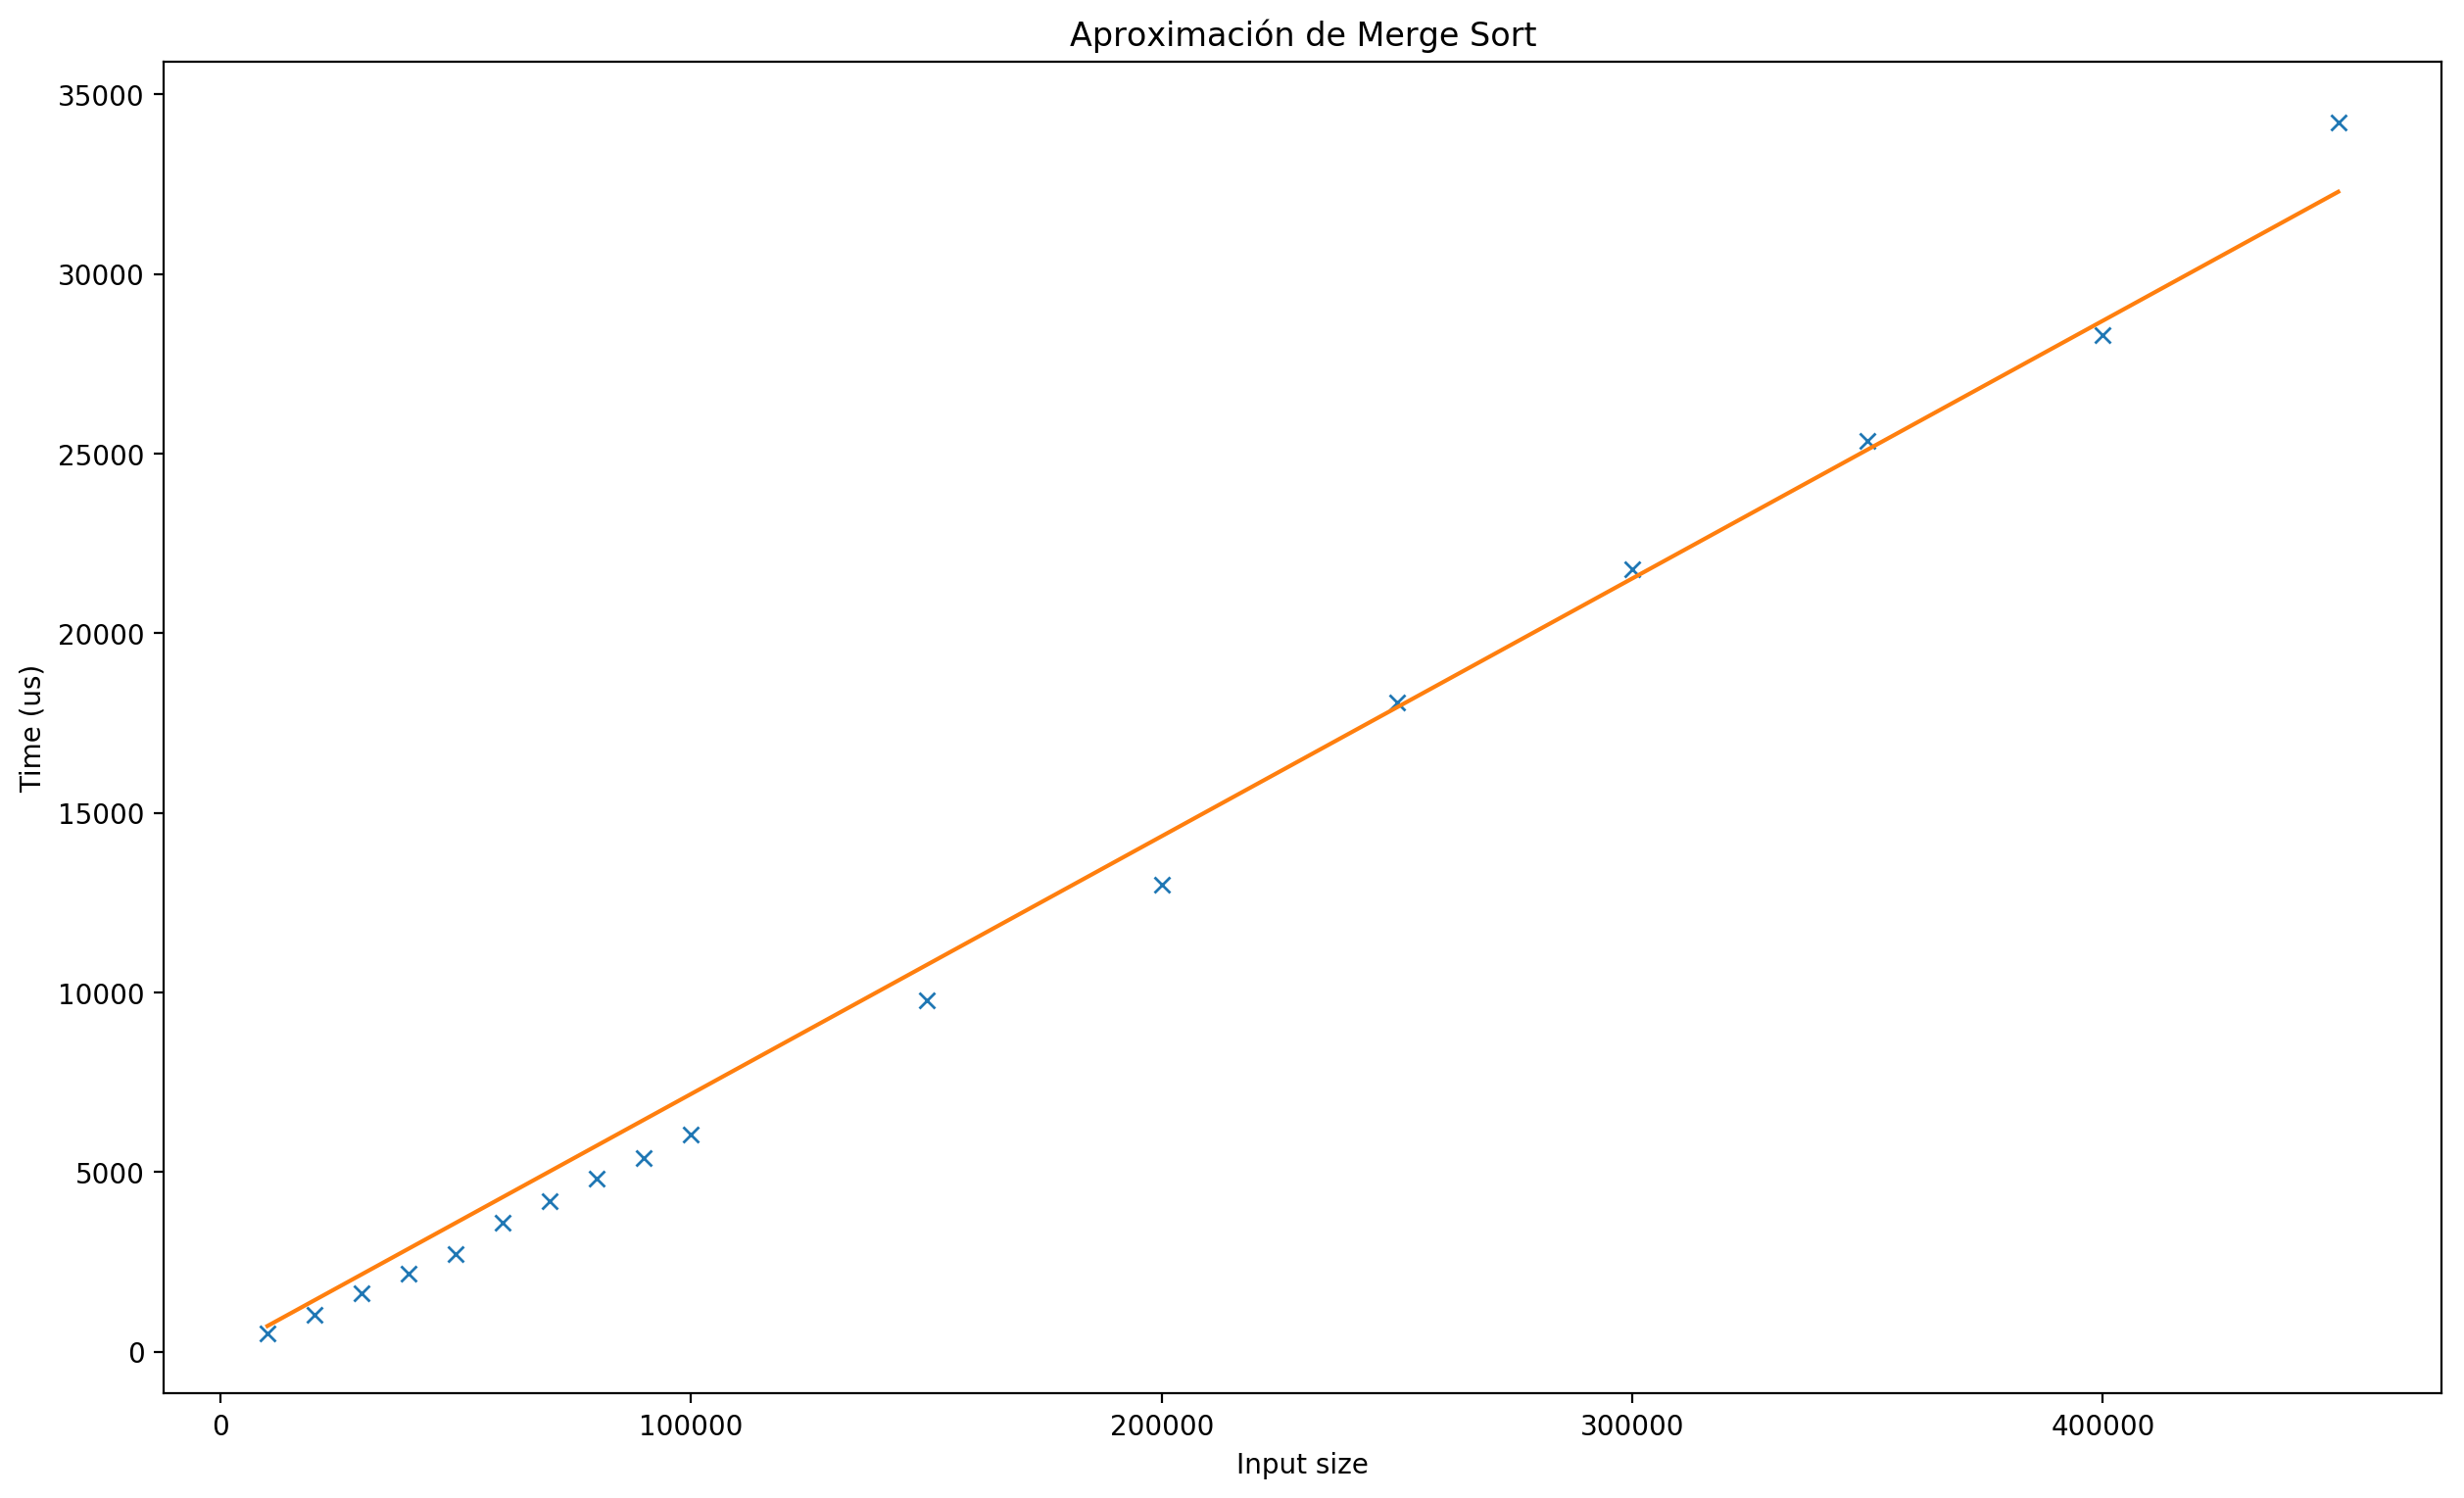
\includegraphics[width=15cm]{./Graficas/merge_ajuste.png}
	\end{center}	
\end{datos}

Realizamos con \emph{Jupyter} el ajuste de regresión para obtener la siguiente función:
$$T(n)=0.07175341\cdot n\log n$$

Que es la que mejor aproxima a nuestros datos. Nótese que es quien tiene el mejor error posible de entre el resto de funciones aproximables (el que tiene mayor error tiene el 100\%, y de ahí los porcentajes restantes son los errores relativos a éste):

\begin{itemize}
	\item Error para recta ($kn$): 0.3473246336299704\%
	\item Error para cuadrática ($kn^2$): 14.334551135315282\%
	\item Error para cúbica ($kn^3$): 37.228355082448616\%
	\item Error para logarítmica ($k\log n$): 100.0\%
	\item \textbf{Error para $\boldsymbol{n}$-logarítmica ($\boldsymbol{kn\log n}$): 0.246638483904476\%}
\end{itemize}
\pagebreak
\section{Algoritmo de las torres de Hanoi}

\begin{lstlisting}[language=C]
void hanoi(int M, int i, int j) {
	if ( M > 0 ) {
		hanoi(M-1, i, 6-i-j);
		hanoi(M-1, 6-i-j, j);
	}
}
\end{lstlisting}

\subsection{Eficiencia teórica}

Estamos ante un algoritmo recursivo, así que buscaremos la relación de recurrencia. Si nos situamos en la iteración $n$-ésima, el algoritmo efectuará una comprobación en el \texttt{if} de eficiencia $O(1)$, y volverá a llamarse a sí misma dos veces. Por tanto, la ecuación de recurrencia que caracteriza a este algoritmo es:
$$ T_n=2T_{n-1}+1$$
Despejando y operando, resolvemos esta recurrencia:
$$ (x-2)(x-1)=0 $$
$$ t_n=c_1\cdot 2^n + c_2 \cdot 1^n = c_1 \cdot 2^n + c_2$$

En definitiva, nuestro algoritmo tiene una eficiencia $\boldsymbol{O(2^n)}$.


\subsection{Eficiencia empírica}

Tras ejecutar el algoritmo con \texttt{M} desde 2 hasta 30, los resultados de ejecución para cada uno de los miembros del grupo fueron los siguientes:
\pagebreak
\begin{datos}\hspace{-0.2cm}
	{\bf\sffamily Gráfico 8.1.} {\sffamily Datos de todas las ejecuciones}\\
	\vspace{-0.7cm}
	\begin{center}
		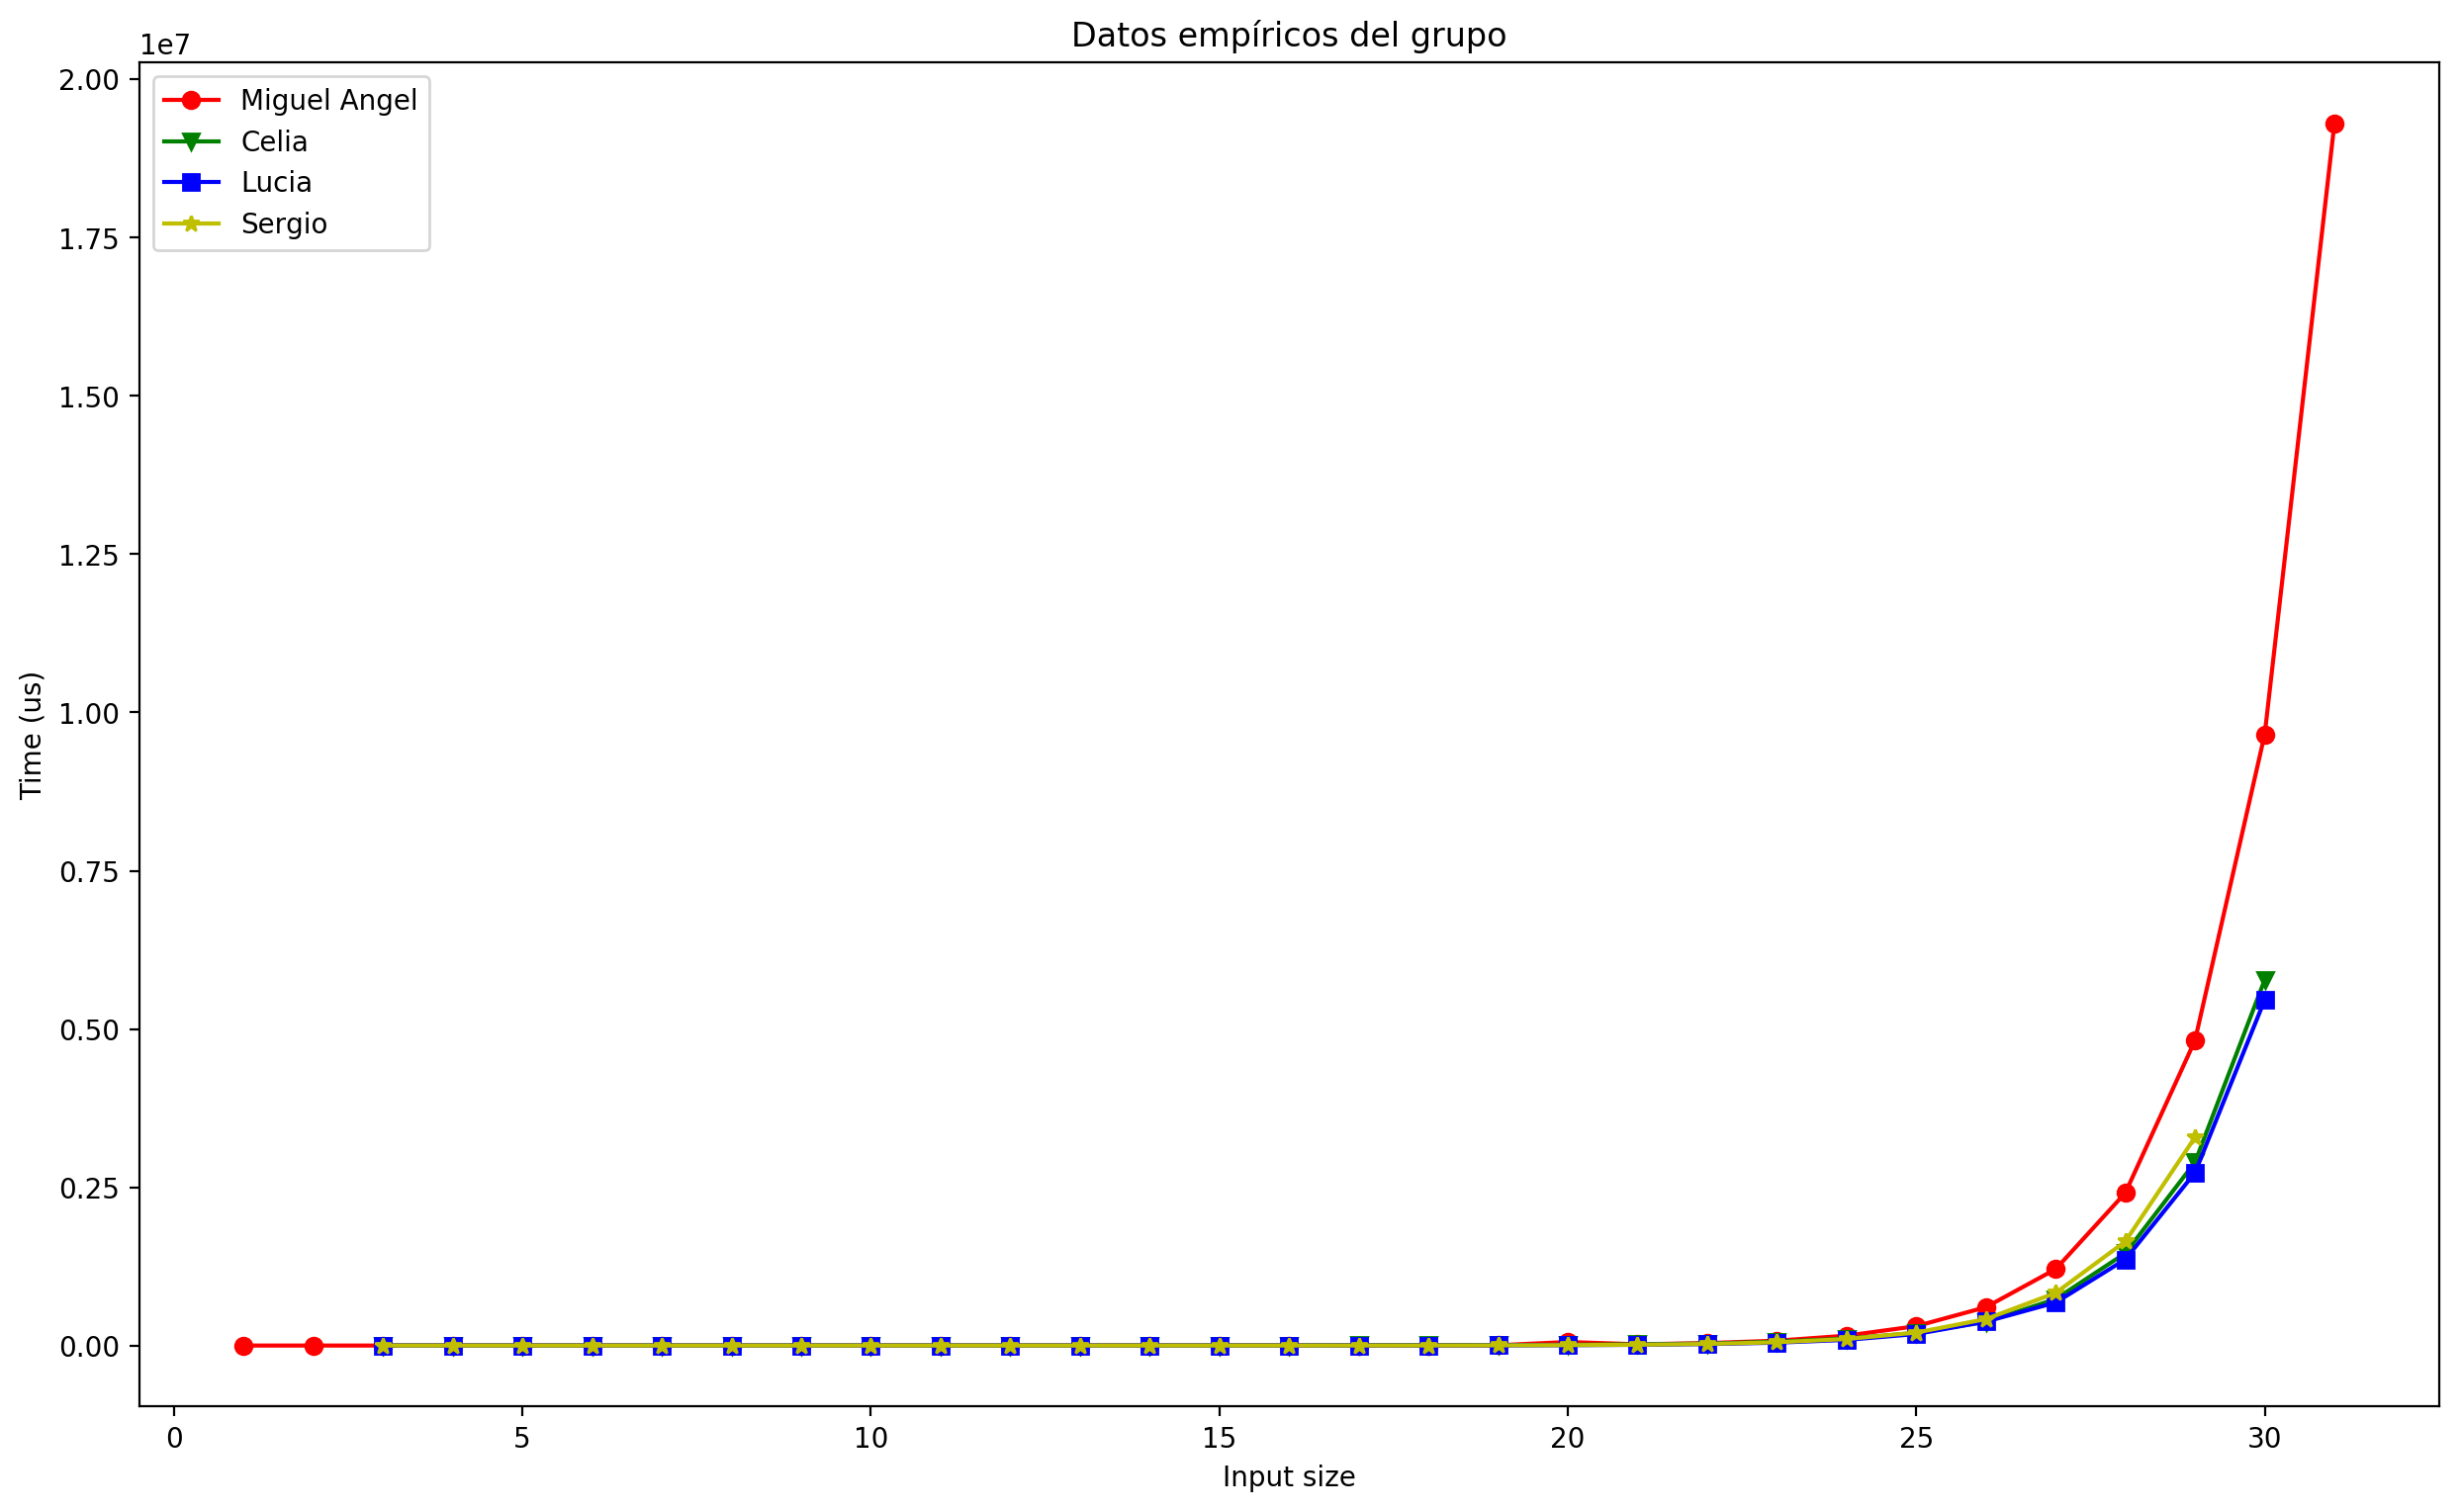
\includegraphics[width=15cm]{./Graficas/hanoi_todos.png}
	\end{center}
\end{datos}

\subsection{Eficiencia híbrida}

A través de la eficiencia híbrida, comprobaremos que el ajuste teórico realizado es correcto.

Para realizar el análisis de la eficiencia híbrida, tomamos las ejecuciones de uno de los integrantes.
\pagebreak
\begin{datos}
	{\bf\sffamily Gráfico 8.2.} {\sffamily Datos que serán usados para el análisis híbrido}\\
	\vspace{-0.7cm}
	\begin{center}
		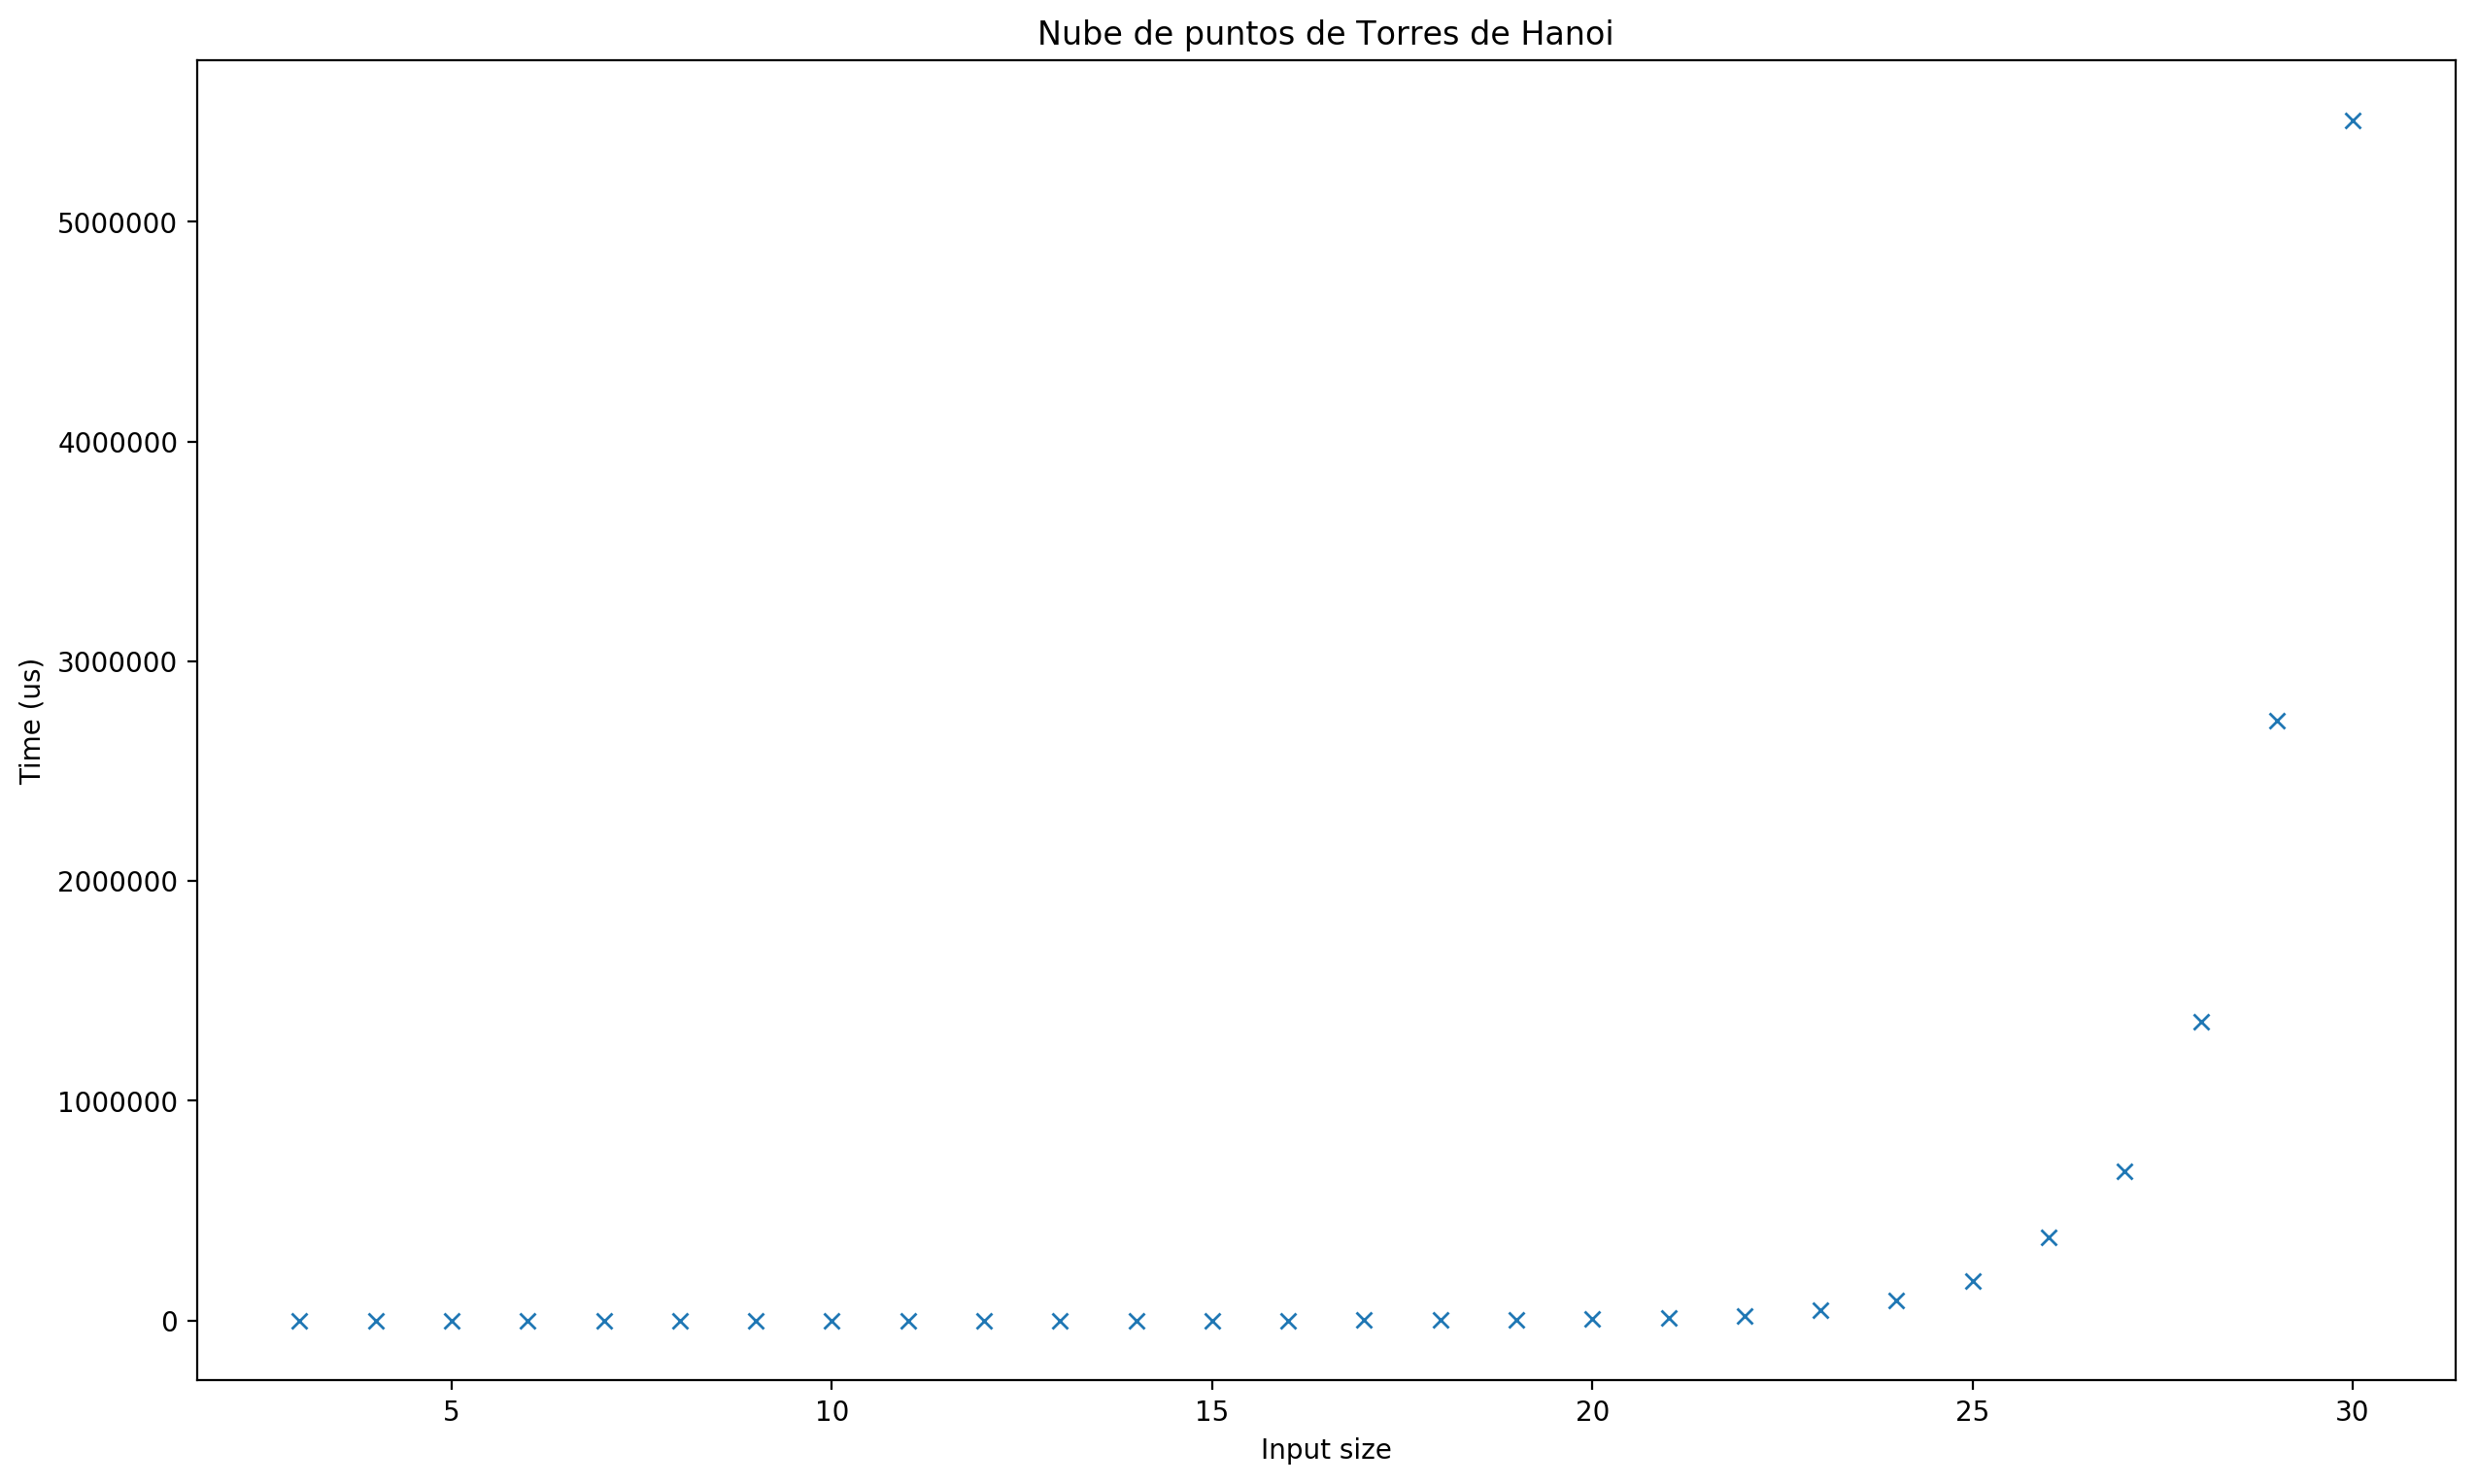
\includegraphics[width=15cm]{./Graficas/hanoi_nube.png}
	\end{center}	
\end{datos}

\subsubsection{Ajuste de constante oculta}

Tras realizar el ajuste de la constante oculta, el valor obtenido es de $K=0.7263436302553232$.

\subsubsection{Ajuste por regresión}

\begin{datos}
	{\bf\sffamily Gráfico 8.3.} {\sffamily Ajuste por regresión}\\
	\vspace{-0.7cm}
	\begin{center}
		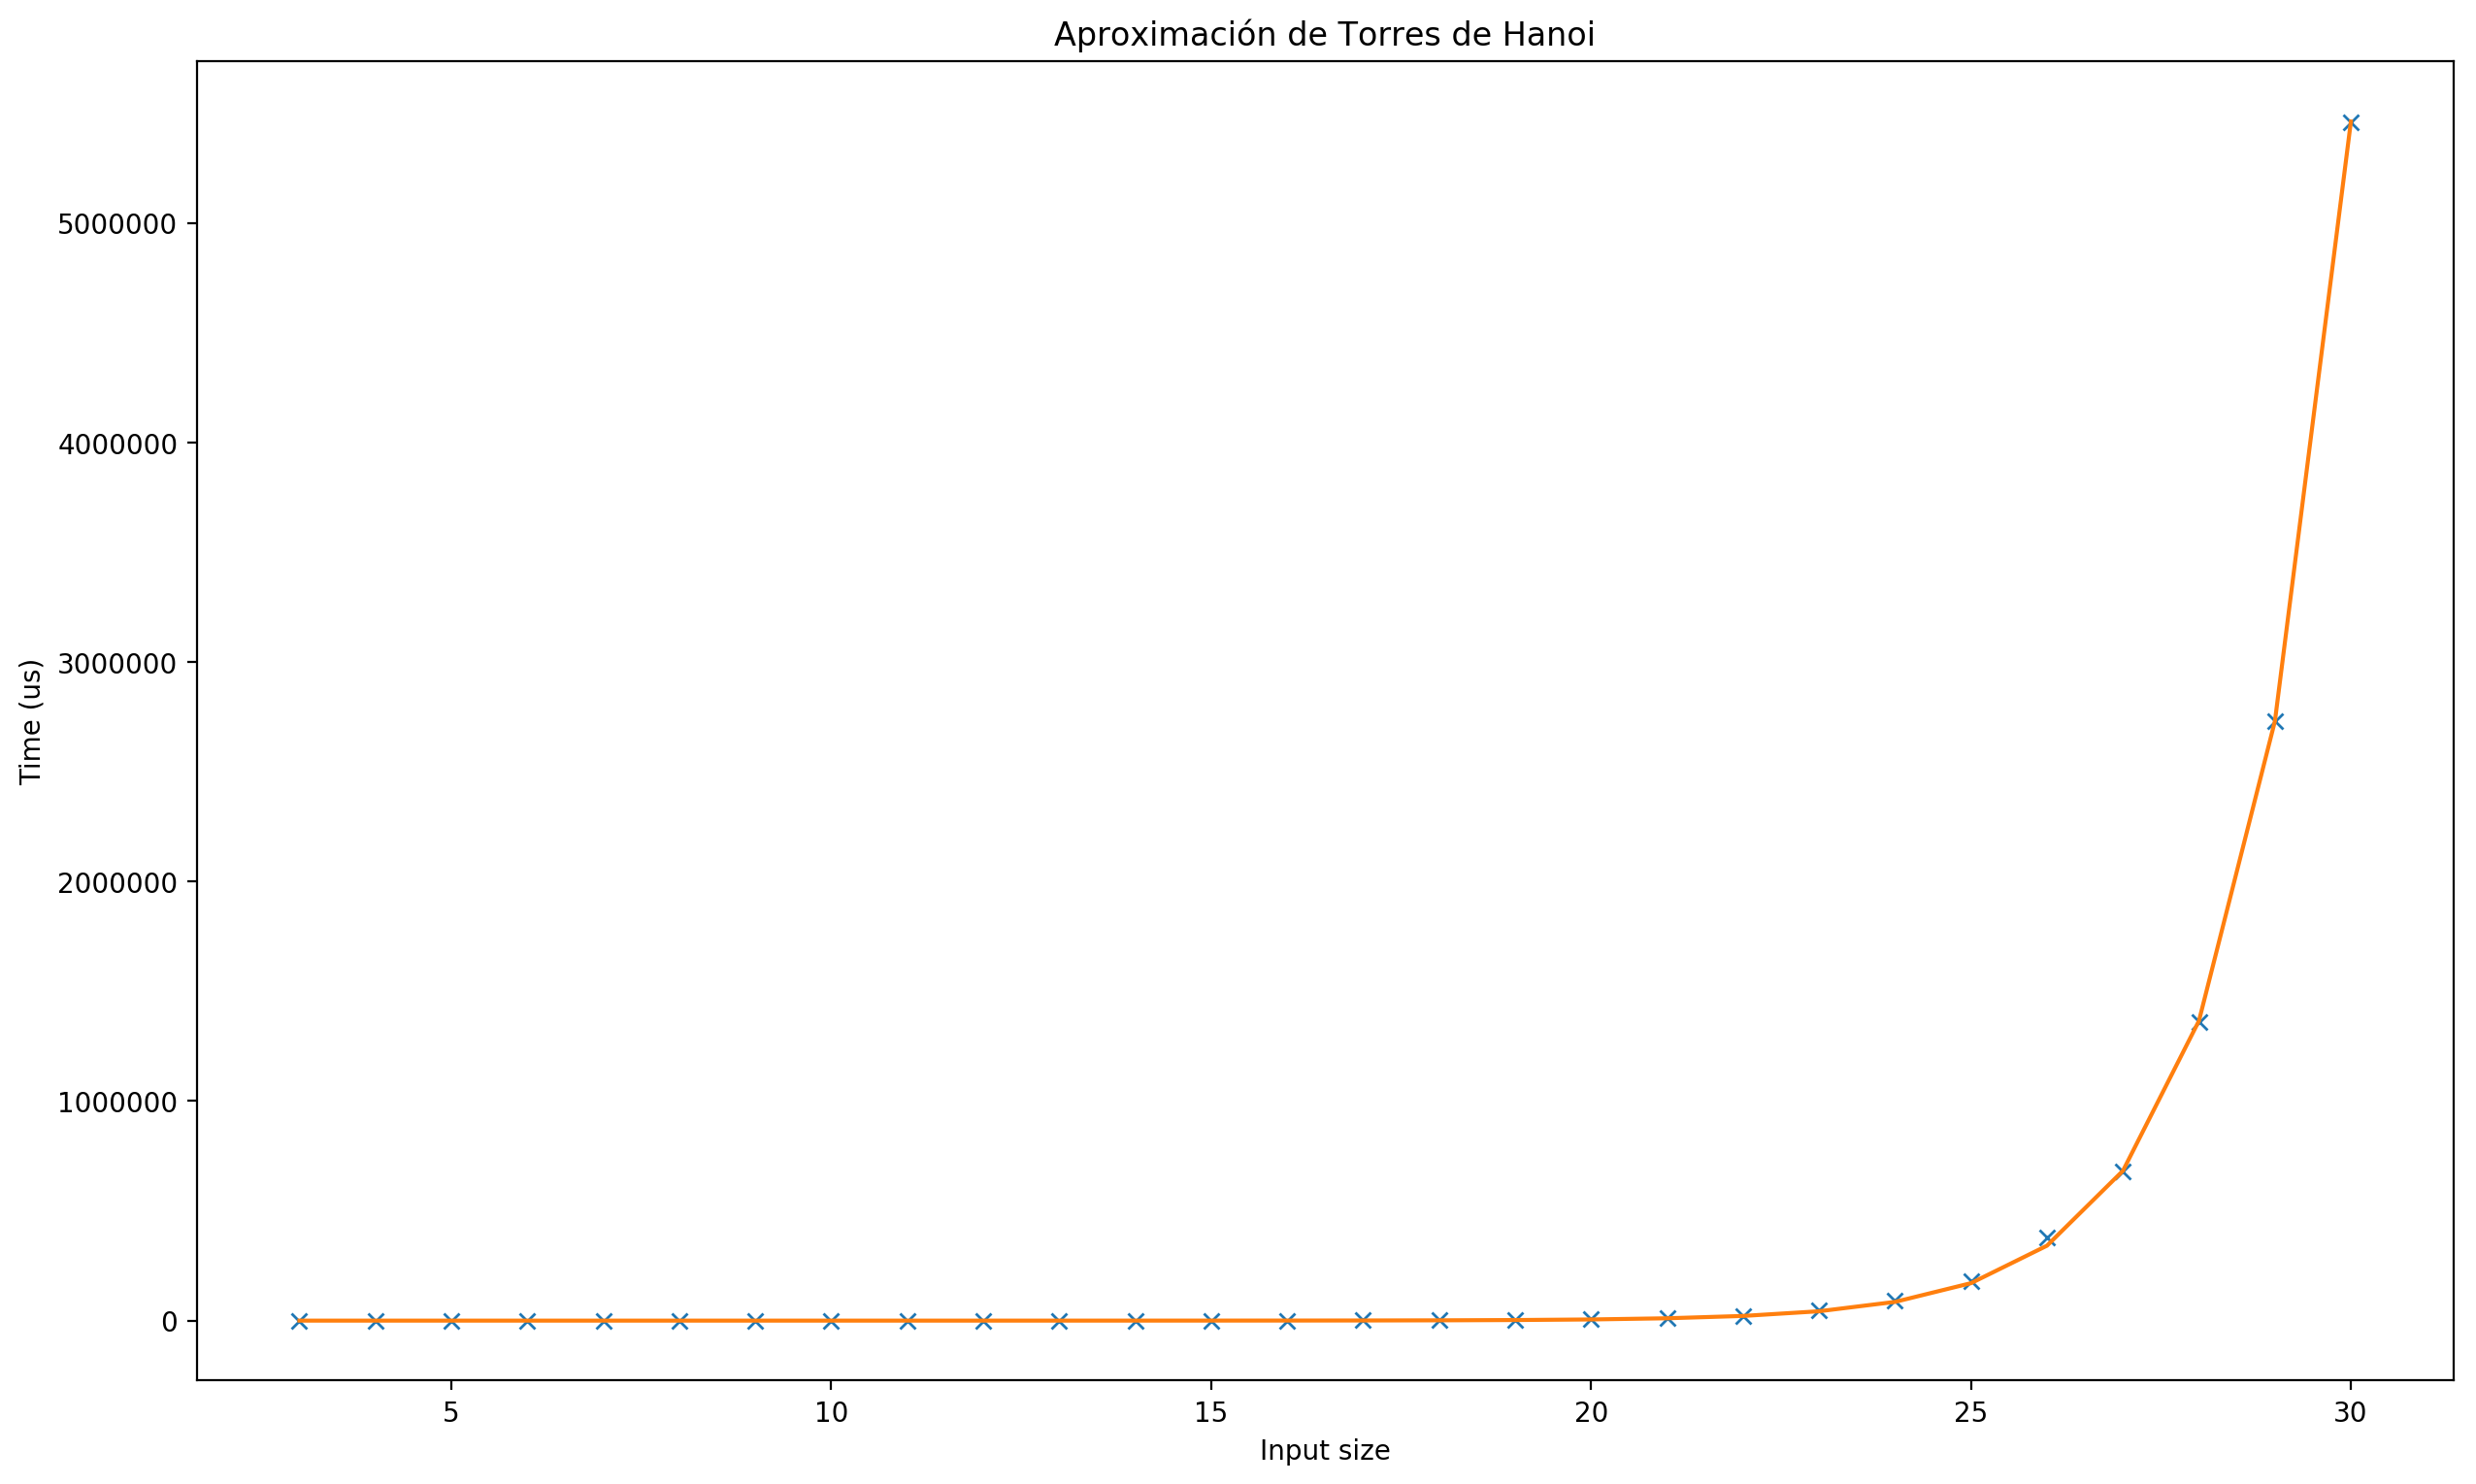
\includegraphics[width=15cm]{./Graficas/hanoi_ajuste.png}
	\end{center}	
\end{datos}

Realizamos con \emph{Jupyter} el ajuste de regresión para obtener la siguiente función:
$$T(n)=0.00508635\cdot 2^n$$

Que es la que mejor aproxima a nuestros datos. Nótese que es quien tiene el mejor error posible de entre el resto de funciones aproximables (el que tiene mayor error tiene el 100\%, y de ahí los porcentajes restantes son los errores relativos a éste):

\begin{itemize}
	\item Error para recta ($kn$): 76.01343903600339\%
	\item Error para cuadrática ($kn^2$): 71.13401593179258\%
	\item Error para cúbica ($kn^3$): 57.61256154034523\%
	\item Error para exponencial ($ke^n$): 3.1920070654956563\%
	\item \textbf{Error para potencial ($k2^n$): 0.004591299781178793\%}
	\item Error para logarítmica ($k\log n$): 100.0\%
\end{itemize}


\pagebreak
\part{Conclusiones}

Tras realizar los análisis teóricos de los diversos algoritmos, hemos visto que con los datos obtenidos empíricamente y utilizando una curva de regresión podemos ajustar adecuadamente a la función que deberíamos obtener. Con todo esto, deducimos que nuestro análisis teórico ha sido correcto. 

También hemos podido comprobar que los datos obtenidos en la práctica dependen de la arquitectura del ordenador de cada componente del grupo, aún así las funciones son las mismas, siendo esto de mayor relevancia en el análisis de algoritmos.

\section*{Comparación entre algoritmos de búsqueda}
Tras haber ejecutado los códigos y haber analizado los algoritmos teóricamente hemos comprobado que \emph{Heap Sort} y \emph{Merge Sort} son notablemente mejores que \emph{Bubble Sort}. Esto se debe a que el orden de eficiencia de los primeros es $n\log n$, al contrario que \emph{Bubble Sort}, que es $n^2$.

\begin{datos}
	{\bf\sffamily Gráfico III.1.} {\sffamily Comparación entre algoritmos de búsqueda}\\
	\vspace{-0.7cm}
	\begin{center}
		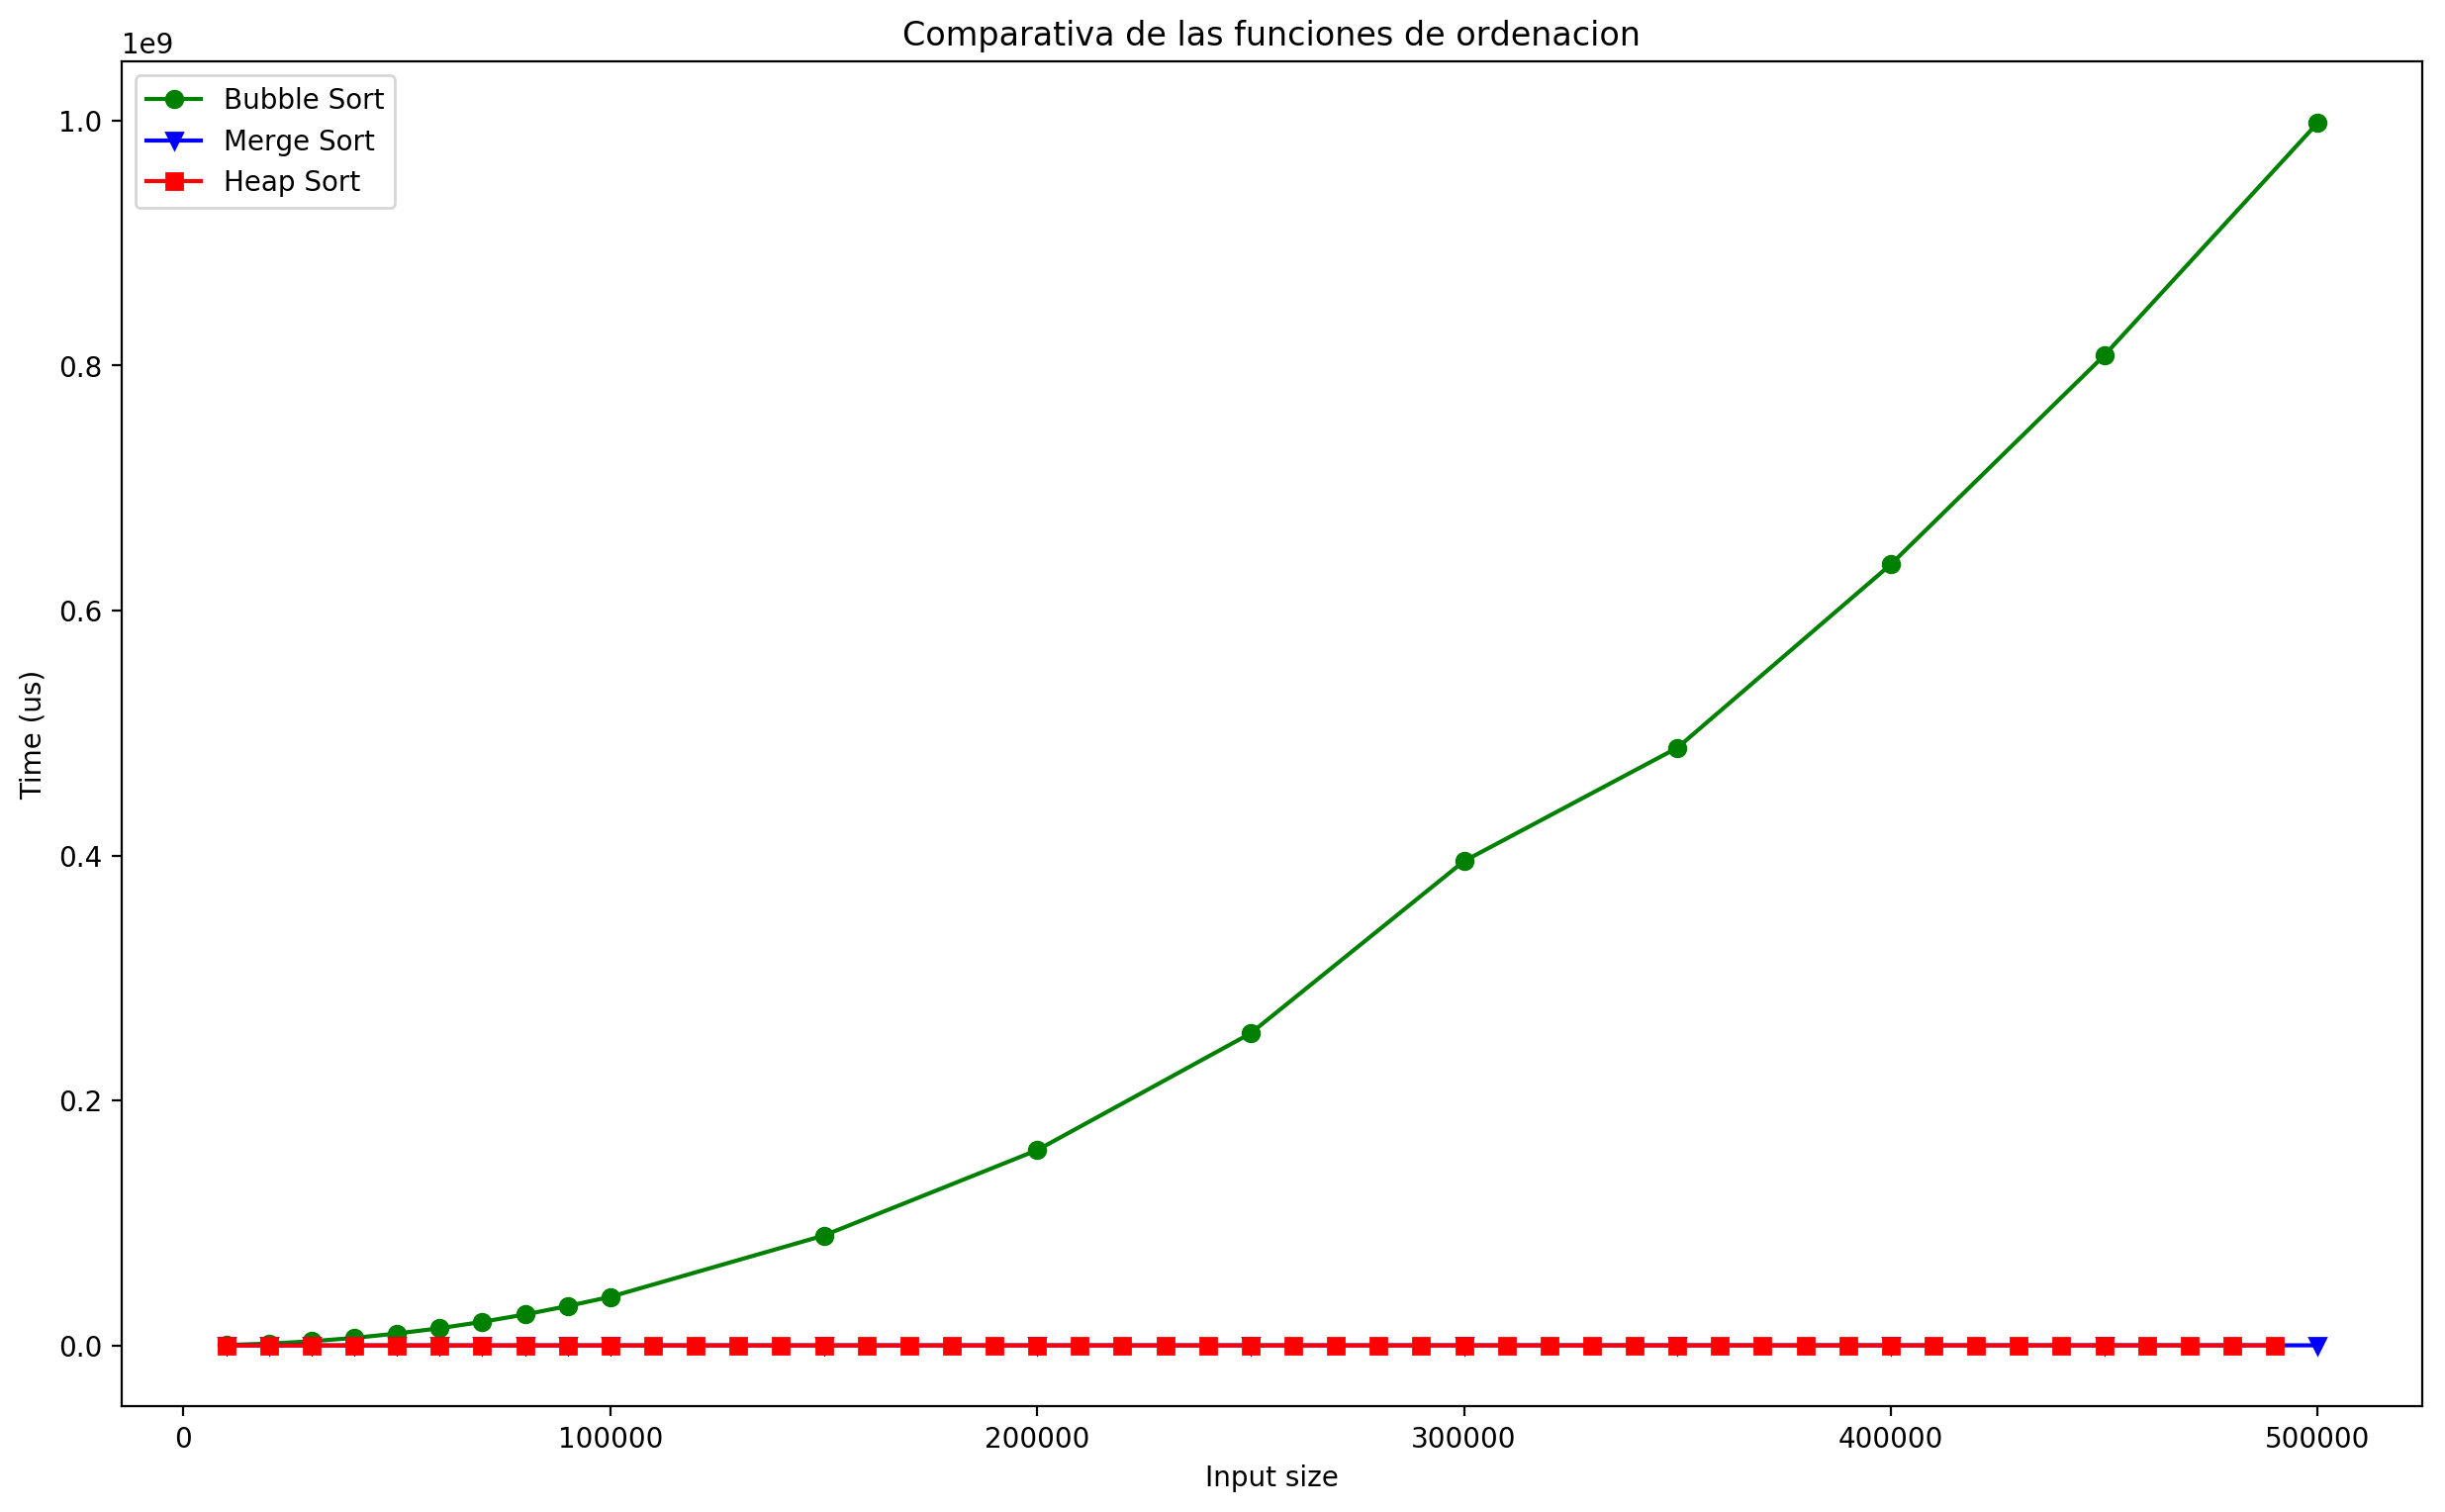
\includegraphics[width=15cm]{./Graficas/comparativa_todas.png}
	\end{center}	
\end{datos}

Ya que la diferencia es aplastante, nos centraremos en los algoritmos \emph{Merge Sort} y \emph{Heap Sort}.
\pagebreak
\begin{datos}
	{\bf\sffamily Gráfico III.2.} {\sffamily Comparación entre algoritmos de búsqueda: \emph{Merge Sort} y \emph{Heap Sort}}\\
	\vspace{-0.7cm}
	\begin{center}
		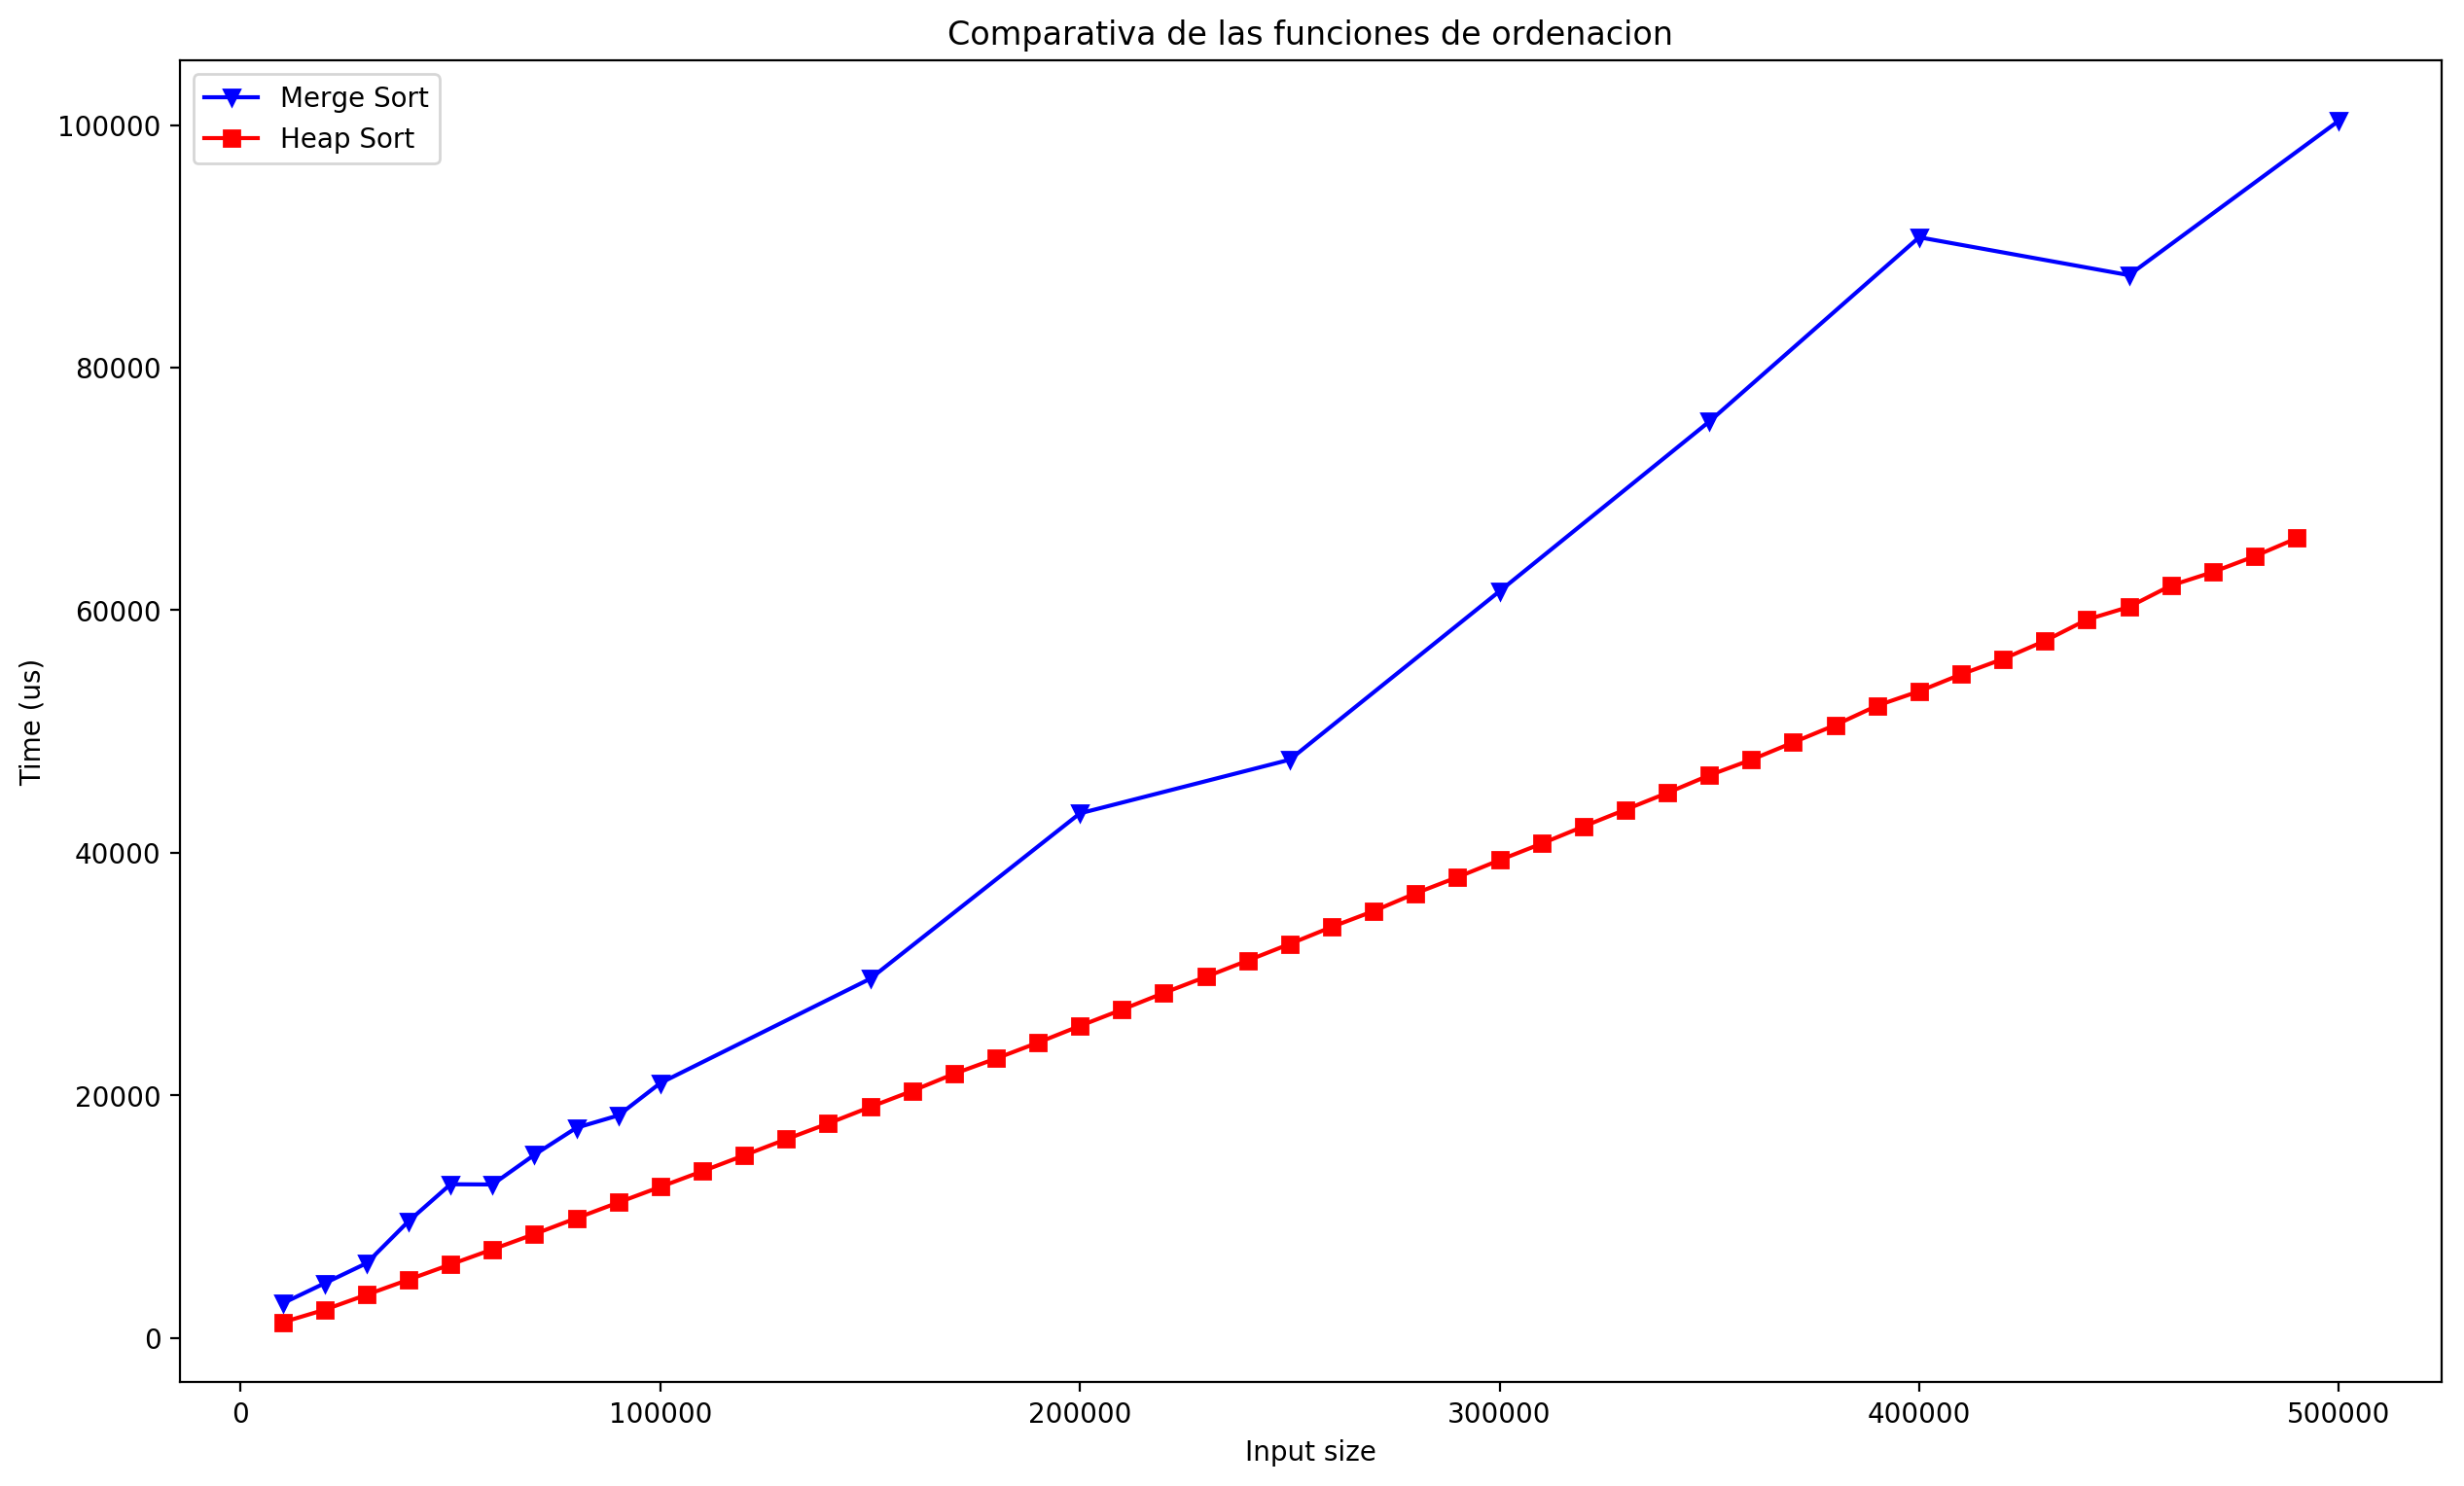
\includegraphics[width=15cm]{./Graficas/comparativa_merge_heap.png}
	\end{center}
\end{datos}
Entre estos dos algoritmos con orden de eficiencia mejor, podemos ver que, tras haber realizado un estudio experimental de ambos, el mejor de ellos es \emph{Heap Sort}.

\end{document}
